\chapter{\texorpdfstring{Search for MSSM \AHtotautau}{Search for MSSM A/H -->tautau}}
\label{chap:mssm}
In this chapter the search for neutral Higgs bosons \PHiggs or \PHiggsps
decaying to a pair of \Pgt leptons will be discussed. The results presented
here correspond to those from an analysis peformed on a dataset collected
during the first half of the 2016 p--p running period of the \ac{LHC}. This dataset
corresponds to an integrated luminosity of 12.9 fb$^{-1}$, and the analysis is
detailed in Ref. \cite{CMS-PAS-HIG-16-037}. The \etau, \mutau, \tautau and \emu final
states of the di-\Pgt pair were studied. The results of this search are 
model--independent upper limits on $\sigma \times$ BR of \PHiggs or \PHiggsps 
production in the gluon fusion (gg$\phi$) and b-associated (bb$\phi$) production 
modes (see chapter \ref{chap:theory}) and decay into $\Pgt\Pgt$. 
In addition to the upper limits on cross--section times branching ratio of these two processes, 
the results are interpreted in MSSM benchmark scenarios.
A very similar analysis, not described in detail here,
was performed on a dataset corresponding to 2.3 fb$^{-1}$ collected at $\sqrt{s}=13$ TeV during the 2015 \ac{LHC} p--p running period.  
More information can be found in reference \cite{CMS-PAS-HIG-16-006}.

For the analysis described in this chapter, as well as the 2015 analysis,
I was responsible for all stages of the analysis. This included optimisation 
of object selection and categorisation,
as well as studies of background methods for the \mutau, \etau and \tautau channels,
evaluation of systematic uncertainties in all four channels, and production of
the statistical results, including model interpretations.

\section{Datasets and \acs{MC} samples}
\label{sec:mssm_datasets}
The dataset used for this analysis corresponds to an integrated 
luminosity of 12.9 fb$^{-1}$ collected at a centre--of--mass
energy of 13 TeV during the first half of
the 2016 p--p running period of the \ac{LHC}. %Section
%\ref{sec:mssm_combination} includes the combination of this
%dataset with a dataset collected during the 2015 p--p running
%period of the \ac{LHC}. This dataset corresponds to an integrated
%luminosity of 2.3 fb$^{-1}$ collected at $\sqrt{s} = 13$ TeV.

Signal and background events were generated using
various \ac{MC} event generators. Signal samples
for the $\Pg\Pg \rightarrow \phi$ and $\Pg\Pg \rightarrow b\bar{b}\phi$
production processes of $\PHiggs/\PHiggsps$ were generated using \texttt{PYTHIA 8.1} \cite{pythia81}.
These samples were produced for a range of masses between 90 GeV and 3.2 TeV.
This range is slightly wider than the range in which MSSM Higgs sector
benchmark computations are available, 90 GeV -- 2 TeV, and 
improves on the mass range of 90 GeV to 1 TeV that was studied during Run 1 in the context of BSM Higgs searches.
SM Higgs signal samples are used for the interpretation of the analysis results in 
MSSM benchmark scenarios. These samples are generated using \texttt{Powheg} \cite{powheg1,powheg2,powheg3}.

Single-top and \ttbar background samples are generated using \texttt{Powheg},
with \texttt{MadGraph5\_aMC@NLO} \cite{amcnlo} used for the generation of di--boson background
samples. %and part of the W+$\gamma$ background, which is included in the \emu channel only.
\Wjets and \Zll backgrounds are generated with the \texttt{MadGraph 5} \cite{madgraph}
matrix element generator. Samples containing both a mixture
of jet multiplicities (`inclusive' samples) and samples with 1,2,3 or 4 jets (`exclusive' samples)
are generated. These exclusive samples increase the available number of
background events with higher jet multiplicities. %note LO samples used because to get same number of effective
%events would need to generate more NLO samples
The `inclusive' and `exclusive' samples are reweighted
before they are combined so as to preserve the correct
fractions of events with each jet multiplicity. The $\PW+\Pphoton$ background samples,
only included in the \emu channel, is generated in part with \texttt{MadGraph 5} and in
part with \texttt{MadGraph5\_aMC@NLO}.

Parton showering and hadronisation are modelled using \texttt{PYTHIA 8.1} for all 
samples, and  minimum--bias events generated with \texttt{PYTHIA 8.1} are
added to all \ac{MC} samples to model additional interactions. A reweighting
is then applied to the \ac{MC} samples to make the pile--up distribution match
the pile--up distribution observed in data.

\section{Event selection and categorisation}
\label{sec:mssm_eventsel}
In this section an overview of the event selection,
and how it was optimised, is given. More detailed information
on how the objects used are reconstructed, 
and a more in--depth description of the identification criteria, 
is given in chapter \ref{chap:objects}.

The basis of the event selection is to identify \mutau, \etau,
\tautau and \emu pairs. Events are selected first by using a trigger,
followed by additional selection criteria. For the \etau
and \mutau channels we only trigger on the electron or muon. 
While the lepton + hadronic tau cross triggers that are also available
allow for a 3 (6) GeV lower \pT~threshold on the
muon (electron), the benefit of using such a trigger is small as 
most of the signals at high-mass, the region of interest in this
analysis, have higher \pT~electrons and muons. This is illustrated
in figure \ref{fig:mt_muonpt}a, which shows the \pT~of muons in the
\mutau channel, with the signal normalised to 4000 times its cross--section
times branching ratio at \mA=1 TeV and \tanb=50 in the $m_{h}^{\text{mod}+}$ scenario overlaid.
In the \emu channel two dedicated electron-muon cross triggers
are used. These have significantly lower online \pT~cuts 
on the two leptons than the single lepton triggers. For the 
\tautau channel a di-tau cross-trigger is used.

Because the triggers involving electrons or muons reach 
their maximum efficiency as a function of \pT~quickly, the offline \pT~cut
on the electrons and muons is 1 GeV above the \pT~threshold of the trigger. The
hadronic tau efficiency turns on much more slowly, and therefore the offline \pT~cut
on the hadronic taus in the \tautau channel is 5 GeV above the trigger \pT~threshold.
In addition, a requirement is made on the $\eta$ of the electrons, muons and
hadronic taus. This election is driven by the $\eta$ range covered by the tracker and
that is thus used for the reconstruction of the particles. For some of the
channels the used trigger is restricted in $\eta$. If that is the case
then the cut is chosen to align with the trigger restrictions.
As an illustration figure \ref{fig:mt_muonpt}b shows
the $\eta$ distribution for electrons in the \etau channel, again with the signal overlaid.
The signal peaks in the central $\eta$ region.

Other selections include cuts on the impact parameters $d_{xy}$ and $d_{z}$, which
ensure that the particle is likely to have
originated from the primary vertex. This reduces the number of selected particles
which come from pile--up interactions.
Additional identification and isolation criteria
are also applied; these will be discussed in sections \ref{sec:mssm_eventsel_pairs}--\ref{sec:mssm_eventsel_em}.
The optimisation of some of the selections will also be discussed there. Note that 
the optimisations were all based on the dataset collected during the 2015 p-p running period of the \ac{LHC}, which
corresponds to an integrated luminosity of 2.3 fb$^{-1}$. 

\begin{figure}[h!]
\begin{center}
\subfloat[Muon \pT]{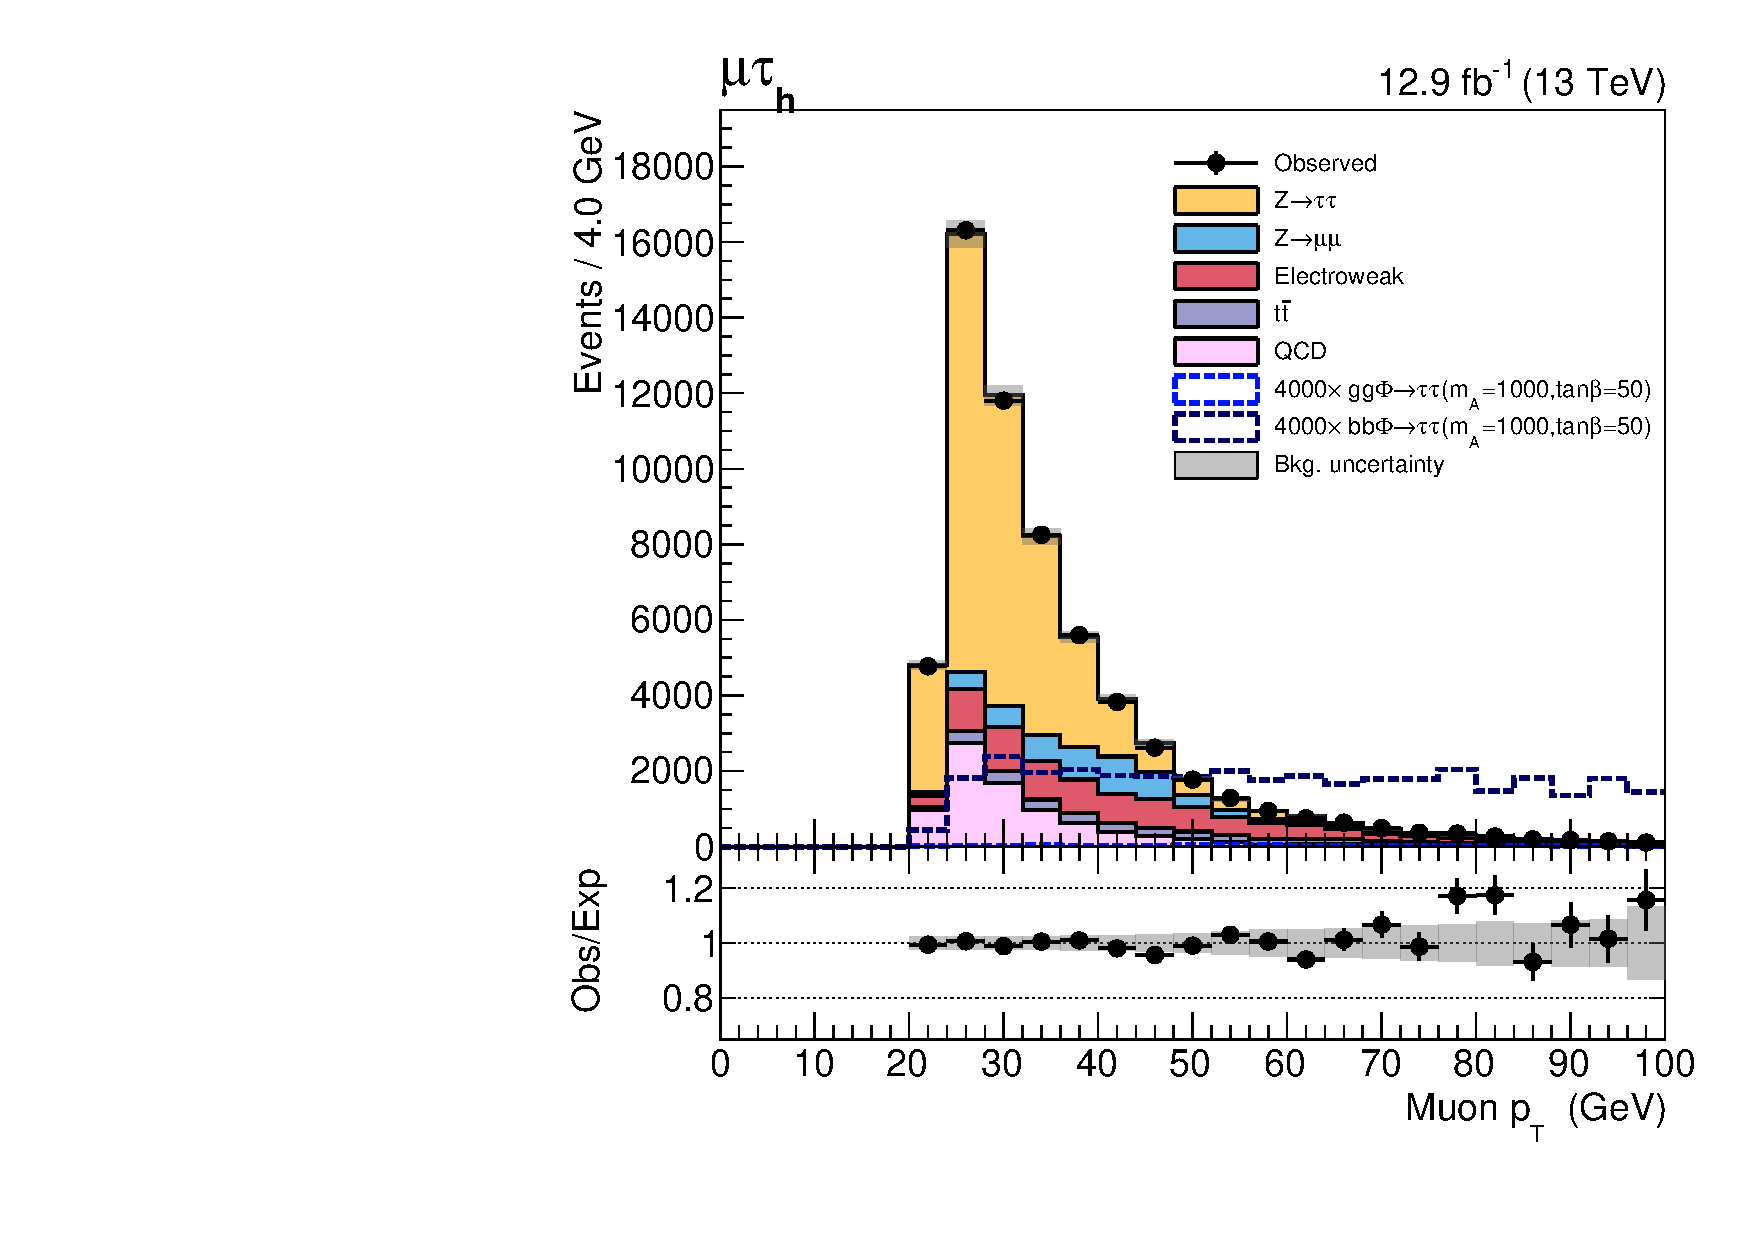
\includegraphics[width=0.5\textwidth]{./MSSM/Figures/pt_1_inclusive_mt_2016.pdf}}
\subfloat[Electron $\eta$]{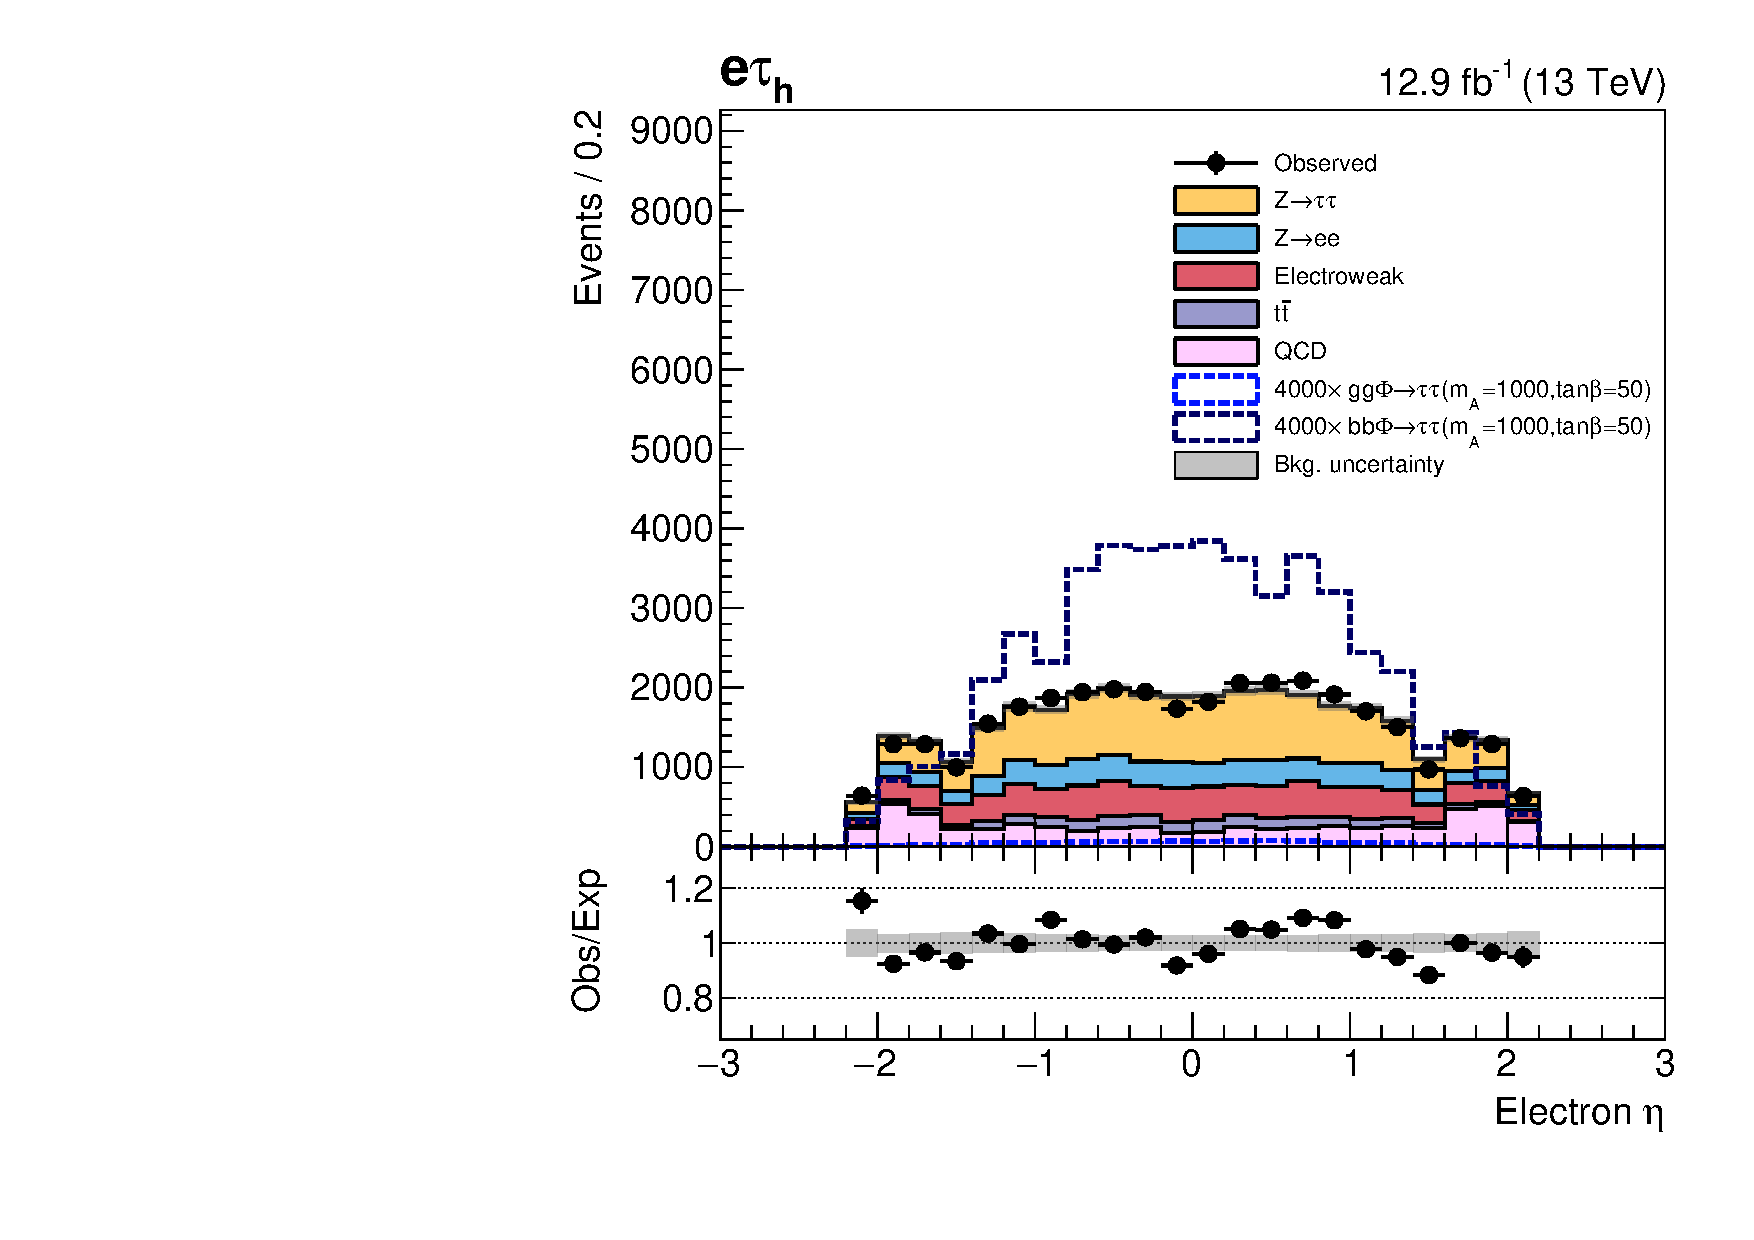
\includegraphics[width=0.5\textwidth]{./MSSM/Figures/eta_1_inclusive_et_2016.pdf}}
\end{center}
\caption[The \pT~of the muon in the \mutau channel
and $\eta$ of the electron in the \etau channel, with the signal
overlaid.]{(a) \pT~of the muon in the \mutau channel and (b) $\eta$ of the electron in the \etau channel.
The gluon fusion (dashed blue line)
and b-associated (dashed purple line) signals are overlaid. The signals are normalised to 4000 times their
cross-section times branching ratio at \mA=1 TeV and \tanb=50 in the $m_{h}^{\text{mod+}}$ scenario.}
\label{fig:mt_muonpt}
\end{figure}
 
\subsection{Pair selection and vetos}
\label{sec:mssm_eventsel_pairs}
After applying trigger
requirements, identification criteria and kinematic cuts
more than one possible candidate pair can exist. If
this is the case the pair with the two most isolated candidates
 is chosen, as isolated candidates are less likely 
to be jets misreconstructed
as leptons or hadronic taus.
%If this
%is the case for an event, the pair is chosen as follows:
%\begin{itemize}
%\setlength{\itemsep}{-\baselineskip}
%\item Prefer the pair with most isolated candidate 1 (muon for \mutau and \emu channels,
%electron for \etau channel, either of the $\Pgt_h$s in \tautau channel). For electrons
%and muons this means the object with the smallest relative isolation value is preferred, for $\Pgt_h$s the
%object with raw MVA isolation value nearest to 1.
%\item If the isolation of candidate 1 is the same in both pairs, prefer the pair with highest candidate 1 \pT.
%\item If the \pT~of candidate 1 is the same in both pairs, prefer the pair with most isolated
%candidate 2 (e for the \emu channel, the other $\Pgt_h$ for the \tautau channel, 
%and the $\Pgt_h$ for \etau and \mutau channels).
%\item If the isolation of candidate 2 is the same in both pairs, prefer the pair with highest candidate 2 \pT.
%\end{itemize}

To prevent overlap with other channels, events are rejected
if there are muons and electrons, other than those in the selected pair,
with \pT~$>10$ GeV and passing loose ID and isolation requirements.
This also reduces backgrounds from \WZ events. The application
of these vetos means that the selection of the pair with the
two most isolated candidates is only important where hadronic
taus are concerned, for if there were additional electrons (muons)
the event would not pass the electron (muon) veto.
In addition to these extra electron and muon vetos, \Zee events are 
reduced in the \etau channel by rejecting events
where an opposite--sign pair of electrons of \pT~$>15$ GeV
and passing very loose ID and isolation requirements can be formed. 
In the \mutau channel the contribution from \Zmm events
is reduced in a similar fashion. 

\subsection{\texorpdfstring{Event selection in the \mutau channel}{Event selection in the mu tau channel}}
\label{sec:mssm_eventsel_mt}
The trigger only requires a muon at \ac{L1}, while at the level of the \ac{HLT}
loose identification and isolation criteria are applied to this muon.

The offline event selection requires an oppositely charged
muon and hadronically decaying tau, which are well--separated ($\Delta R > 0.5$).
The minimum \pT~of the muon is required to be 23 GeV, with $|\eta| < 2.1$. %due to trigger conditions
Additional ``medium'' identification requirements are placed on the muon, and the impact
parameters of the muon must satisfy $d_{xy}<0.045$ cm and $d_{z}<0.2$ cm. The muon is also
required to be isolated, with $I_{\text{rel}}^{\mu}<0.15$, where the isolation variable
is calculated using a cone size of $\Delta R = 0.4$.

The hadronic tau needs to have a \pT~greater than 30 GeV, $|\eta|<2.3$,
is required to be reconstructed by the HPS algorithm and to pass the medium
working point of the MVA isolation discriminator. The impact parameter $d_{z}$ is
required to be less than 0.2 cm. Finally the hadronic tau is required
to satisfy the very loose working point of the anti--electron discriminator
and the tight working point of the anti--muon discriminator.

The selection on the muon's relative isolation is chosen after comparing
the performance of several isolation variables, using different relative isolation selections.
This was based on a simple \mutau channel
event selection as described above, only varying the isolation requirements.
The selection was optimised based on two figures of merit, both of
which consider \Ztautau as the signal and the other backgrounds
as background. The first figure of merit used is the number of signal events divided by the
square root of the number of background events, $S/\sqrt{B}$, after
the selection. The aim with this figure of merit is to choose
the isolation selection that maximises it. The second figure of merit
is the uncertainty interval on the best-fit value for a maximum--likelihood fit
to the \Ztautau signal strength, which should be minimised by the choice of
isolation selection.

The isolation variables studied include
the $\Delta\beta$ corrected isolation variable analogous
to the one given for electrons in equation \ref{eqn:electron_reliso} with 
isolation cone sizes of $\Delta R$  0.3 and 0.4. In addition
to this a very similar
variable, which does not just consider charged \ac{PF} hadrons but
also electrons and muons in the isolation sum, is considered. This
variable is also studied for cone sizes of 0.3 and 0.4. Finally,
a relative isolation variable based solely on the \pT~of tracks from the primary
vertex,
\begin{equation}\label{eqn:reltrkiso}
I_{\text{trk}} = \frac{\Sigma p_{\text{T}}^{\text{tracks from PV within cone of 0.3 of the muon}}}{p_{\text{T}}^{\mu}}, \end{equation} 
is studied. The $S/\sqrt{B}$ for the different isolation variables is shown in figure \ref{fig:mssm_selection_mt_muons}a, with the
size of the error interval from the maximum--likelihood fit to the \Ztautau signal strength shown in 
\ref{fig:mssm_selection_mt_muons}b. As both figures of merit do not
change so much with varying isolation requirements we can see that this analysis
is not so sensitive to fake, nonisolated muons. The choice of isolation variable is therefore
driven mostly by simplicity and consistency with other \ac{CMS} analyses.

\begin{figure}[h!]
\begin{center}
\subfloat[$S/\sqrt{B}$]{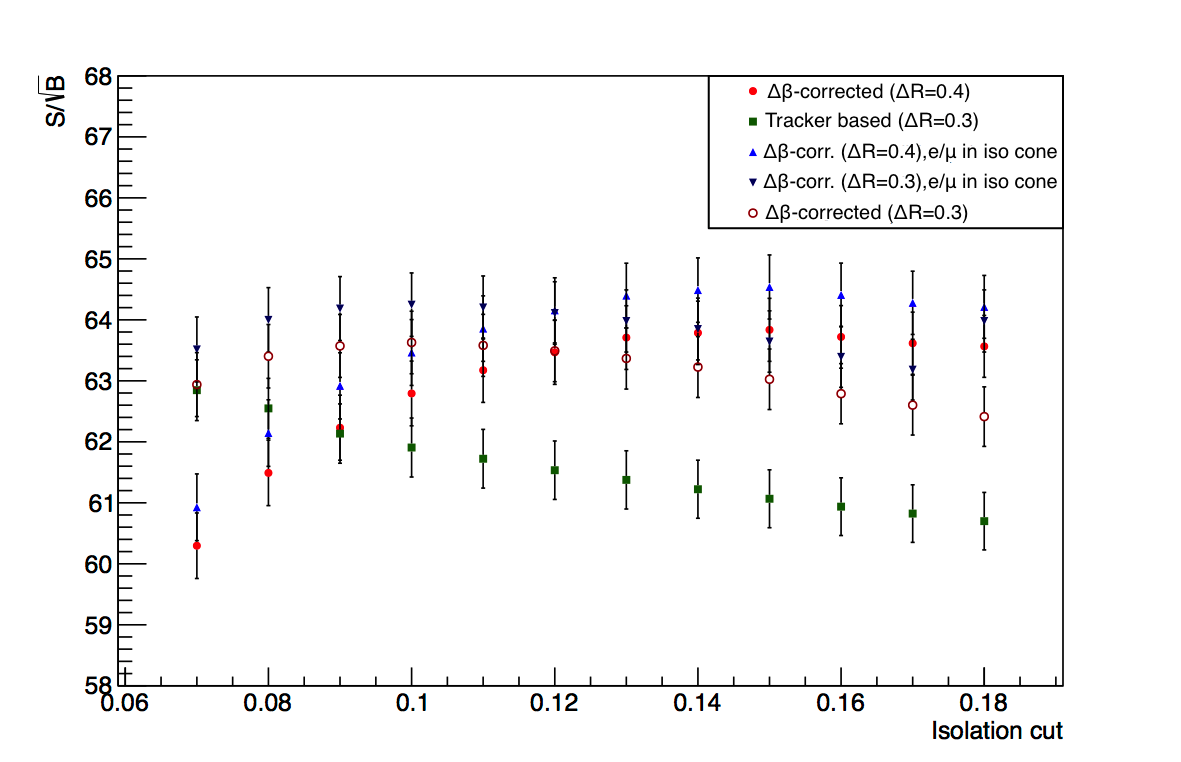
\includegraphics[width=0.7\textwidth]{./MSSM/Figures/s_over_root_b_mt_m.png}}~\\
\subfloat[Size of error interval]{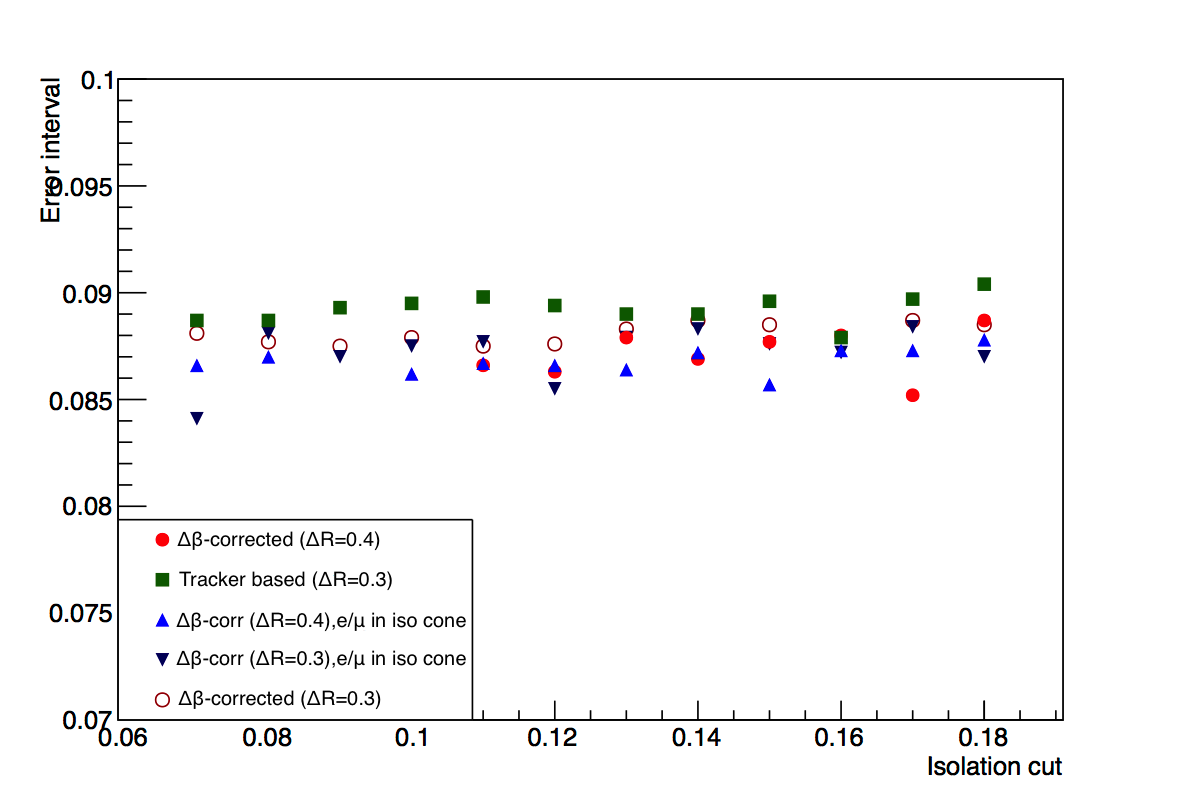
\includegraphics[width=0.7\textwidth]{./MSSM/Figures/mt_muons_iso_errint.png}}
\end{center}
\caption[The $S/\sqrt{B}$ for \Ztautau signal and
the size of the error interval on the best--fit value of a
maximum--likelihood fit to the \Ztautau signal strength, for various 
isolation selections.]{(a) The $S/\sqrt{B}$ for \Ztautau signal and (b) the size of the error interval on 
the best--fit value of a maximum--likelihood fit to the \Ztautau signal strength,
for various selections of the $\Delta\beta$--corrected
isolation variable with a cone size of $\Delta R = 0.4$ (solid circles), 
the $\Delta\beta$--corrected isolation variable with a cone size of $\Delta R = 0.3$ (open circles),
the $\Delta\beta$--corrected isolation variable including electrons and muons in the isolation
sum, for a cone size of $\Delta R =0.4$ (upward facing triangles) and $\Delta R =0.3$ (downward facing triangles) and
the tracker--based relative isolation (solid squares).}
\label{fig:mssm_selection_mt_muons}
\end{figure}

A topological selection on the \mT~variable, 
introduced in section \ref{sec:hhh_selection_categories}, is made on 
events in the \mutau channel. This selection and the
choice of hadronic tau isolation working point provide two competing
effects and therefore they are optimised in a 2D--optimisation. 
The pre--fit expected upper limits on $\sigma\times$BR for both gg$\phi$ and bb$\phi$
production with decay into $\Pgt\Pgt$ at several mass points 
in the 90 GeV -- 3.2 TeV range are used as a figure of merit.
Because of the use of such a wide range of signal masses, it
is not possible to choose a selection that is optimal
for every mass point. This is illustrated in figure \ref{fig:mssm_selection_mt_taumt}:
figure \ref{fig:mssm_selection_mt_taumt}a shows the upper limit on $\sigma\times$BR for
the gluon fusion production process, for a mass $m_{\phi} = 160$ GeV, with
figure \ref{fig:mssm_selection_mt_taumt}b showing this upper limit for $m_{\phi} = 2.9$ TeV.
Figure \ref{fig:mssm_gradcuts_mt} shows the effect of gradually loosening the \mT~and hadronic
tau isolation working point selection on both the gg$\phi$ and bb$\phi$ production processes. 

\begin{figure}[h!]
\begin{center}
\subfloat[$m_{\phi} = 160$ GeV]{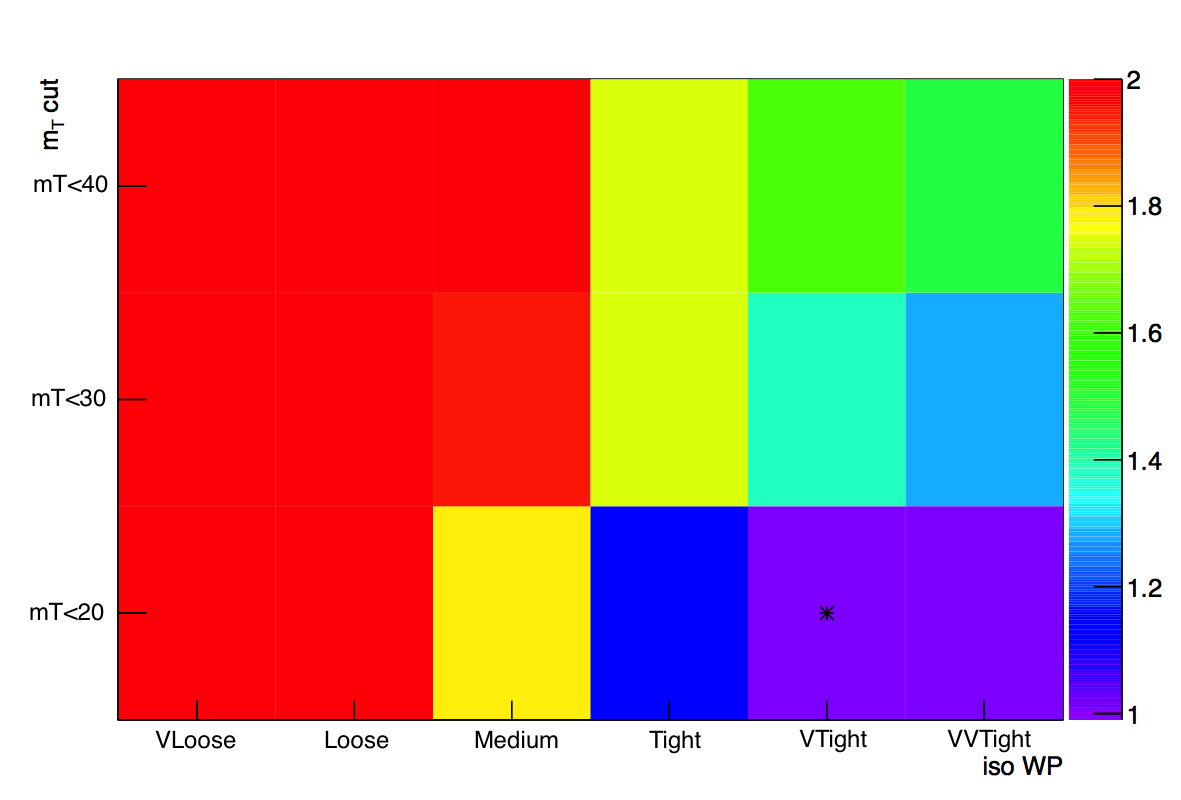
\includegraphics[width=0.5\textwidth]{./MSSM/Figures/optimisation_ggh_mt_160_range12.png}}
\subfloat[$m_{\phi} = 2.9$ TeV]{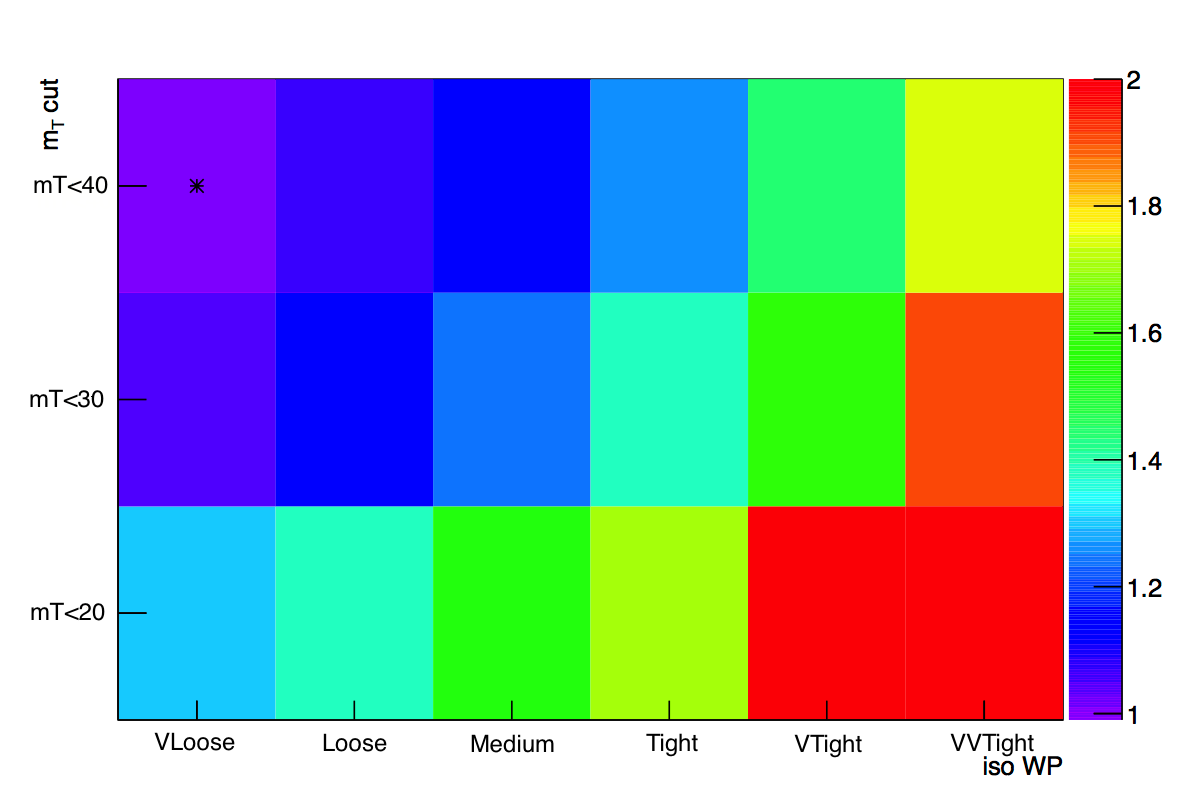
\includegraphics[width=0.5\textwidth]{./MSSM/Figures/optimisation_ggh_mt_2900_range12.png}}
%\subfloat[$m_{\phi} = 1600$ GeV]{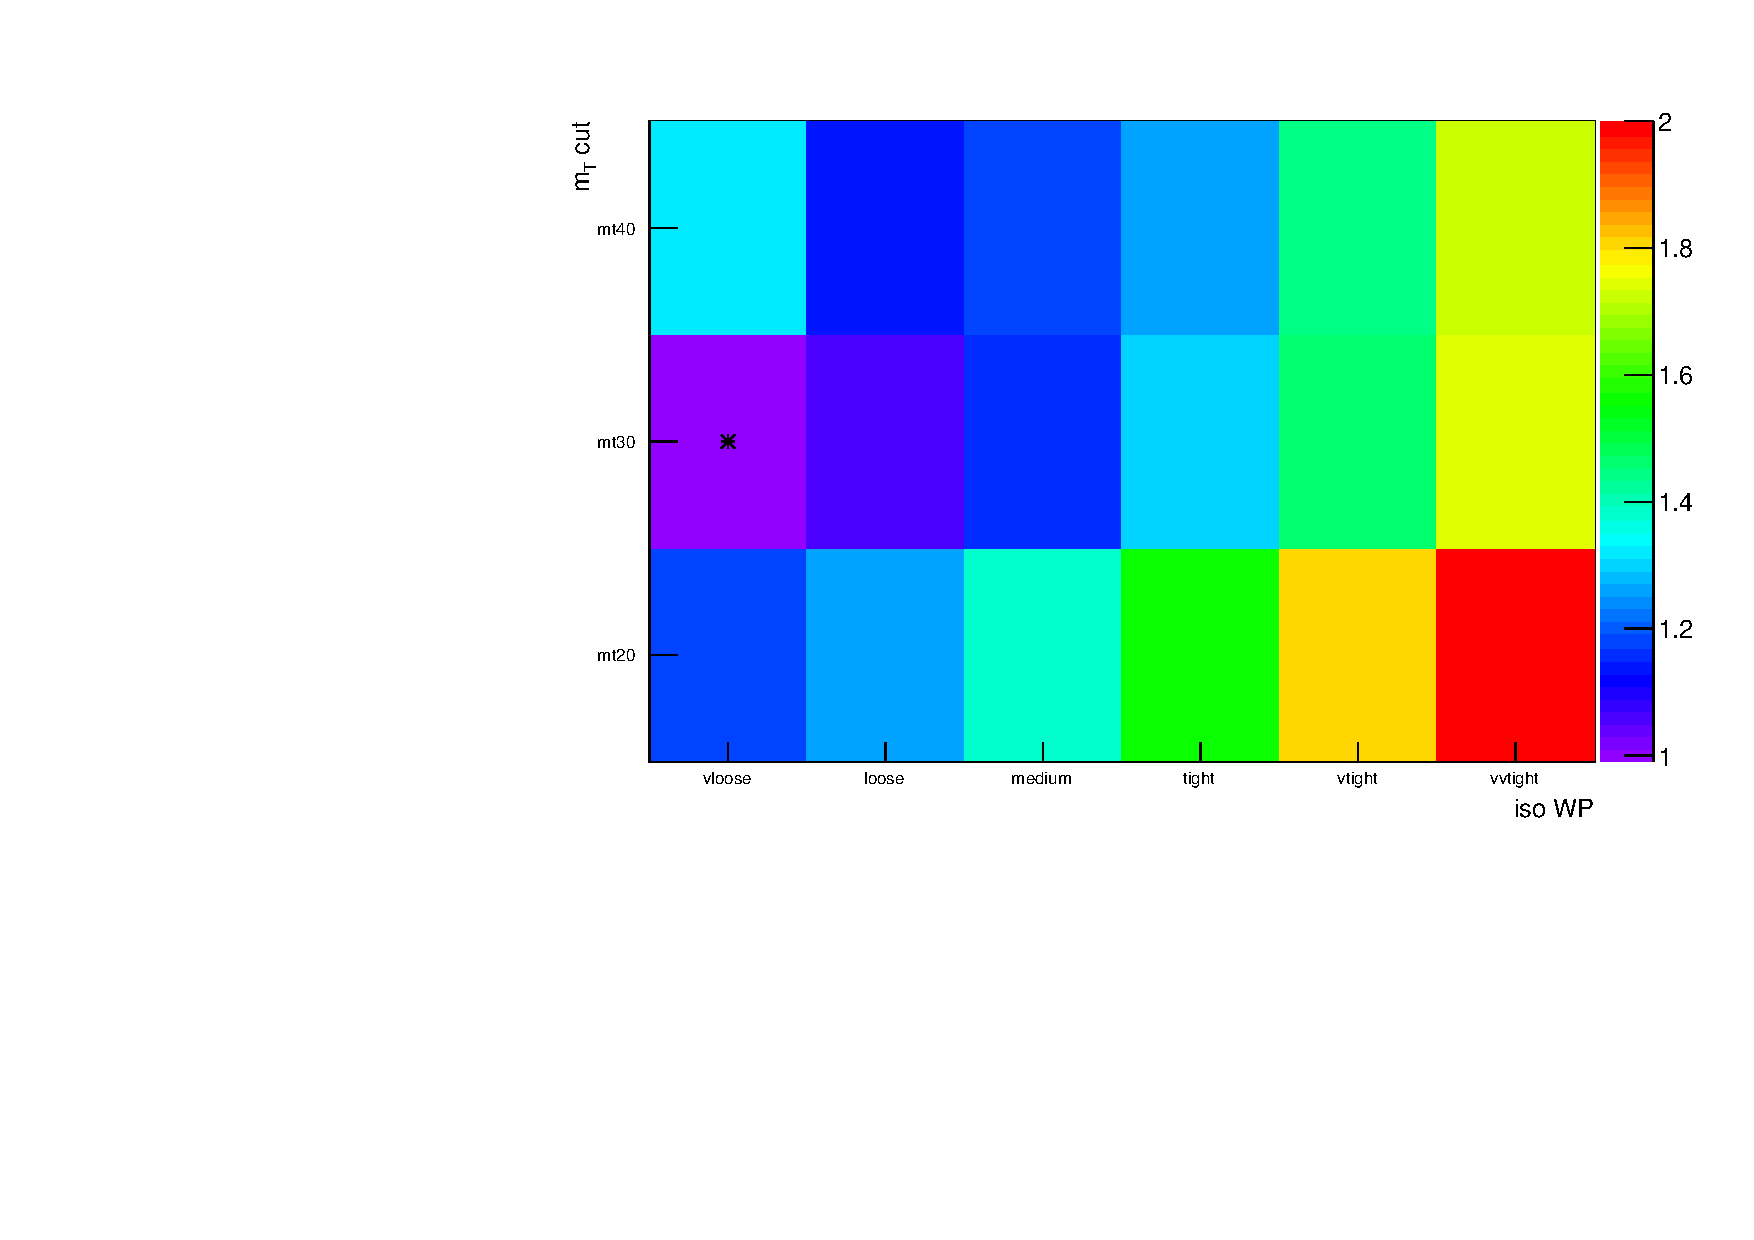
\includegraphics[width=0.5\textwidth]{./MSSM/Figures/optimisation_ggh_mt_1600_range12.pdf}}
%\subfloat[$m_{\phi} = 2900$ GeV]{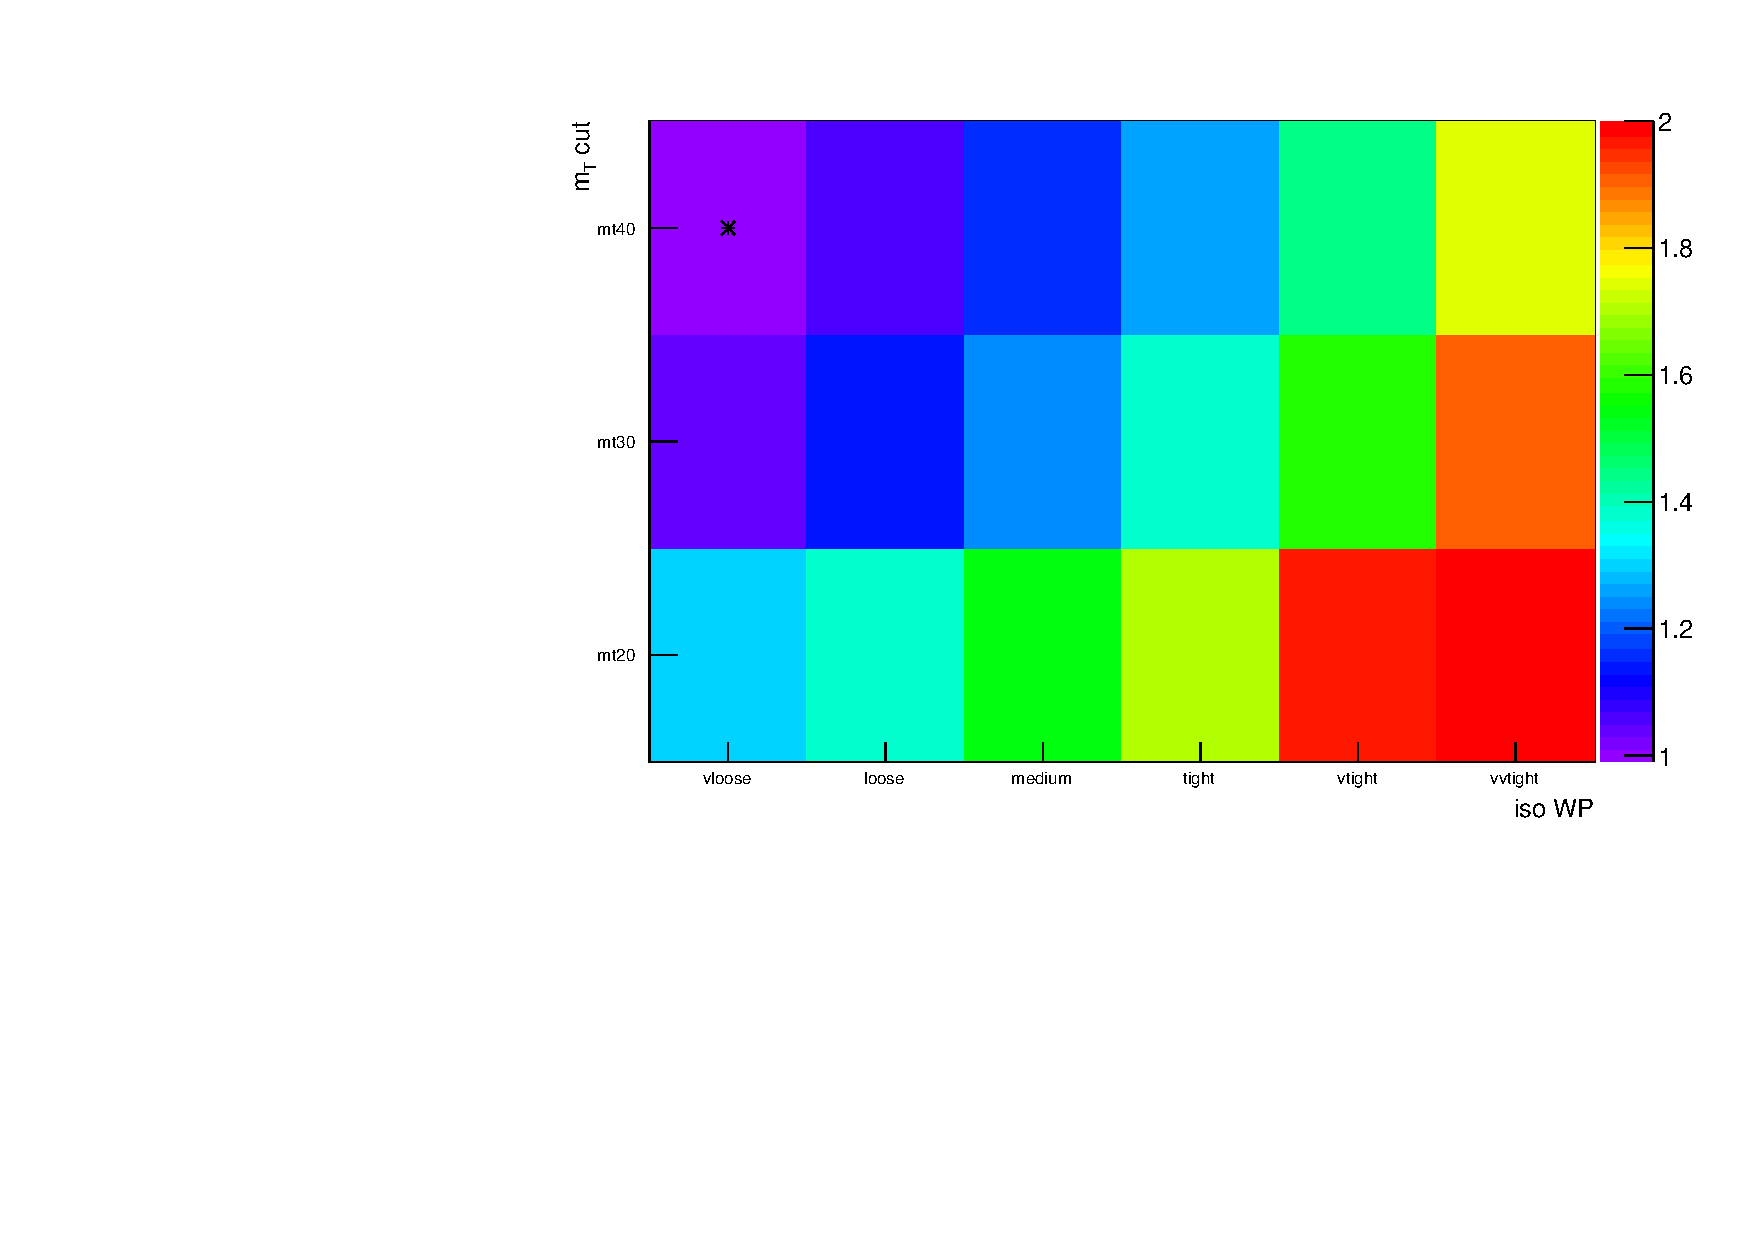
\includegraphics[width=0.5\textwidth]{./MSSM/Figures/optimisation_ggh_mt_2900_range12.pdf}}
\end{center}
\caption[Pre--fit expected limit on $\sigma\times$BR for the gg$\phi$
production process with decay into $\Pgt\Pgt$ as a function of tau isolation 
working point and \mT~selection, for two mass points.]{Pre--fit expected limit on $\sigma\times$BR for the gg$\phi$ production process with decay into $\Pgt\Pgt$,
as a function of tau isolation working point (from very loose to very very tight) and
of \mT~selection from \mT$<20$ GeV to \mT$<40$ GeV, normalised to the best limit in the plane, indicated by the asterisk. This is shown
for (a) $m_{\phi}$ = 160 GeV and (b) $m_{\phi}$ = 2.9 TeV. The most optimal combination of \mT~selection and 
hadronic tau isolation working point varies, with looser selections preferred at higher mass.}
\label{fig:mssm_selection_mt_taumt}
\end{figure}
~
\begin{figure}[h!]
\begin{center}
\subfloat[gg$\phi$]{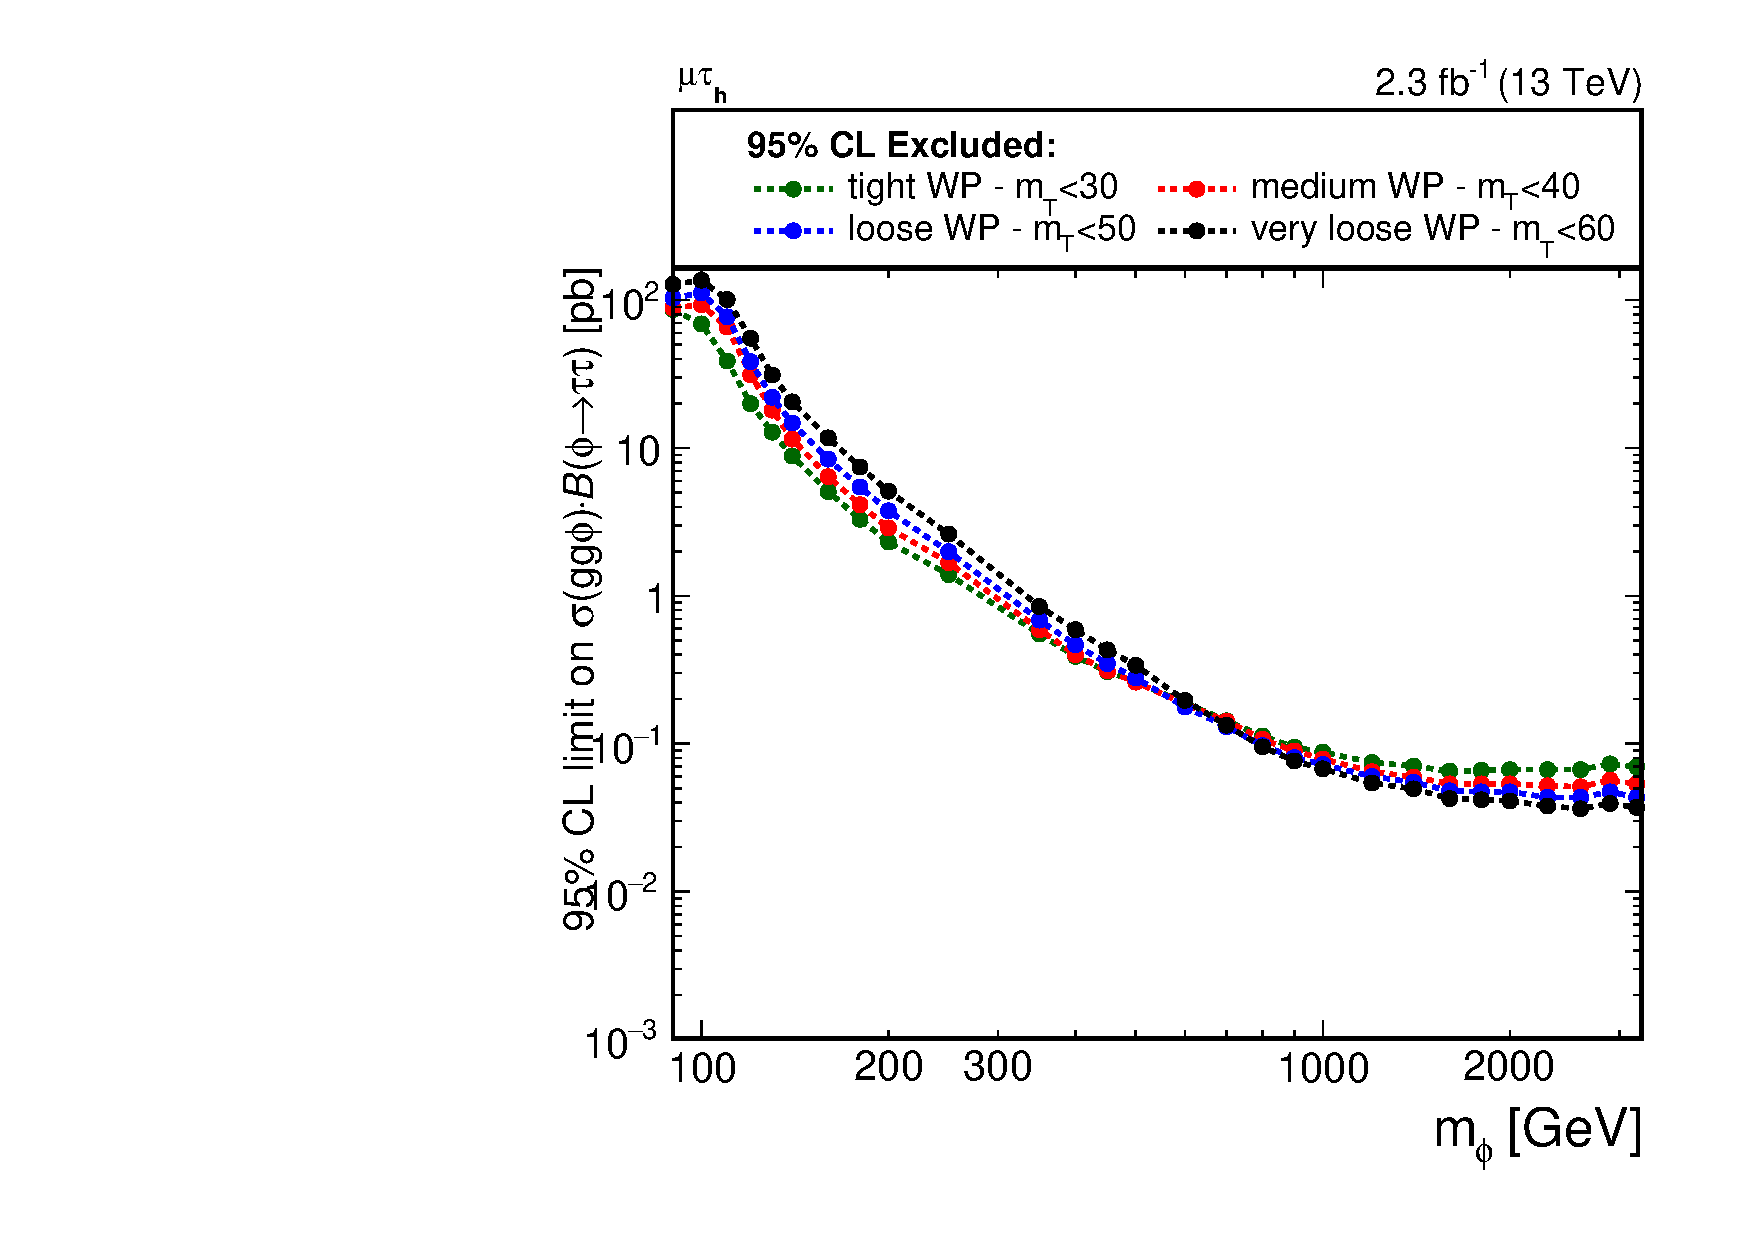
\includegraphics[width=0.5\textwidth]{./MSSM/Figures/mssm_gradcuts_ggH_mt.pdf}}
\subfloat[bb$\phi$]{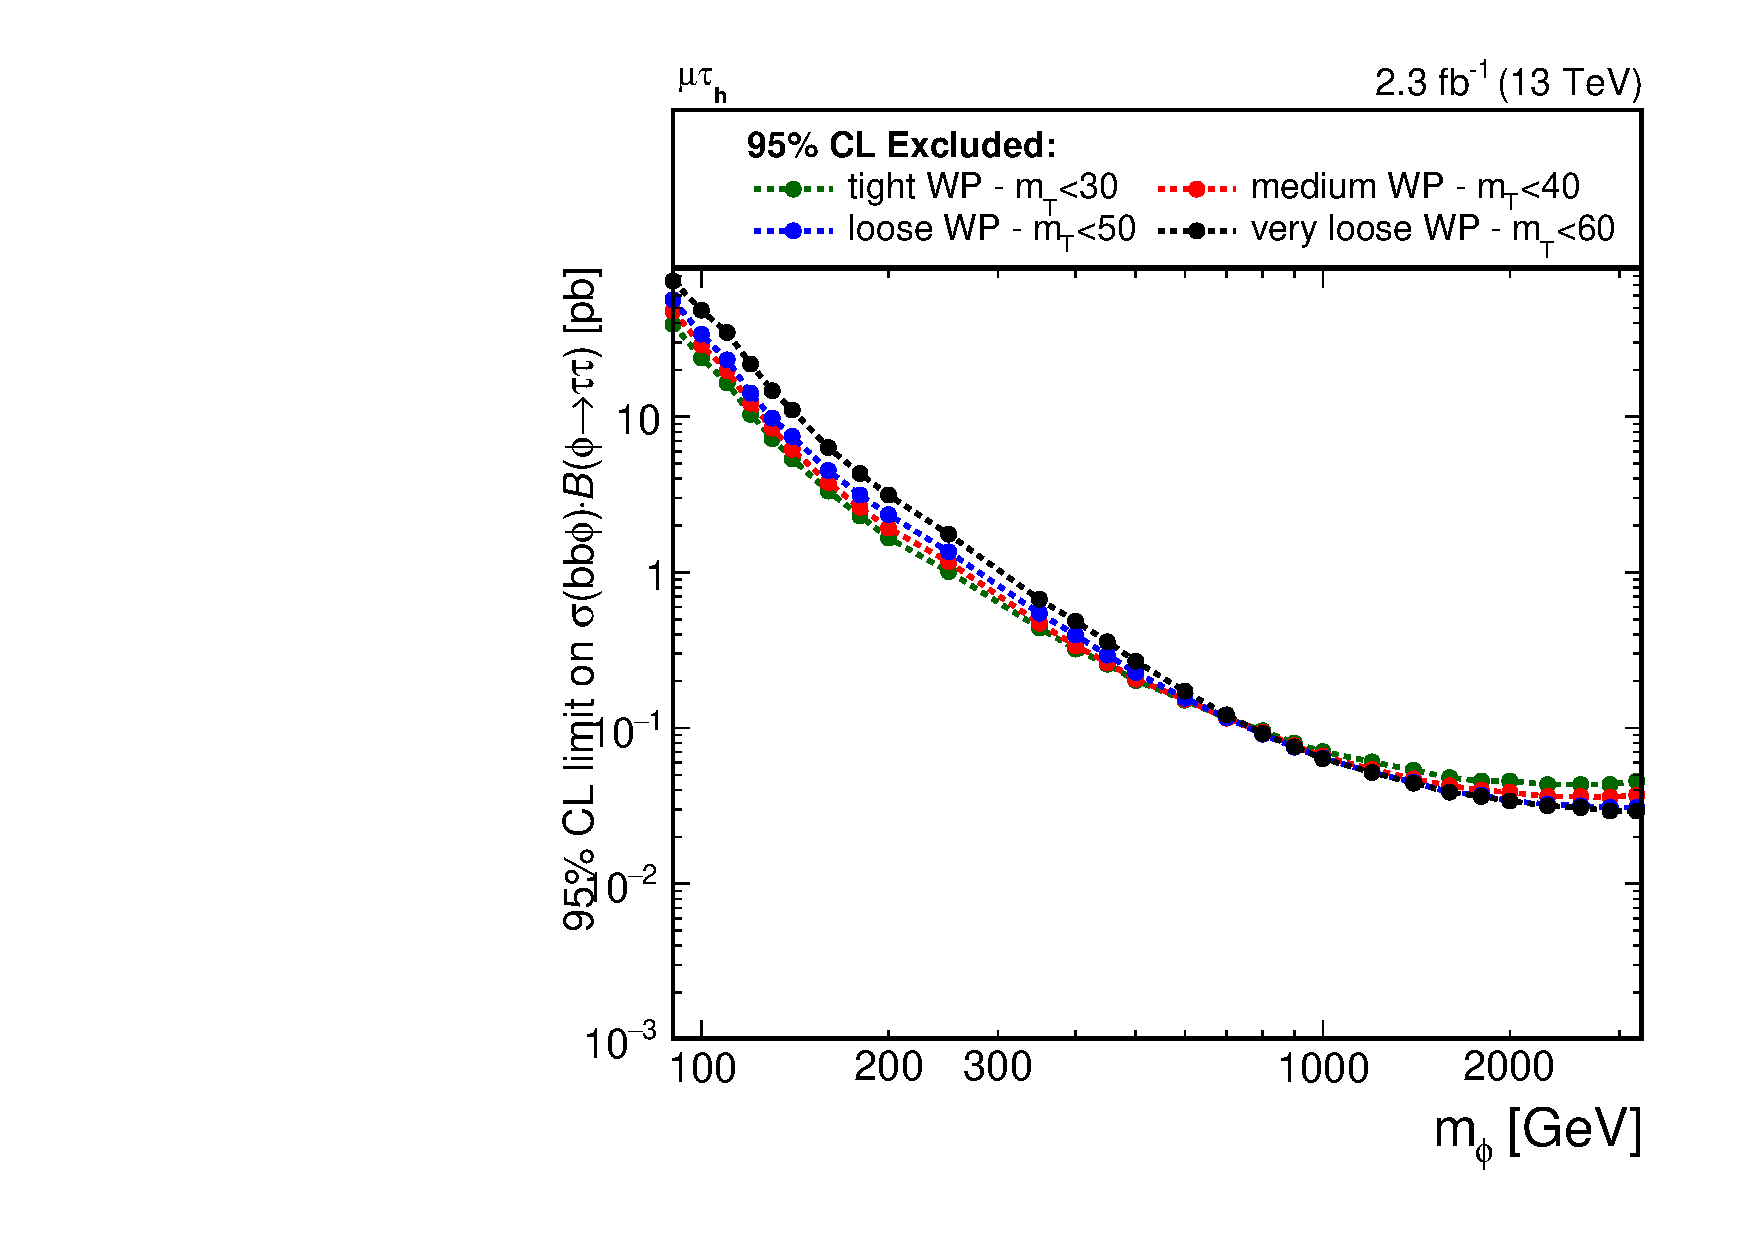
\includegraphics[width=0.5\textwidth]{./MSSM/Figures/mssm_gradcuts_bbH_mt.pdf}}
\end{center}
\caption[Pre-fit expected limits on $\sigma \times$ BR for the gg$\phi$ and bb$\phi$
processes
in the
\mutau channel for an increasingly looser \mT~selection and tau isolation
working point.]{Pre-fit expected limits on $\sigma \times$ BR in the \mutau channel for (a) gg$\phi$ and
(b) bb$\phi$ production, for an increasingly looser \mT~selection and tau isolation working point, starting
at the tight working point and \mT$<30$ GeV in green, the medium working point and \mT$<40$ GeV in red,
the loose working point and \mT$<50$ GeV in blue and the very loose working point and \mT$<60$ GeV in black. Loosening
the tau isolation working point and \mT~selection gradually improves limits at higher mass, and
degrades them at low mass.}
\label{fig:mssm_gradcuts_mt}
\end{figure}

From these figures
we observe that looser selections are preferred for higher masses. This behaviour can be
explained by considering the function of each of the selections. Tightening the hadronic
tau isolation working point reduces the selection of fake taus and increases the proportion
of backgrounds which contain real hadronic taus. The \mT~selection reduces
the \Wjets background. As the backgrounds are concentrated at the lower
end of the spectrum of mass--like discriminating variables, such tighter
selections are preferred where signal and backgrounds overlap. For higher masses the
backgrounds are lower in the region where the signal peaks,
and there is more benefit to loosening the selection
to increase the signal efficiency than to keep the tighter selection
to reduce an already low background.
The selection was optimised for masses around 800 GeV - 1 TeV, by
using the medium hadronic tau isolation working point and a selection on \mT$<40$ GeV.

The choice of the hadronic tau \pT~selection is driven by the effect on the low mass region:
raising the \pT~selection by 10 GeV from the minimum of 20 GeV does not affect the sensivity
of the analysis for high mass points, while recovering some of the loss of loosening 
tau isolation working point and \mT~cut. The reason for this is that when using \pT$>30$ GeV 
fewer background events are selected. The effect of the increased hadronic tau \pT~selection on the 
upper limits for the gg$\phi$ production process is shown
in figure \ref{fig:mssm_tauptcut}a, and on the bb$\phi$ production process
in figure \ref{fig:mssm_tauptcut}b. At low mass the improvement in the gg$\phi$ limits
obtained by increasing the \pT~selection is sizeable, for bb$\phi$ events the effect is much
less pronounced.

\begin{figure}[h!]
\begin{center}
\subfloat[gg$\phi$]{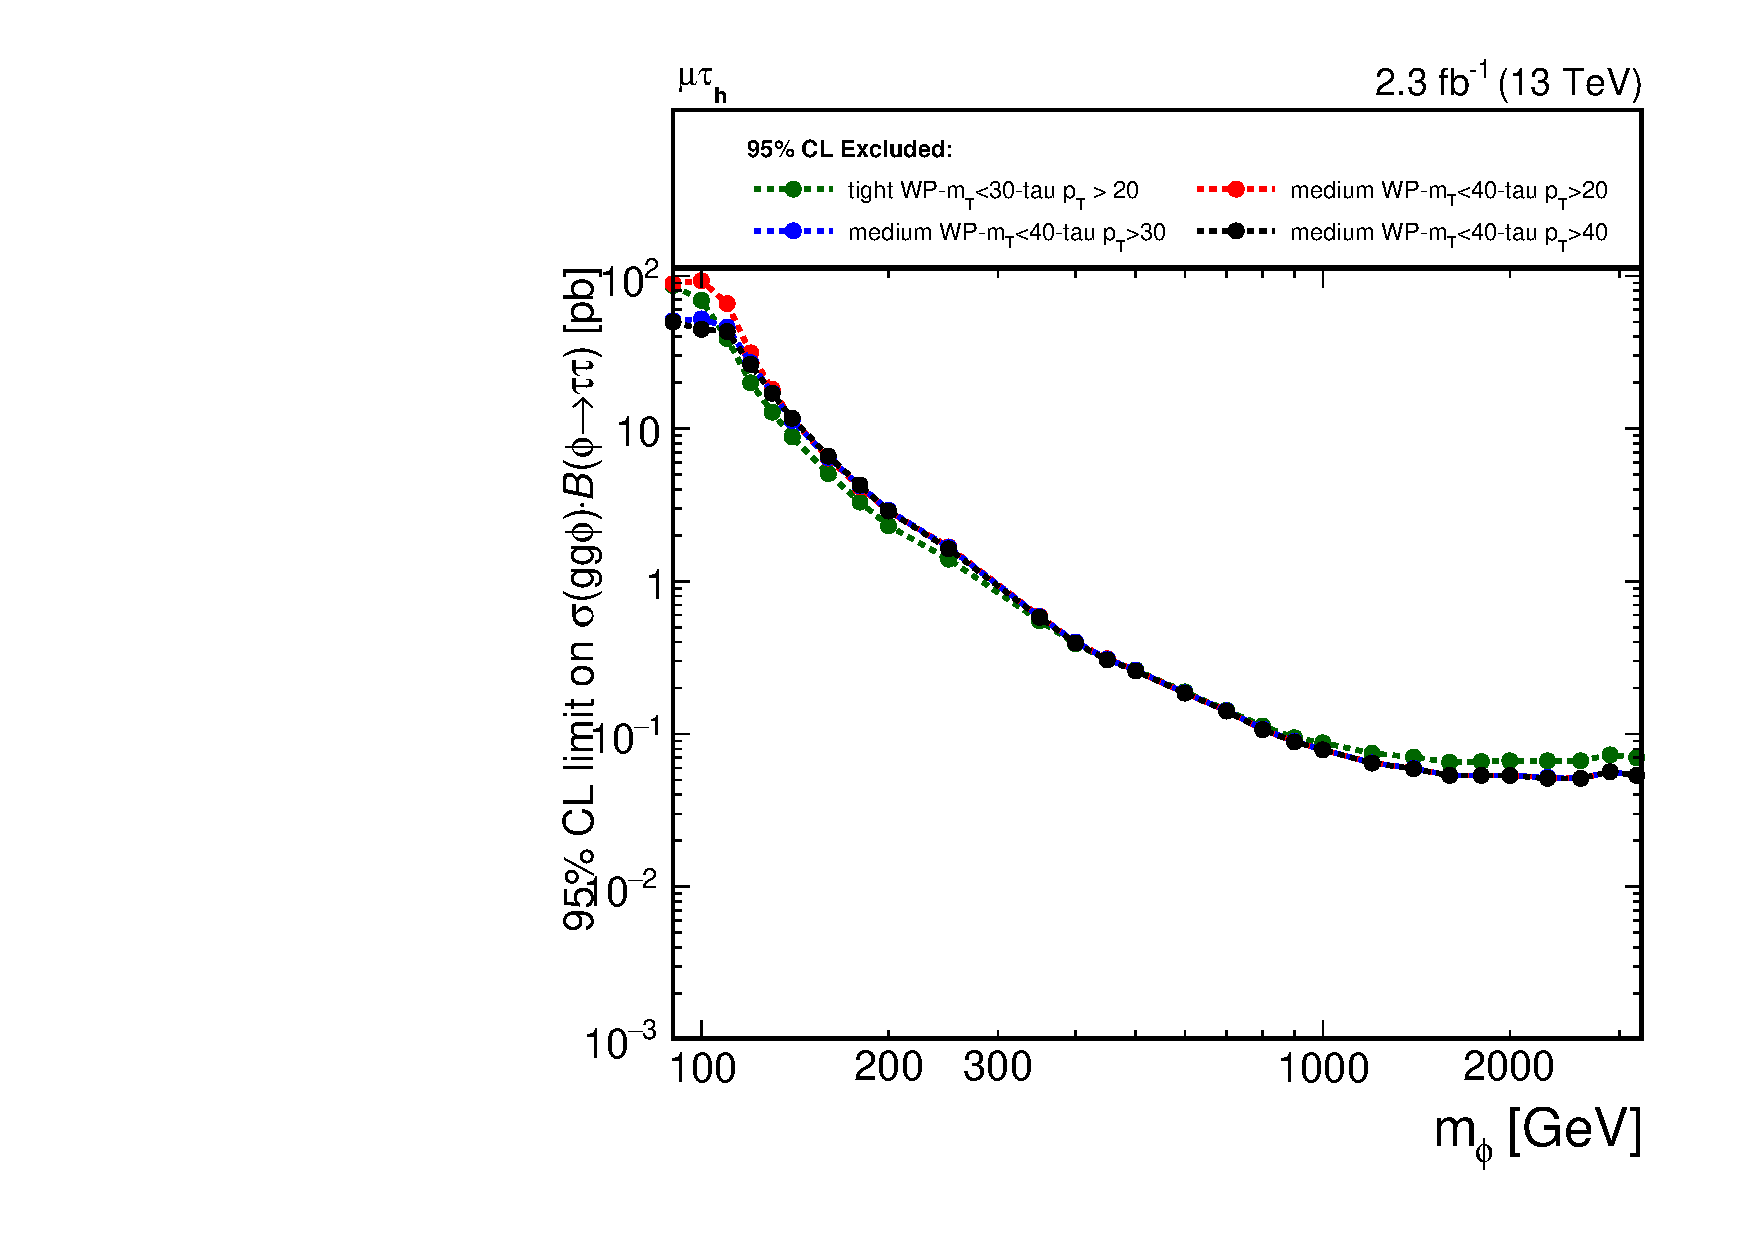
\includegraphics[width=0.5\textwidth]{./MSSM/Figures/mssm_optimisation_mediummt40_vs_tightmt30pt20_mt_ggH_remake.pdf}}
\subfloat[bb$\phi$]{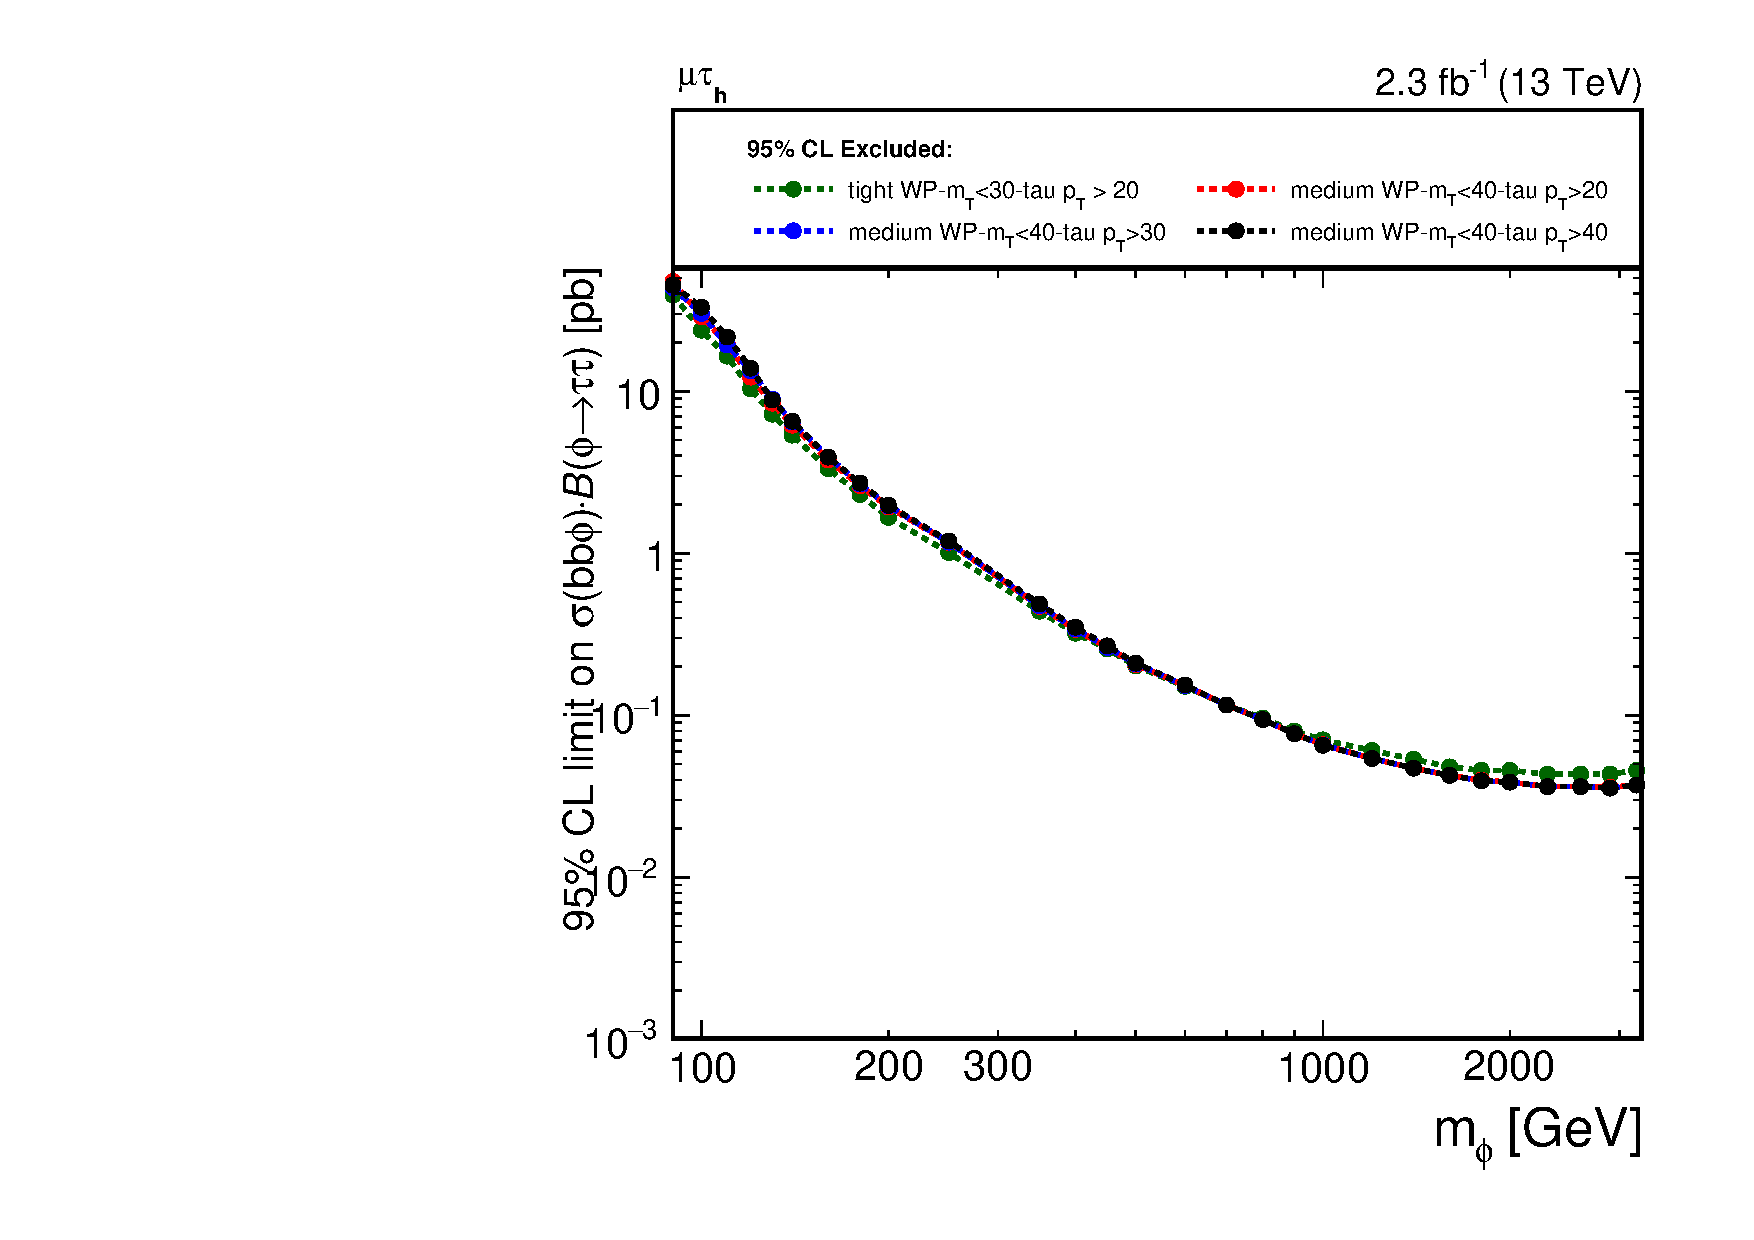
\includegraphics[width=0.5\textwidth]{./MSSM/Figures/mssm_optimisation_mediummt40_vs_tightmt30pt20_mt_bbH_remake.pdf}}
\end{center}
\caption[Pre-fit expected limits on $\sigma\times$BR in the
\mutau channel for gg$\phi$ and bb$\phi$ prouduction, comparing
different hadronic tau \pT~cuts.]{Pre-fit expected limits on $\sigma\times$BR in the \mutau channel for (a) gg$\phi$ production and (b) bb$\phi$ production. The
limits when using the medium hadronic tau isolation working point and \mT$<40$ GeV selection using a minimum
hadronic tau \pT~selection of 20 GeV (red circles), 30 GeV (blue circles) and 40 GeV (black circles) are shown. The green
circles show the limits using tighter tau isolation working point and \mT~selection. The limits on
the gg$\phi$ production process improve at low masses when increasing the minimum hadronic tau \pT~selection,
the effect on the bb$\phi$ production process is less pronounced.}
\label{fig:mssm_tauptcut}
\end{figure}

\subsection{\texorpdfstring{Event selection in the \etau channel}{Event selection in the e tau channel}}
\label{sec:mssm_eventsel_et}
For selection of events in the \etau channel, the first step is
a trigger that only requires an electron at \ac{L1}. Loose ID and isolation
criteria are made on the electron with the \ac{HLT}.

The offline event selection requires an oppositely charged
electron and hadronically decaying tau, which are well--separated ($\Delta R > 0.5$).
The minimum \pT~of the electron is required to be 26 GeV, with $|\eta| < 2.1$. %due to trigger conditions
The impact parameters of the electron are required to satisfy
$d_{xy} < 0.045$ cm and $d_{z} < 0.2$ cm, and the electron
must pass additional identification criteria. The working point of the
MVA identification discriminator that is used corresponds to a cut on the discriminator
which selects electrons from \Zee events with 80\% efficiency. In addition the
electron needs to be isolated, $I_{\text{rel}}^{\Pe} < 0.1$, with the relative isolation variable calculated with a cone size of 0.3.

The hadronic tau is required to have a \pT~greater than 30 GeV, $|\eta|<2.3$,
and is required to be reconstructed by the HPS algorithm and to pass the medium
working point of the MVA isolation discriminator. The impact parameter $d_{z}$ of the
hadronic tau must be less than 0.2 cm.
Finally, the hadronic tau must 
pass the tight working point of the anti--electron discriminator
and the loose working point of the anti--muon discriminator.

Analogously to the muons, it was found that the analysis is not highly sensitive
to the choice of electron isolation variable and cut value.
A topological selection on the \mT~variable is also made in this channel to reject \Wjets events. 
The value of \mT~$< 50$ GeV that is used is obtained by performing a 2D optimisation where the \mT~selection
and hadronic tau isolation working point are varied at the same time. The same considerations as
for the \mutau channel apply, as illustrated in figure \ref{fig:mssm_gradcuts_et}.
The choice of the hadronic tau \pT~selection of 30 GeV is
made to recover some of the sensitivity lost at low mass by using looser \mT~and hadronic
tau isolation criteria. This is illustrated in figure \ref{fig:mssm_tauptcut_et}.

\begin{figure}[h!]
\begin{center}
\subfloat[gg$\phi$]{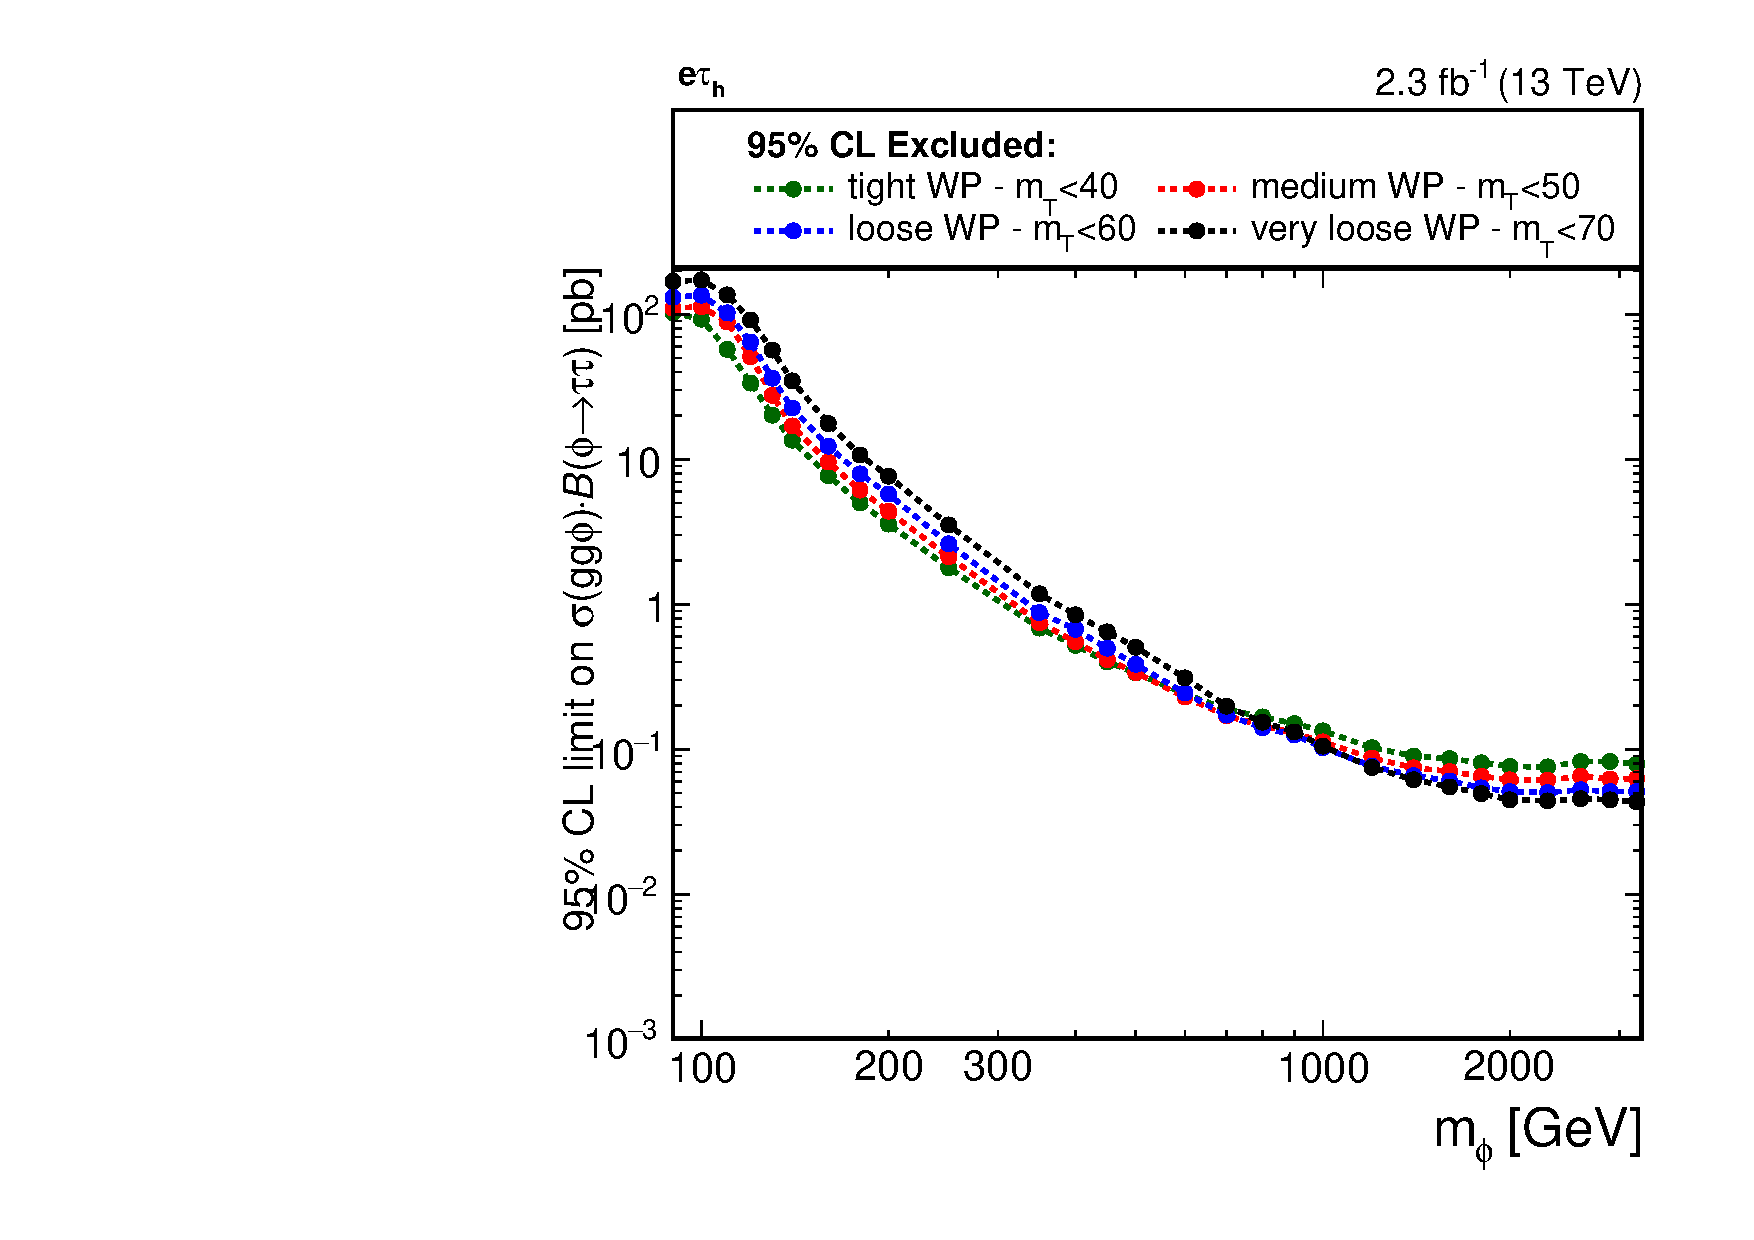
\includegraphics[width=0.5\textwidth]{./MSSM/Figures/mssm_gradcuts_ggH_et.pdf}}
\subfloat[bb$\phi$]{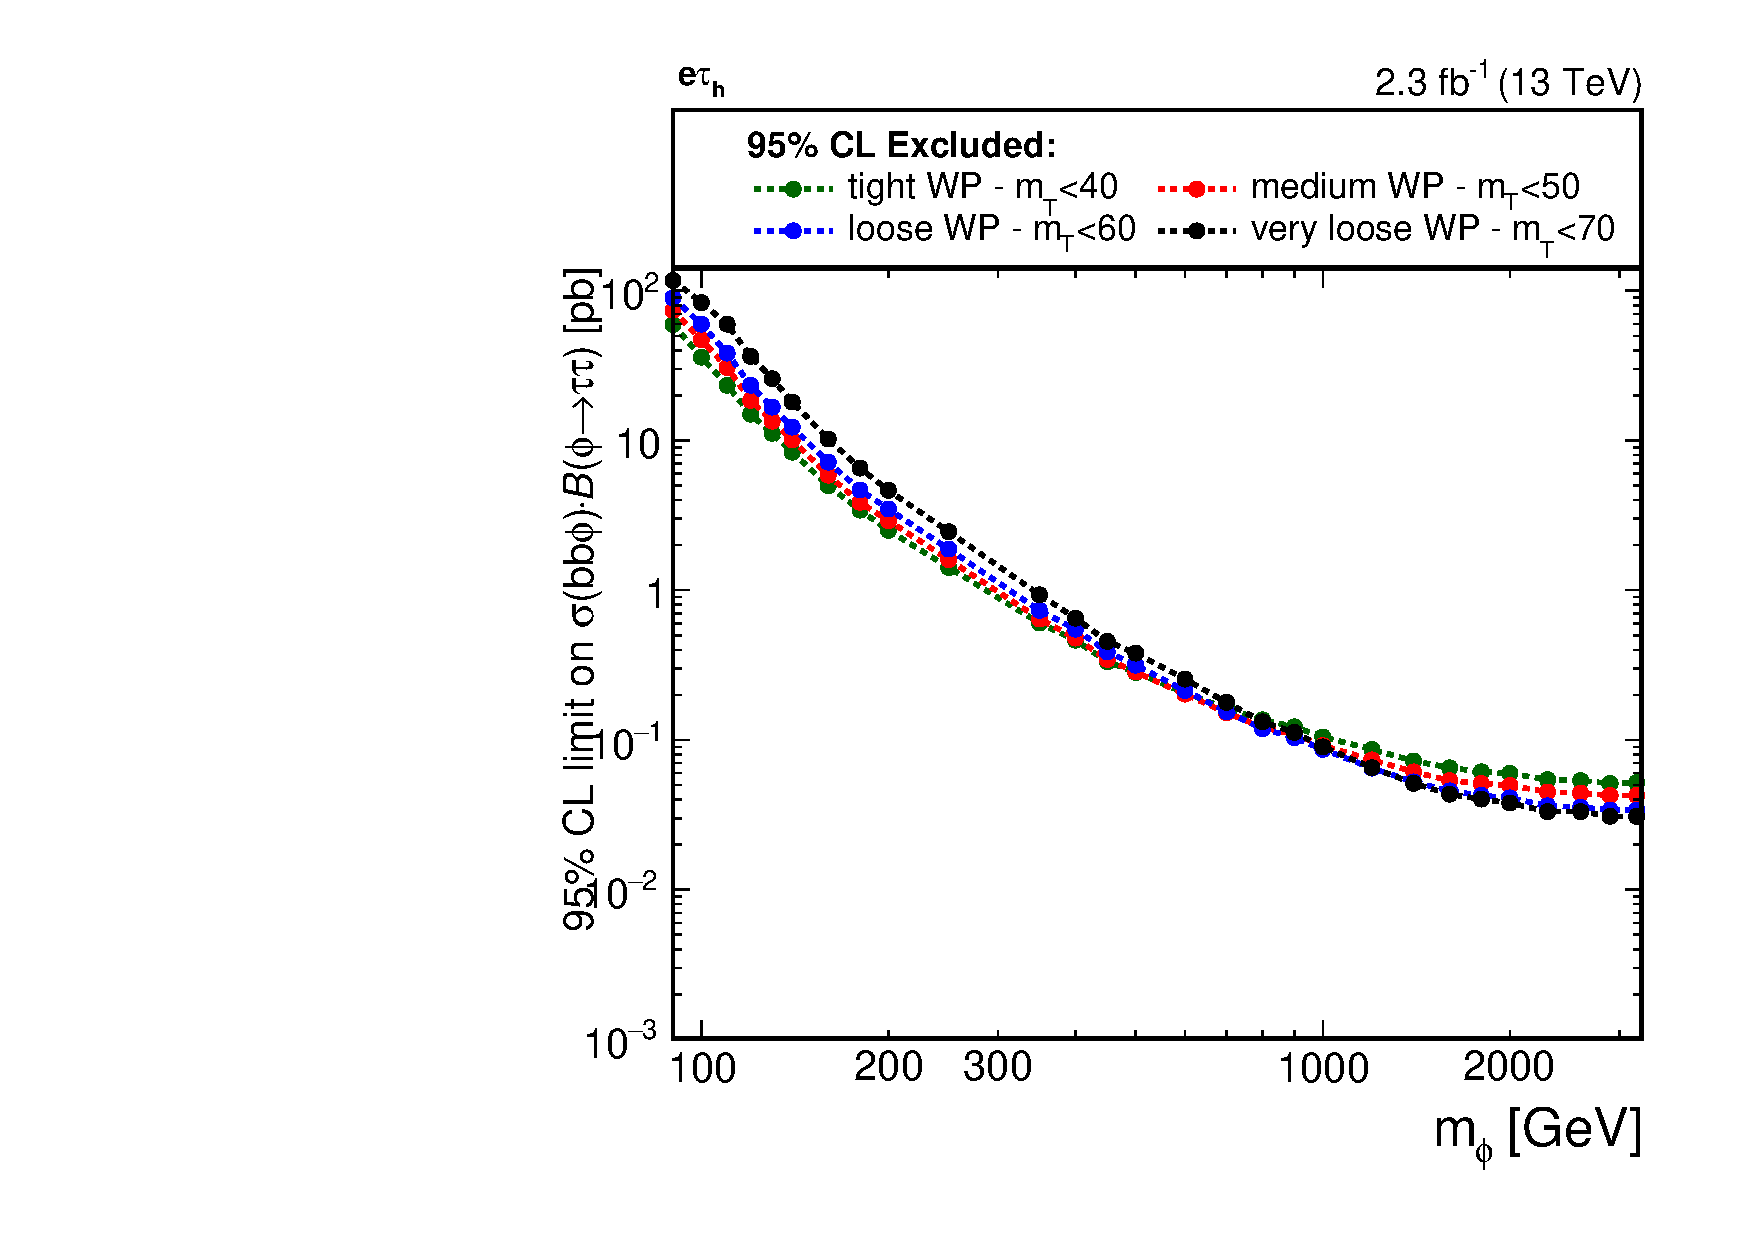
\includegraphics[width=0.5\textwidth]{./MSSM/Figures/mssm_gradcuts_bbH_et.pdf}}
\end{center}
\caption[Pre-fit expected limits on $\sigma\times$ BR in the \etau
channel for gg$\phi$ and bb$\phi$ production for an increasingly
looser \mT~selection and tau isolation working point.]{Pre-fit expected limits on $\sigma \times$ BR in the \etau channel for (a) gg$\phi$ and
(b) bb$\phi$ production, for an increasingly looser \mT~selection and tau isolation working point, starting
at the tight working point and \mT$<40$ GeV in green, the medium working point and \mT$<50$ GeV in red,
the loose working point and \mT$<60$ GeV in blue and the very loose working point and \mT$<70$ GeV in black. Loosening
the tau isolation working point and \mT~selection gradually improves limits at higher mass, and
degrades them at low mass.}
\label{fig:mssm_gradcuts_et}
\end{figure}
\begin{figure}[h!]
\begin{center}
\subfloat[gg$\phi$]{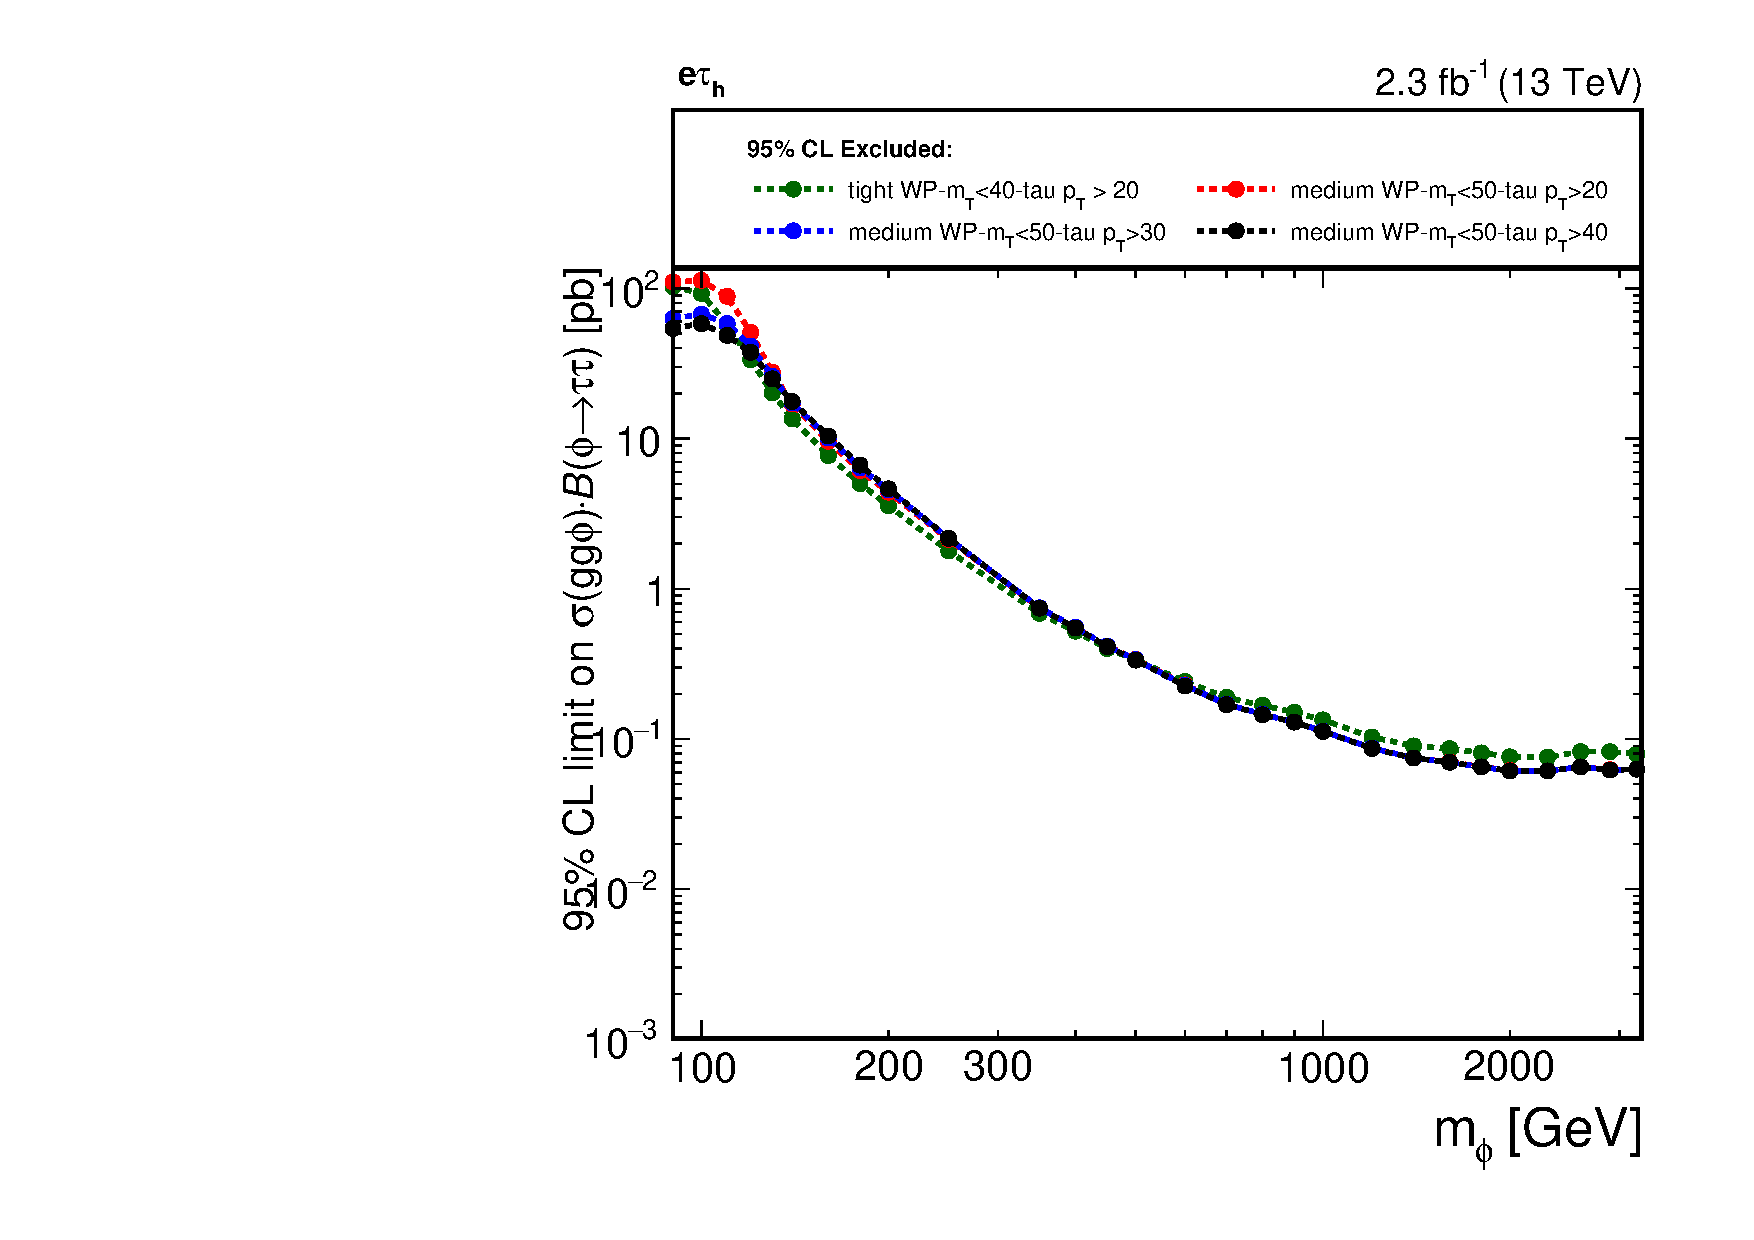
\includegraphics[width=0.5\textwidth]{./MSSM/Figures/mssm_optimisation_mediummt50_vs_tightmt40pt20_et_ggH_remake.pdf}}
\subfloat[bb$\phi$]{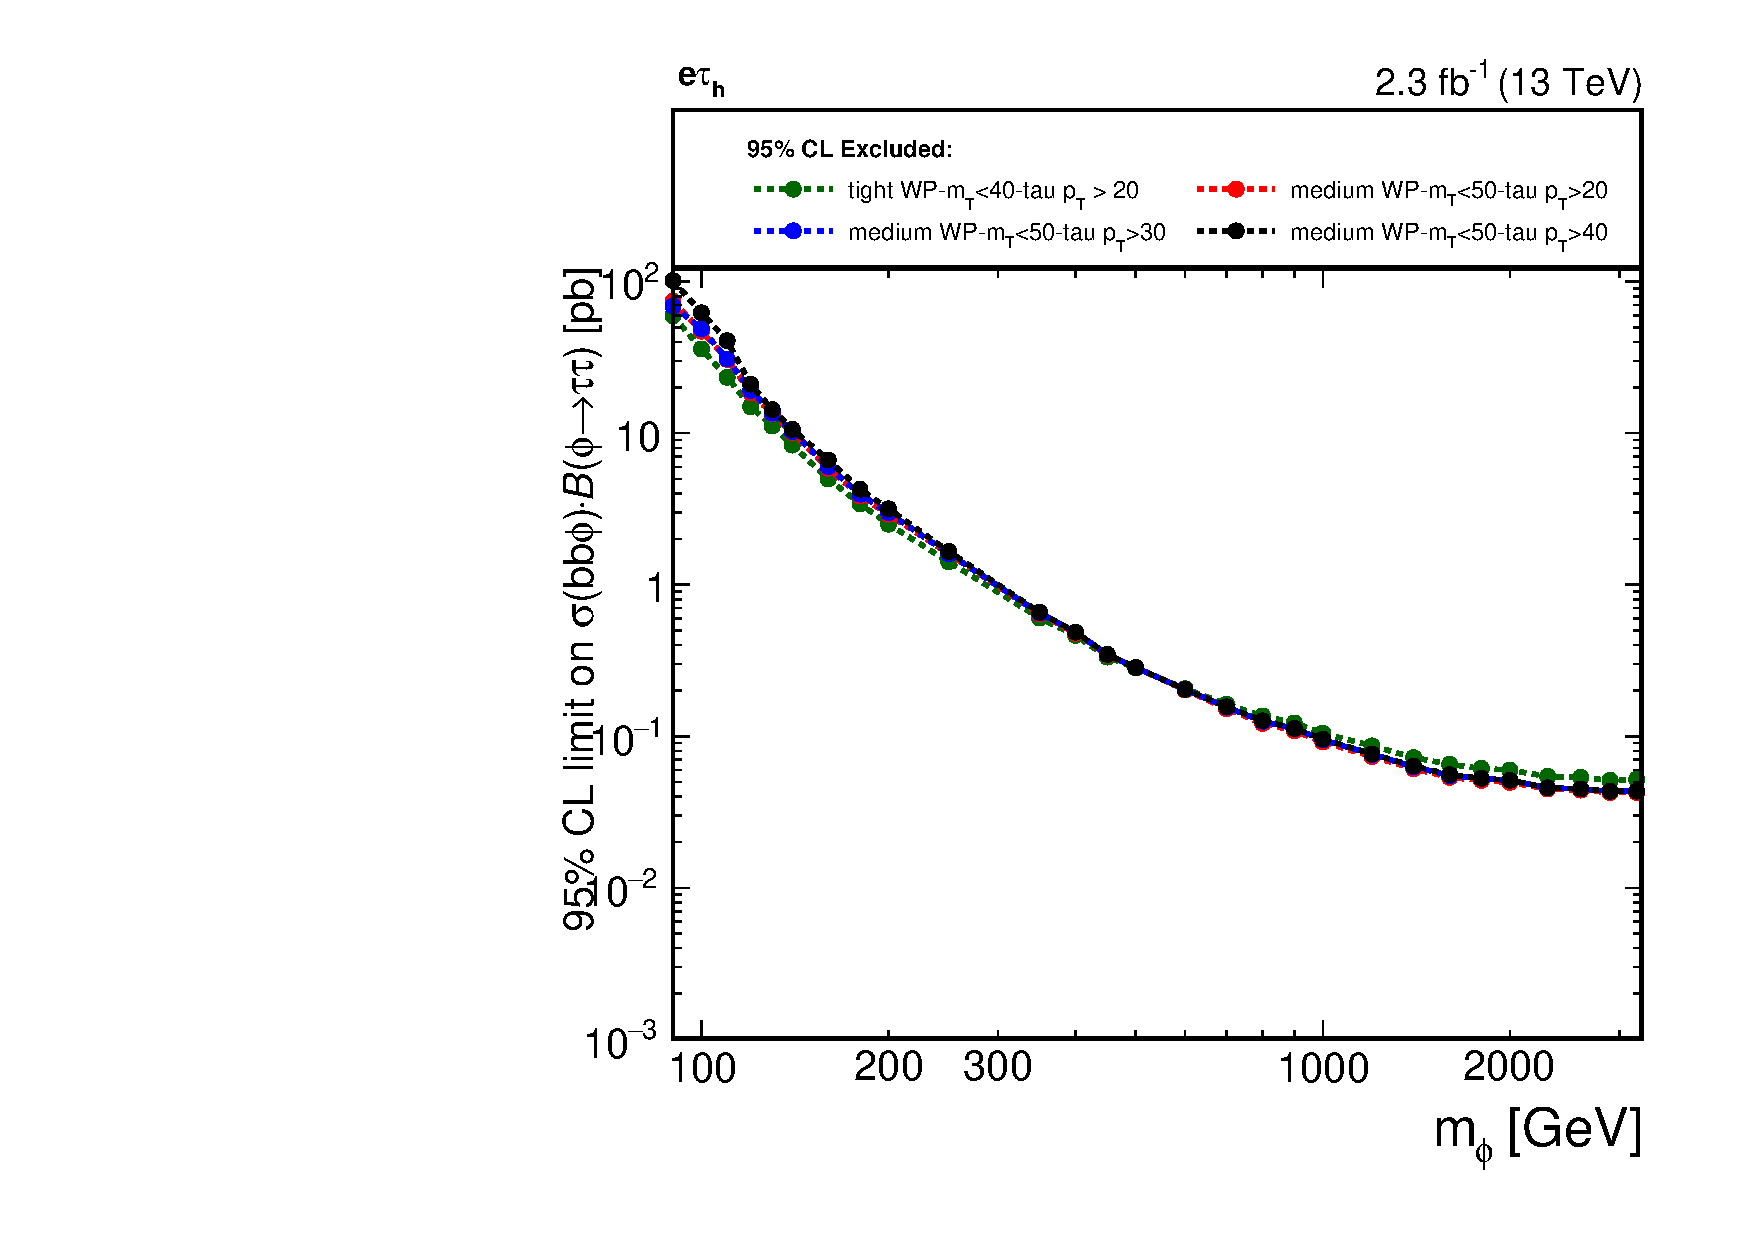
\includegraphics[width=0.5\textwidth]{./MSSM/Figures/mssm_optimisation_mediummt50_vs_tightmt40pt20_et_bbH_remake.pdf}}
\end{center}
\caption[Pre-fit expected limits on $\sigma\times$BR in the \etau
channel for gg$\phi$ and bb$\phi$ production comparing different
hadronic tau isolation cuts.]{Pre-fit expected limits on $\sigma\times$BR in the \etau channel for (a) gg$\phi$ production and (b) bb$\phi$ production. The
limits using the medium hadronic tau isolation working point and \mT$<40$ GeV selection using a minimum
hadronic tau \pT~cut of 20 GeV (red circles), 30 GeV (blue circles) and 40 GeV (black circles) are shown. The green
circles show the limits using tighter tau isolation working point and \mT~selection. The limits on
the gg$\phi$ production process improve at low masses when increasing the hadronic tau \pT~cut,
the effect on the bb$\phi$ production process is less pronounced.}
\label{fig:mssm_tauptcut_et}
\end{figure}

\subsection{\texorpdfstring{Event selection in the \tautau channel}{Event selection in the tau tau channel}}
\label{sec:mssm_eventsel_tt}
The trigger in the \tautau channel requires two hadronic taus at \ac{L1} and the \ac{HLT}
applies loose identification and isolation criteria to these hadronic taus.

The offline event selection requires both hadronic taus to be oppositely charged, separated
by $\Delta R > 0.5$, have \pT~of at least 40 GeV and satisfy $|\eta|<2.1$. Both taus need
to be reconstructed by the HPS algorithm, and their impact parameter $d_{z}$ must be less than 0.2 cm.
Both taus need to pass the tight working point of the isolation discriminator, the very loose 
working point of the anti--electron discriminator and the loose working point of the anti--muon discriminator. 
The tight working point of the isolation discriminator is chosen such that
the channel is near-optimal at high mass, while not losing too much sensitivity in the low-intermediate mass range.
This is illustrated in figure \ref{fig:mssm_tauid_tt} for the gg$\phi$ process.

\begin{figure}[h!]
\begin{center}
\subfloat[gg$\phi$]{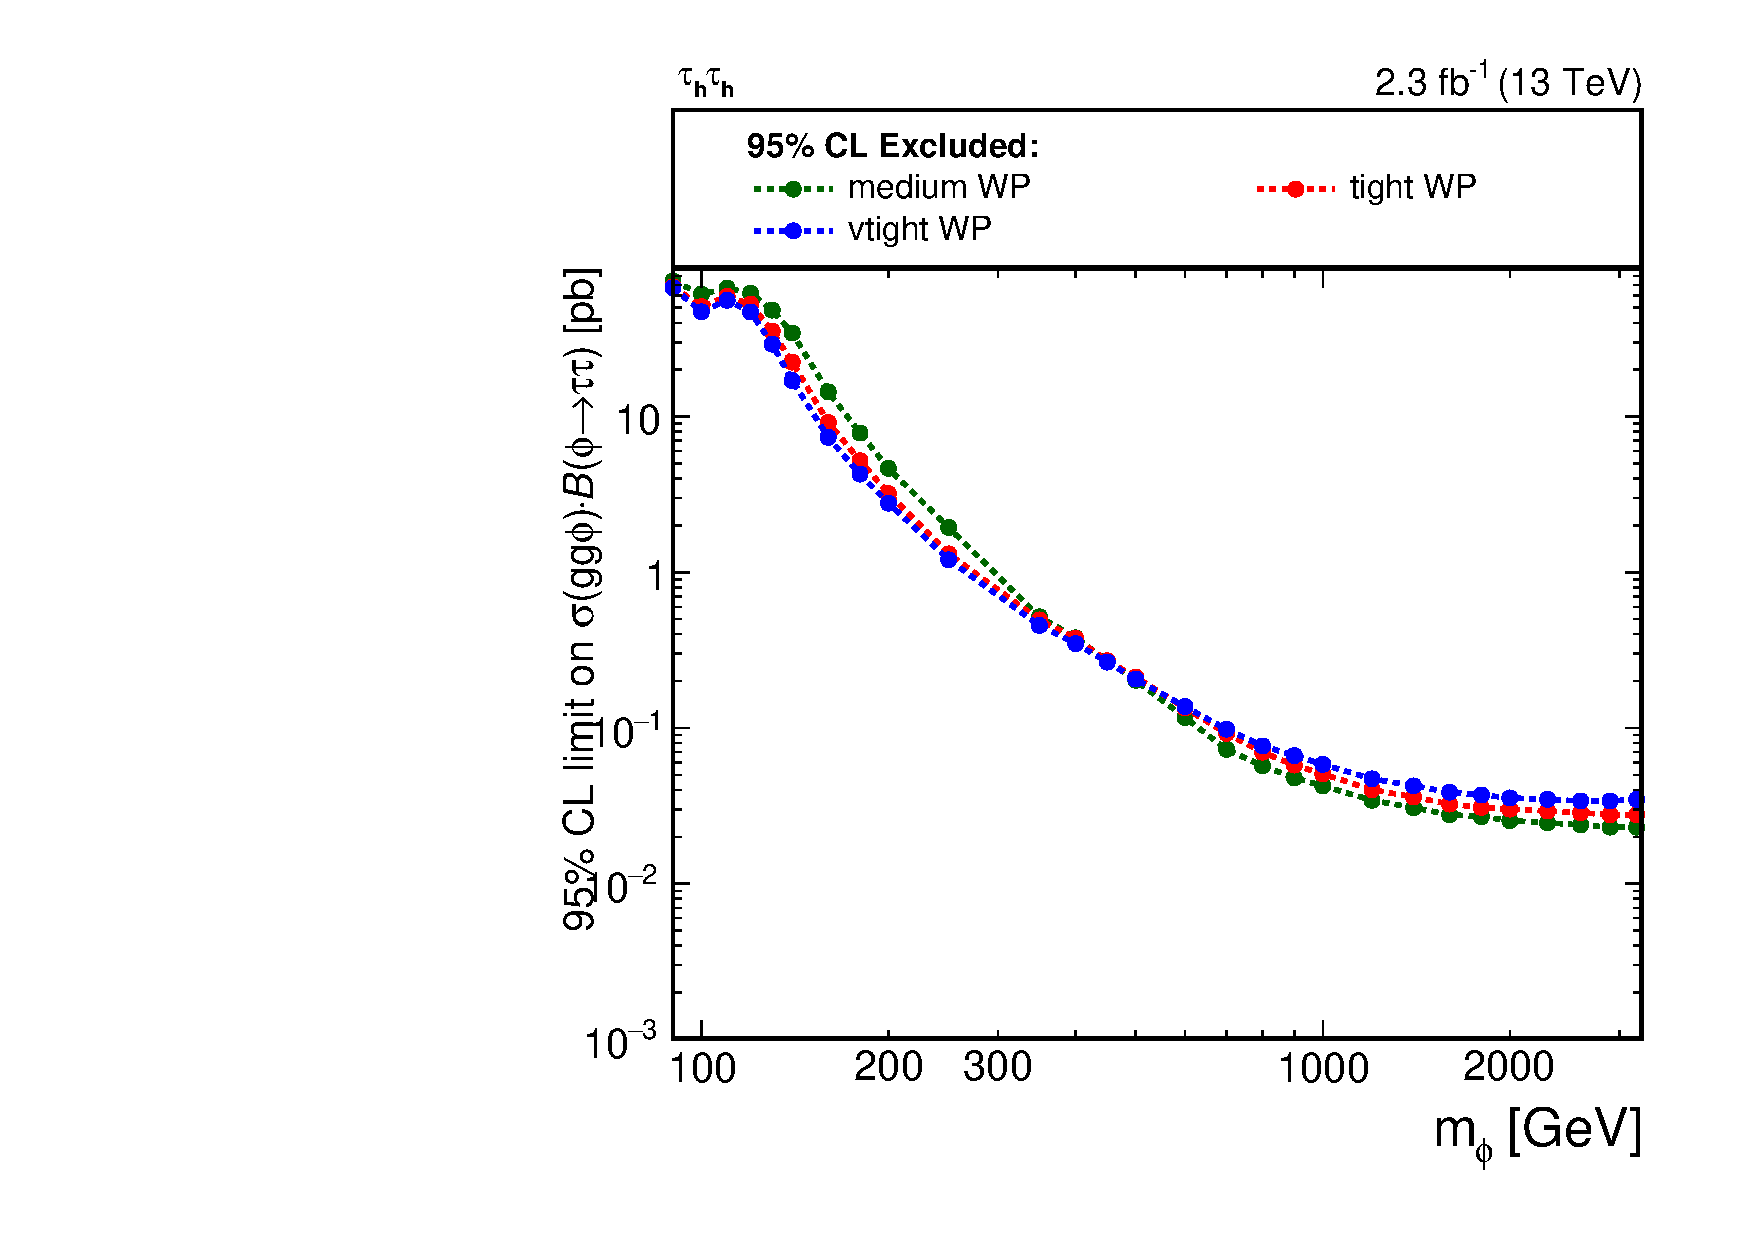
\includegraphics[width=0.5\textwidth]{./MSSM/Figures/mssm_thesis_ttopt_ggH.pdf}}
\subfloat[bb$\phi$]{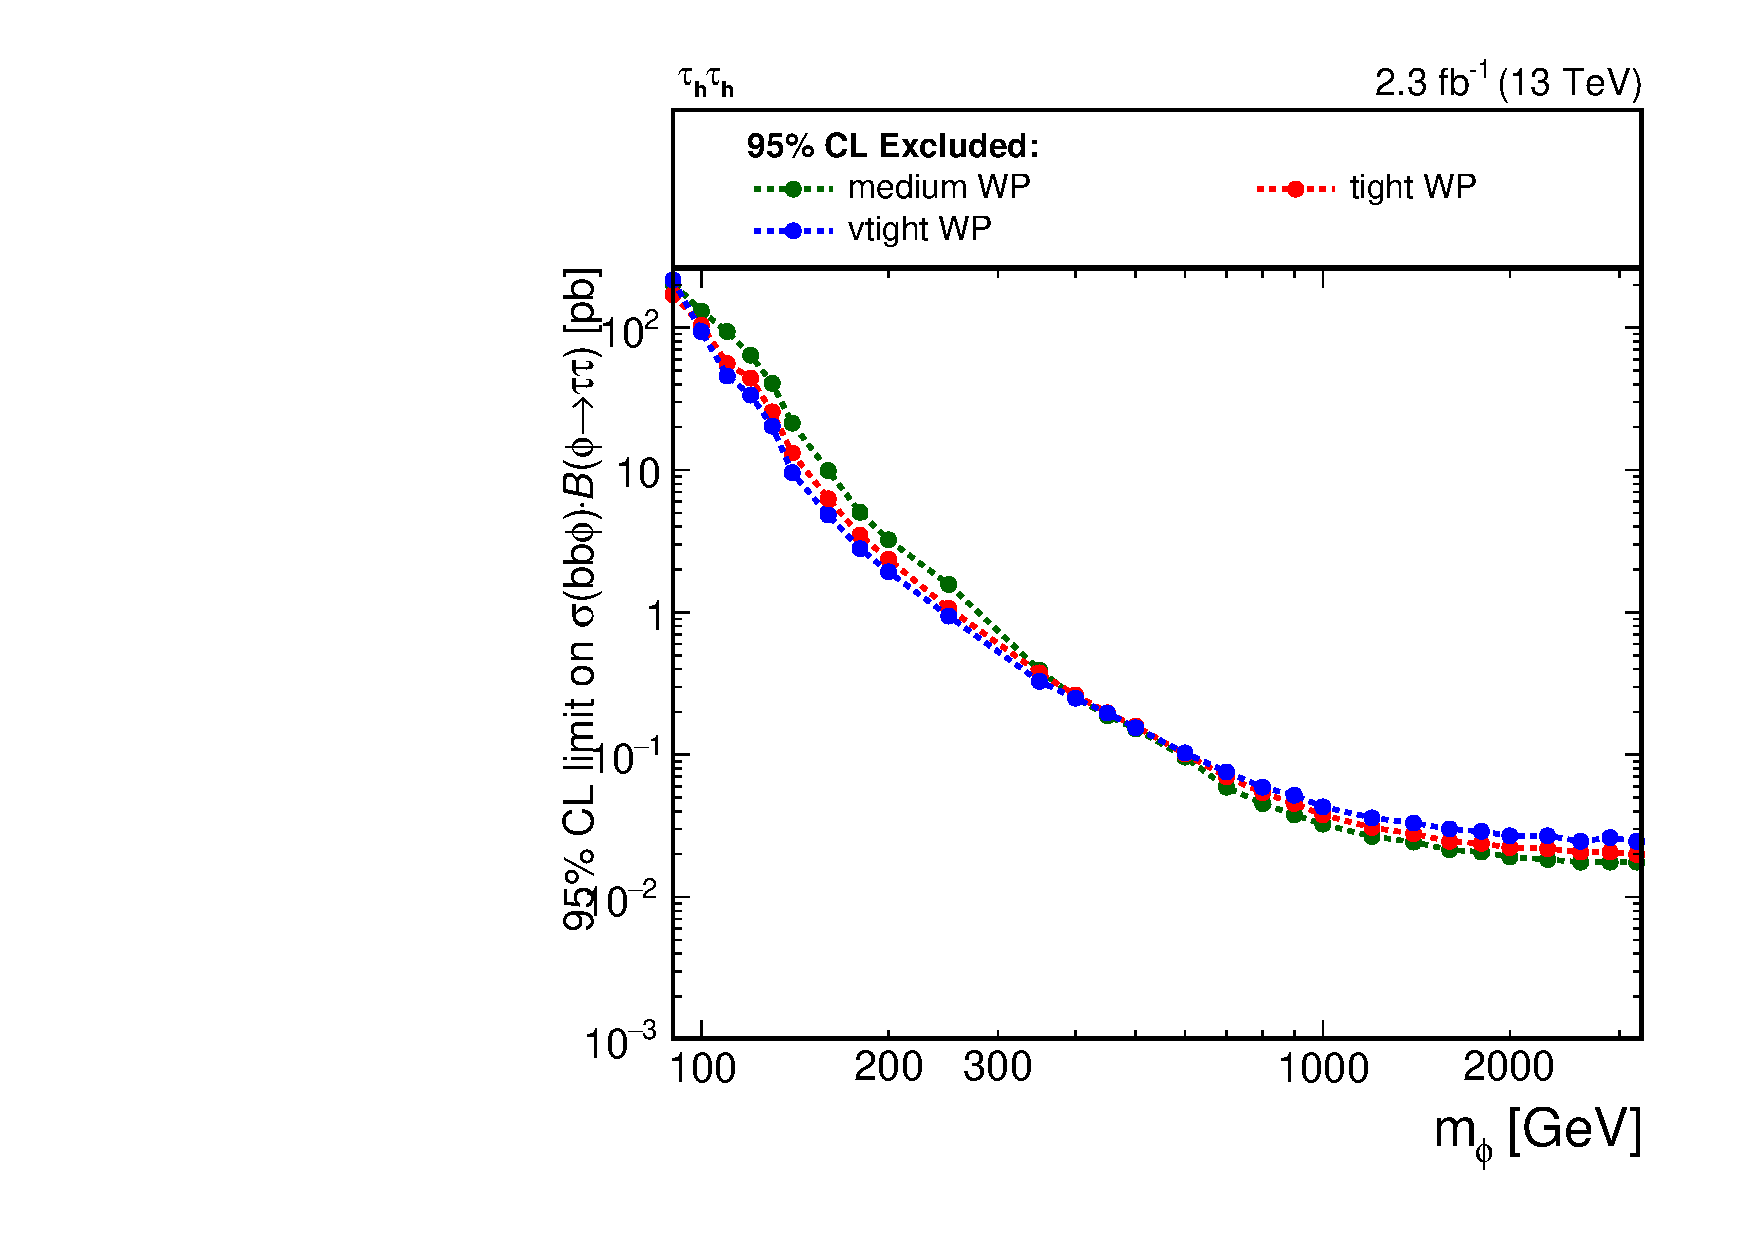
\includegraphics[width=0.5\textwidth]{./MSSM/Figures/mssm_thesis_ttopt_bbH.pdf}}
\end{center}
\caption[Expected upper limits for the gg$\phi$ and bb$\phi$ process
in the \tautau channel, comparing different hadronic tau isolation working
points.]{Expected upper limits for (a) the gg$\phi$ process and (b) the bb$\phi$ process 
in the \tautau channel, using the 
medium (green), tight (red) and very tight working point of the tau isolation discriminator.
The pattern is roughly the same as in the \etau and \mutau channels, with looser selections preferred at high
mass.}
\label{fig:mssm_tauid_tt}
\end{figure}

\subsection{\texorpdfstring{Event selection in the \emu channel}{Event selection in the e mu channel}}
\label{sec:mssm_eventsel_em}
Events in the \emu channel are first selected by two triggers
that both require an electron and muon at \ac{L1} and apply loose ID and
isolation requirements to these objects at \ac{HLT}. The \pT~requirements on
the electron and muon are different in the two triggers, thus using the combination of the two
improves the signal efficiency.

Offline, the electron and muon are required to be oppositely charged
and separated by $\Delta R >$0.3.
The electron needs to have a minimum \pT~of 13 GeV and have $|\eta|< 2.5$. As
in the \etau channel the electron's impact parameters have to 
satisfy $d_{xy} < 0.045$ cm and $d_{z}<0.2$ cm. The additional
identification requirement is identical to the criterium applied to electrons in the \etau channel.
The electron also needs to be isolated, $I_{\text{rel}}^{\Pe}<0.15$, where the relative isolation variable is calculated
with a cone size of 0.3.

The muon needs to have a \pT~of at least 10 GeV, $|\eta|<2.4$ and 
its impact parameters need to be $d_{xy}<0.045$ cm and $d_{z}<0.2$ cm.
In addition to the kinematic requirements the muon must
pass the medium identification criteria and be isolated with $I_{\text{rel}}^{\Pgm} < 0.2$,
where the relative isolation variable is calculated using a cone size of 0.4.

Because a combination of triggers is used, one with electron \pT~$>$ 23 GeV and muon \pT~$>8$ GeV
and one with muon \pT~$>$ 23 GeV and electron \pT~$>$ 13 GeV, the object firing
the higher \pT~trigger leg needs to have a transverse momentum
of at least 24 GeV on top of the requirements already discussed. This avoids
events in the lower part of the trigger turn-on curve being selected.

In addition to the selection described so far,
 a topological selection is made on the $D_{\zeta}$ variable \cite{cdf-dzeta},
\begin{align}\label{eqn:mssm_em_dzeta}
D_{\zeta} = P_{\zeta} - 1.85 P_{\zeta}^{\text{vis}}, \notag \\
\text{where } P_{\zeta} = (\vec{p}_{\text{T},1}^{\text{  vis}} + \vec{p}_{\text{T},2}^{\text{  vis}} + E_{\text{T}}^{\text{miss}})\frac{\vec{\zeta}}{|\vec{\zeta}|}, \notag \\
\text{and } P_{\zeta}^{\text{vis}} = (\vec{p}_{\text{T},1}^{\text{  vis}}+\vec{p}_{\text{T},2}^{\text{  vis}})\frac{\vec{\zeta}}{|\vec{\zeta}|}.
\end{align}
This means $D_{\zeta}$ is defined as the projection of the transverse momenta of the visible tau decay products plus missing energy \pT+\MET~onto 
the axis $\vec{\zeta}$, minus the projection of only the transverse momenta of the visible tau decay products onto this axis.
The axis $\vec{\zeta}$ is the axis that bisects
the directions $\vec{p}_{\text{T,1}}^{\text{  vis}}$ and $\vec{p}_{\text{T,2}}^{\text{  vis}}$
of the visible decay products in the transverse plane. This definition is illustrated in figure
\ref{fig:mssm_dzeta}a, with figure \ref{fig:mssm_dzeta}b showing the $D_{\zeta}$ distribution
for \emu events. The selection used, $D_{\zeta} > -20$ GeV, rejects $\ttbar$, \Wjets and diboson
events. 
%The momentum of the neutrinos should not be in the opposite direction of the sum of the visible decay products
%as the neutrinos and visible tau decay products travel at small angles from the original tau.

\begin{figure}[h!]
\begin{center}
\subfloat[Reconstruction of $D_{\zeta}$]{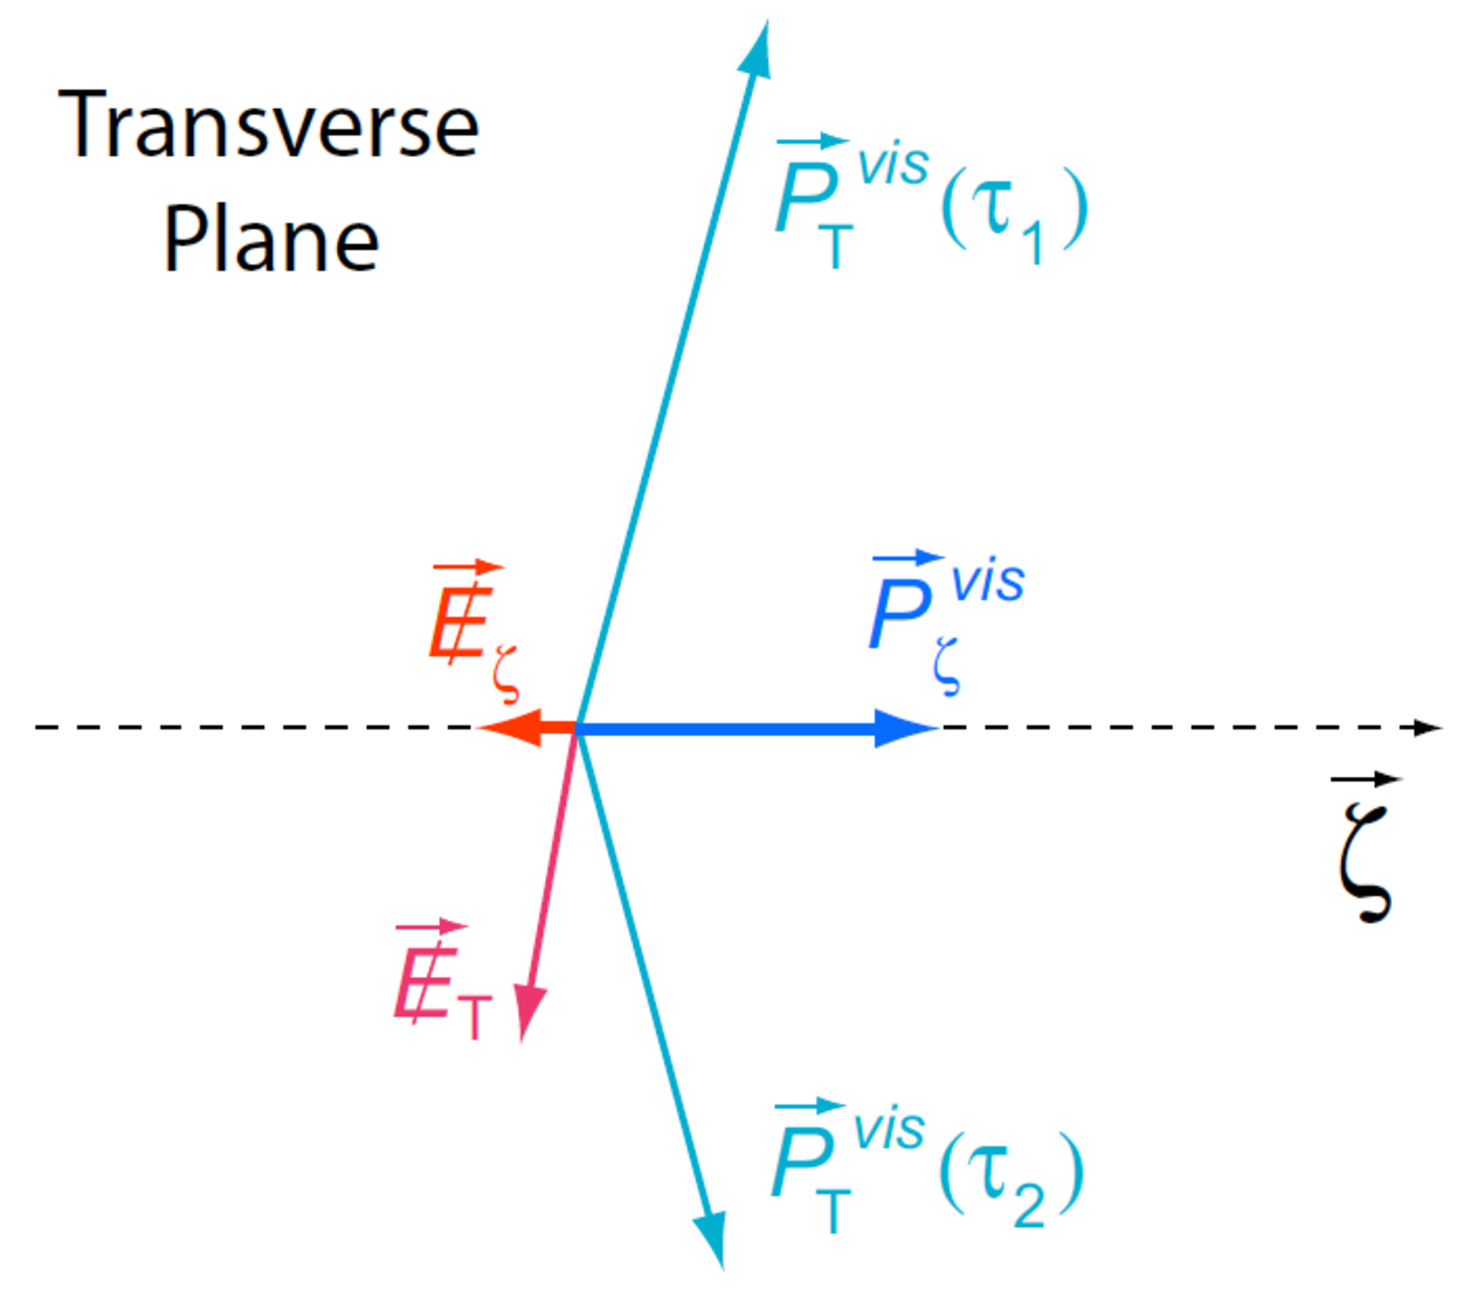
\includegraphics[width=0.5\textwidth]{./MSSM/Figures/PZeta.pdf}}
\subfloat[$D_{\zeta}$ distribution in \emu channel]{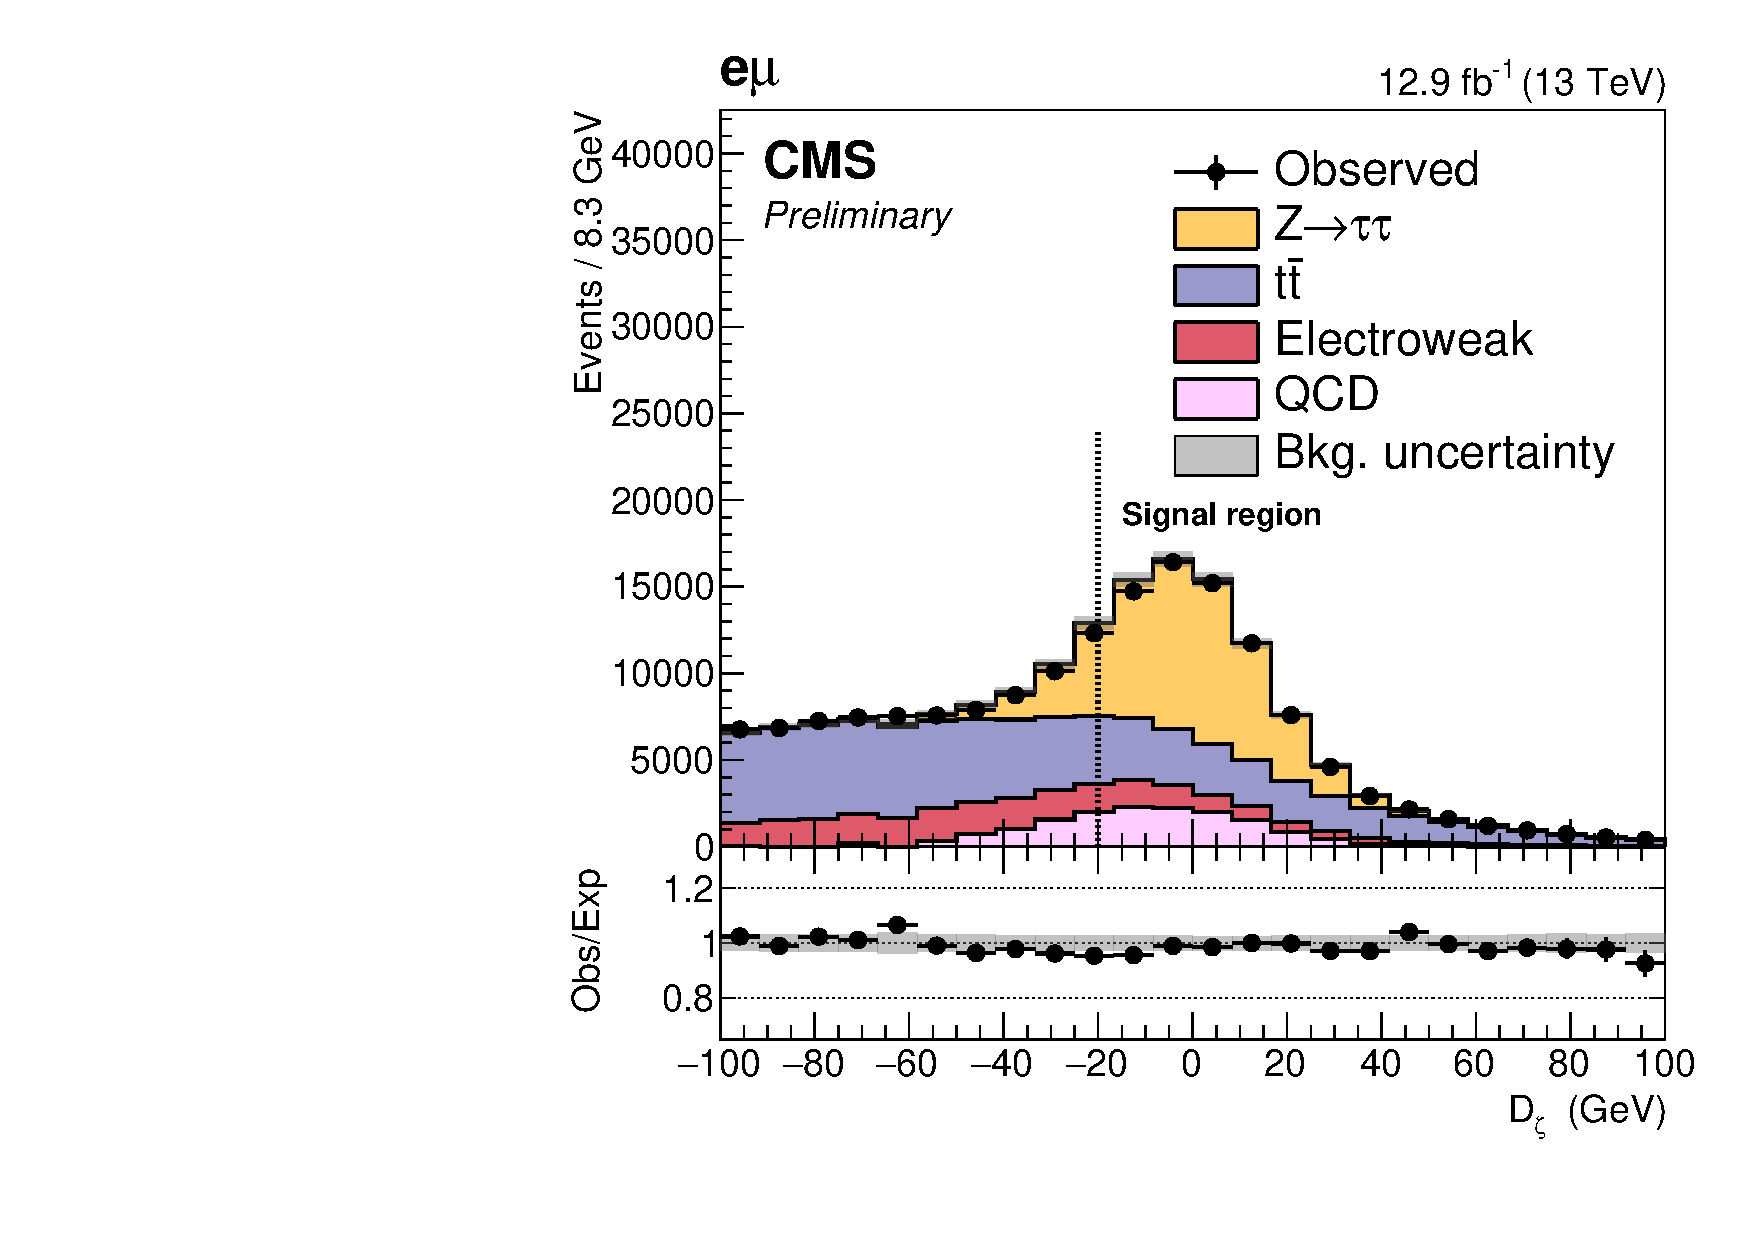
\includegraphics[width=0.5\textwidth]{./MSSM/Figures/pzeta_inclusive_em_2016.pdf}}
\end{center}
\caption[Reconstruction of the $D_{\zeta}$ variable and the $D_{\zeta}$ distribution
in the \emu channel.]{(a) reconstruction of $D_{\zeta}$ \cite{cdf-dzeta} and (b) $D_{\zeta}$ distribution in the 
\emu channel\cite{CMS-PAS-HIG-16-037}.}
\label{fig:mssm_dzeta}
\end{figure}
~\clearpage
\subsection{Categorisation}
\label{sec:mssm_eventsel_categories}
As the analysis targets both the gluon fusion
and the b--associated production modes, 
the sensitivity to the signal can be increased by categorising
based on the number of b--tagged jets in the event.

\begin{figure}[h!]
\begin{center}
\subfloat[Number of jets]{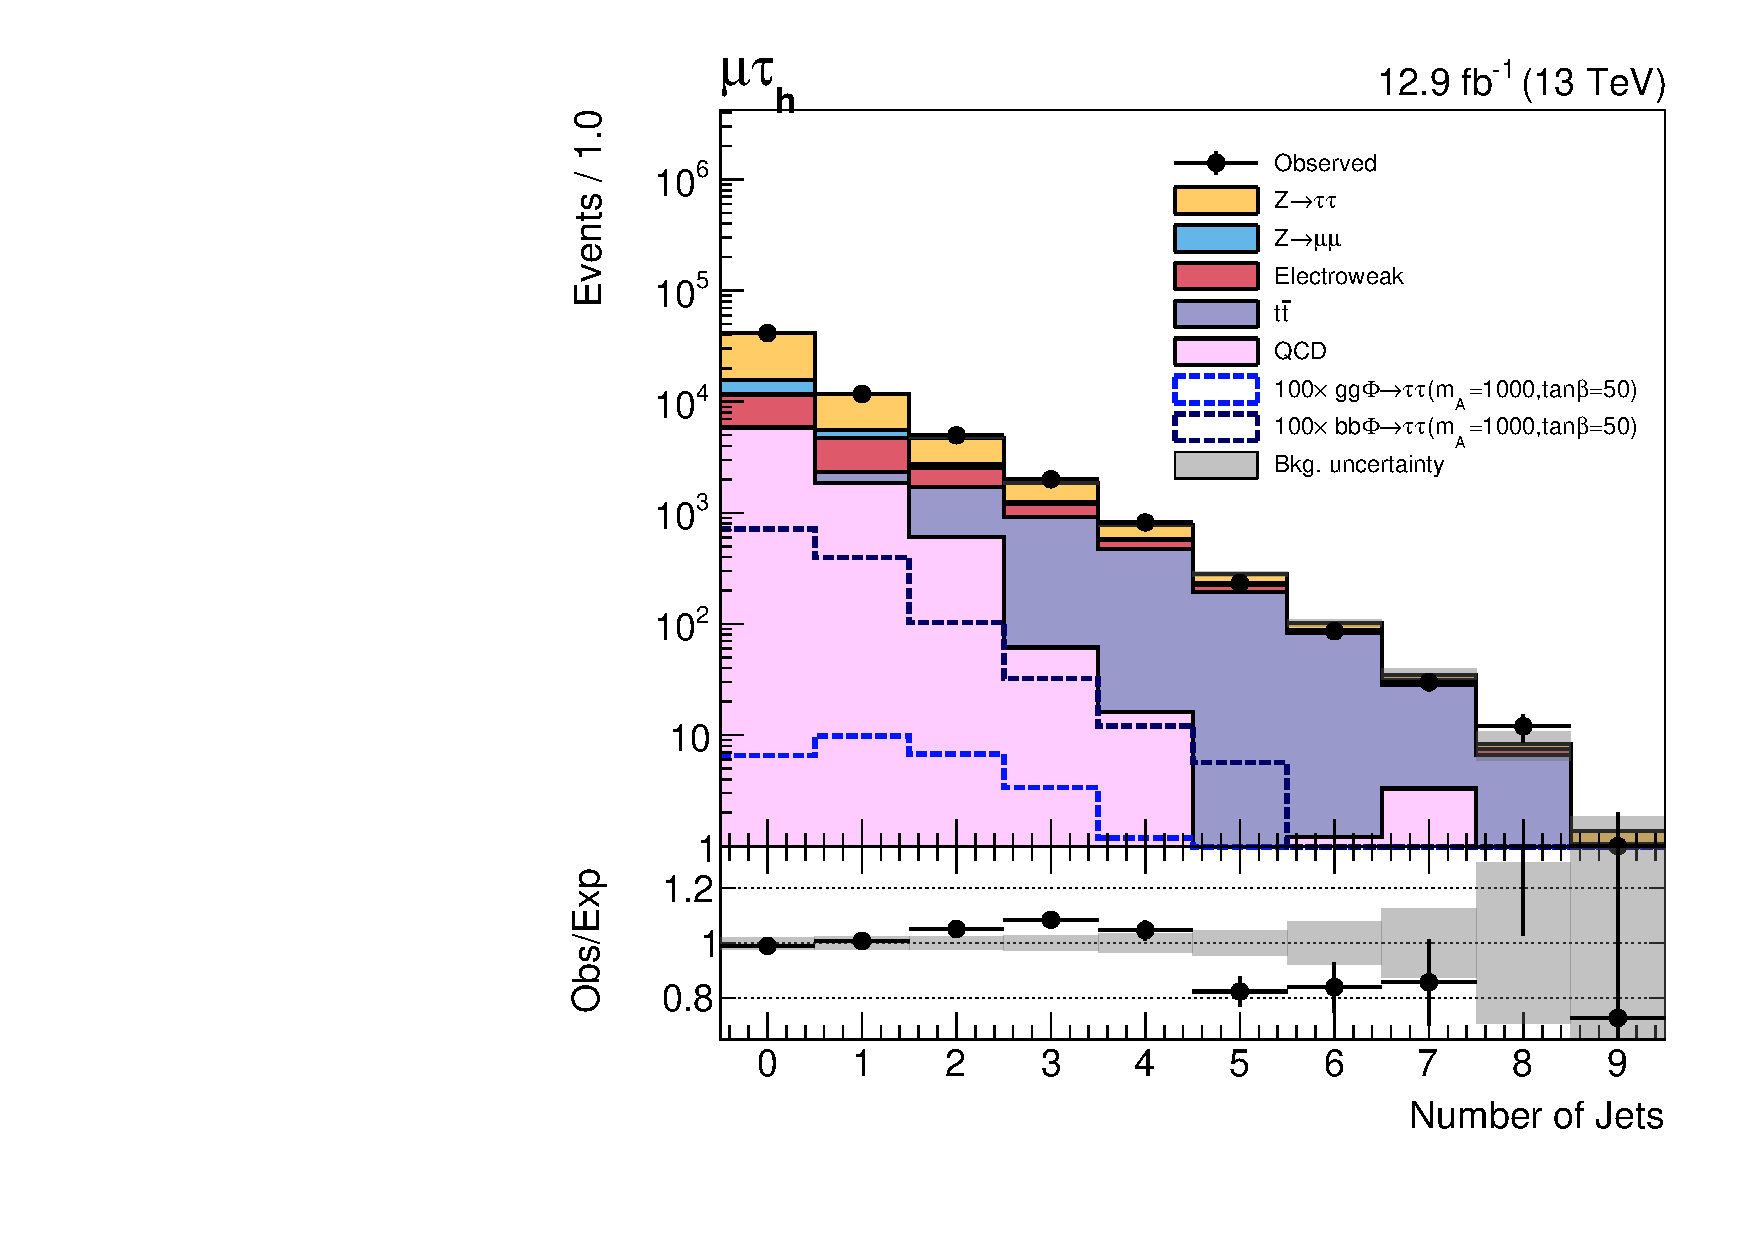
\includegraphics[width=0.5\textwidth]{./MSSM/Figures/n_jets_inclusive_mt_2016_log.pdf}}
\subfloat[Number of b--tagged jets]{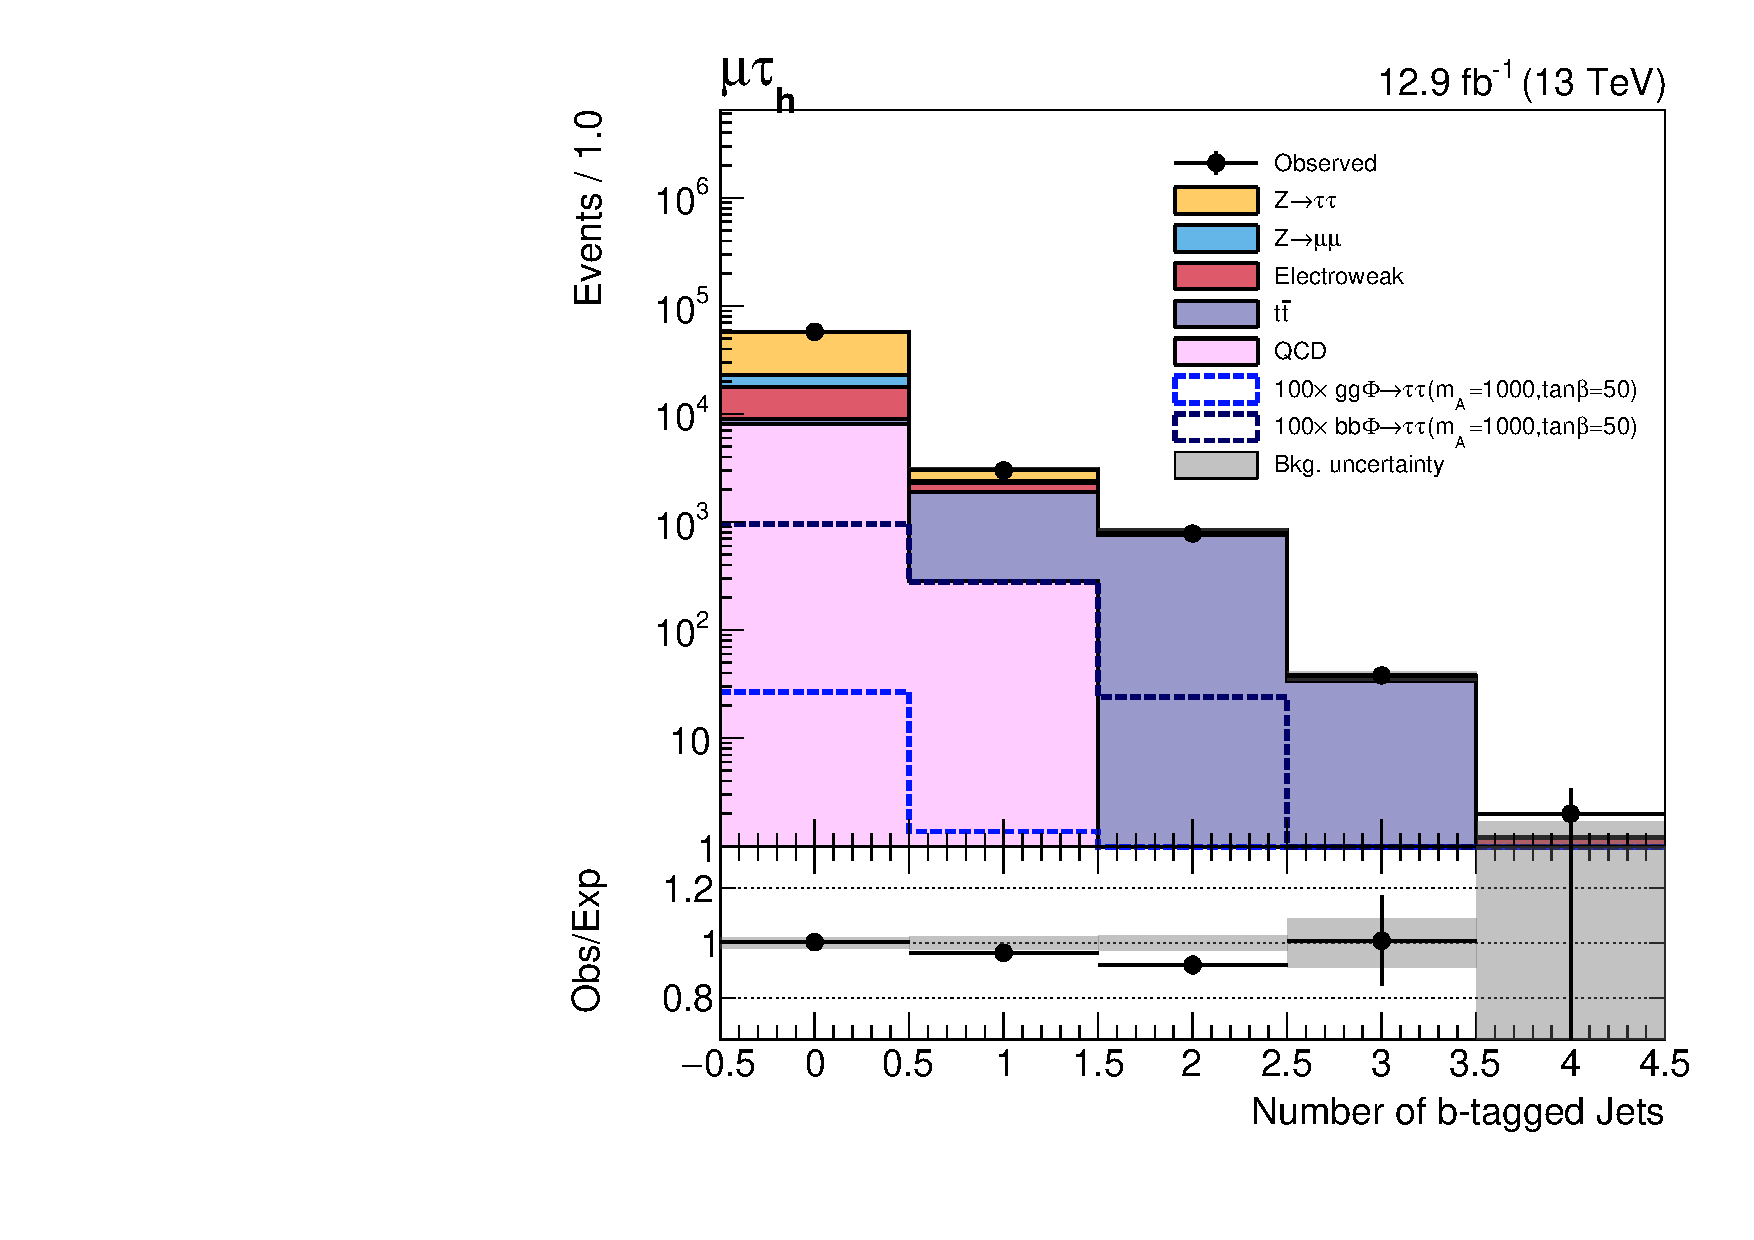
\includegraphics[width=0.5\textwidth]{./MSSM/Figures/n_bjets_inclusive_mt_2016_log.pdf}}
\end{center}
\caption[Number of jets and number of b-tagged jets in the \mutau channel, 
with the signal overlaid.]{(a) Number of jets and (b) number of b--tagged jets in the \mutau channel. The gluon fusion signal (dashed
blue line) and b--associated signal (dashed purple line) are overlaid on the expected background distribution. The signals
are normalised to 100 times their cross--section times branching ratio at \mA=1 TeV and \tanb=50 in the $m_{\text{h}}^{\text{mod+}}$
scenario. We can see how the signal--sensitive bins motivate the choice of categories.}
\label{fig:mssm_cats_mt}
\end{figure}

Figure \ref{fig:mssm_cats_mt}a shows the number of jets 
in the \mutau channel, with figure \ref{fig:mssm_cats_mt}b showing
the number of b--tagged jets in that channel. The gluon fusion
and b--associated signals are overlaid on these distributions, normalised
to 100 times their cross--section times branching ratio at \mA=1 TeV and 
\tanb=50 in the $m_{\text{h}}^{\text{mod+}}$ scenario. From the distribution of the
gluon fusion signal in figure \ref{fig:mssm_cats_mt}b we can 
see that the vast majority of these signal events do not have any b-tagged jets. To
target this production mode we can use a category which requires 0 b-tagged jets.
From the b--associated signal in the same figure we also see that the majority of bb$\phi$
signal events do not have any b-tagged jets either: either the b-jets in these events 
are too soft, or they do not pass the b-tagging requirements. This means that the category
which requires 0 b-tagged jets
is also sensitive to some of the bb$\phi$ signal. To target
the bb$\phi$ signal, we then define another category with at least one b-tagged jet. 
From the bb$\phi$ signal in figure \ref{fig:mssm_cats_mt}b we can also see that there is not
such a large proportion of events with more than 1 b-tagged jet. From figure \ref{fig:mssm_cats_mt}a
we see that the \ttbar background starts to become more sizeable for events with more than
one jet. The definition of the category that targets the bb$\phi$ signal is therefore chosen with the inclusion
of the jet veto, such that the region where the \ttbar background becomes larger is excluded, 
while retaining a large proportion of the bb$\phi$ signal.

In summary, the two categories are defined as:
\begin{itemize}
\setlength{\itemsep}{-\baselineskip}
\item \textbf{No b-tag}: 0 b--tagged jets. This category targets the gg$\phi$ production mode but is also sensitive to some of the bb$\phi$ signal.
\item \textbf{B-tag}: At least 1 b--tagged jet, at most 1 
jet with \pT$>30$ GeV. This second requirement, the jet veto, reduces the \ttbar background. 
Due to the different phase space considered for
b--tagging than for default jet reconstruction this requirement does not necessarily
mean there will be only one b--tagged jet in the event.
\end{itemize}

\section{Discriminating variable}
\label{sec:mssm_discrvar}
The discriminating variable used for signal extraction is the total transverse mass,
\begin{equation}\label{eqn:mttot}
m_{\text{T}}^{\text{tot}} = \sqrt{(m_{\text{T}}(E_{\text{T}}^{\text{miss}},\tau_1^{\text{vis}}))^2+
(m_{\text{T}}(E_{\text{T}}^{\text{miss}},\tau_2^{\text{vis}}))^2 + (m_{\text{T}}(\Pgt_1^{\text{vis}},\Pgt_2^{\text{vis}}))^2}.
\end{equation}

$m_{\text{T}}(1,2)$ is defined as,
\begin{equation}\label{eqn:mttot_12}
m_{\text{T}}(1,2) = \sqrt{2p_{\text{T},1}p_{\text{T},2}(1-\cos{(\Delta\phi(1,2))})}.
\end{equation}

This means that $m_{\text{T}}(E_{\text{T}}^{\text{miss}},\Pgt_1^{\text{vis}})$ is equivalent
to the \mT~defined for the \etau and \mutau channels in equation \ref{eqn:hhh_selection_mt}.
The \mTtot~variable provides good separation between signal and QCD multi--jet events
in the \etau, \mutau and \tautau channels, and between
signal and \ttbar events in the \emu channel. These are some of the 
major backgrounds and thus good separation between these processes and 
the signal is important for the sensitivity of the analysis.
The separation between signal and backgrounds is illustrated in figure
\ref{fig:mttot_sigseps}, where figure \ref{fig:mttot_sigseps}a shows the total transverse mass
distribution of the QCD
background in the no b-tag category of the \tautau channel with the gluon fusion
signal at 400 GeV, 1 TeV and 2 TeV overlaid. Figure \ref{fig:mttot_sigseps}b
shows the total transverse mass distribution of the \ttbar background in the b-tag category of the \emu channel with
the b-associated production signal at the same three masses overlaid. 

\begin{figure}[h!]
\begin{center}
\subfloat[QCD and signal in \tautau no b-tag]{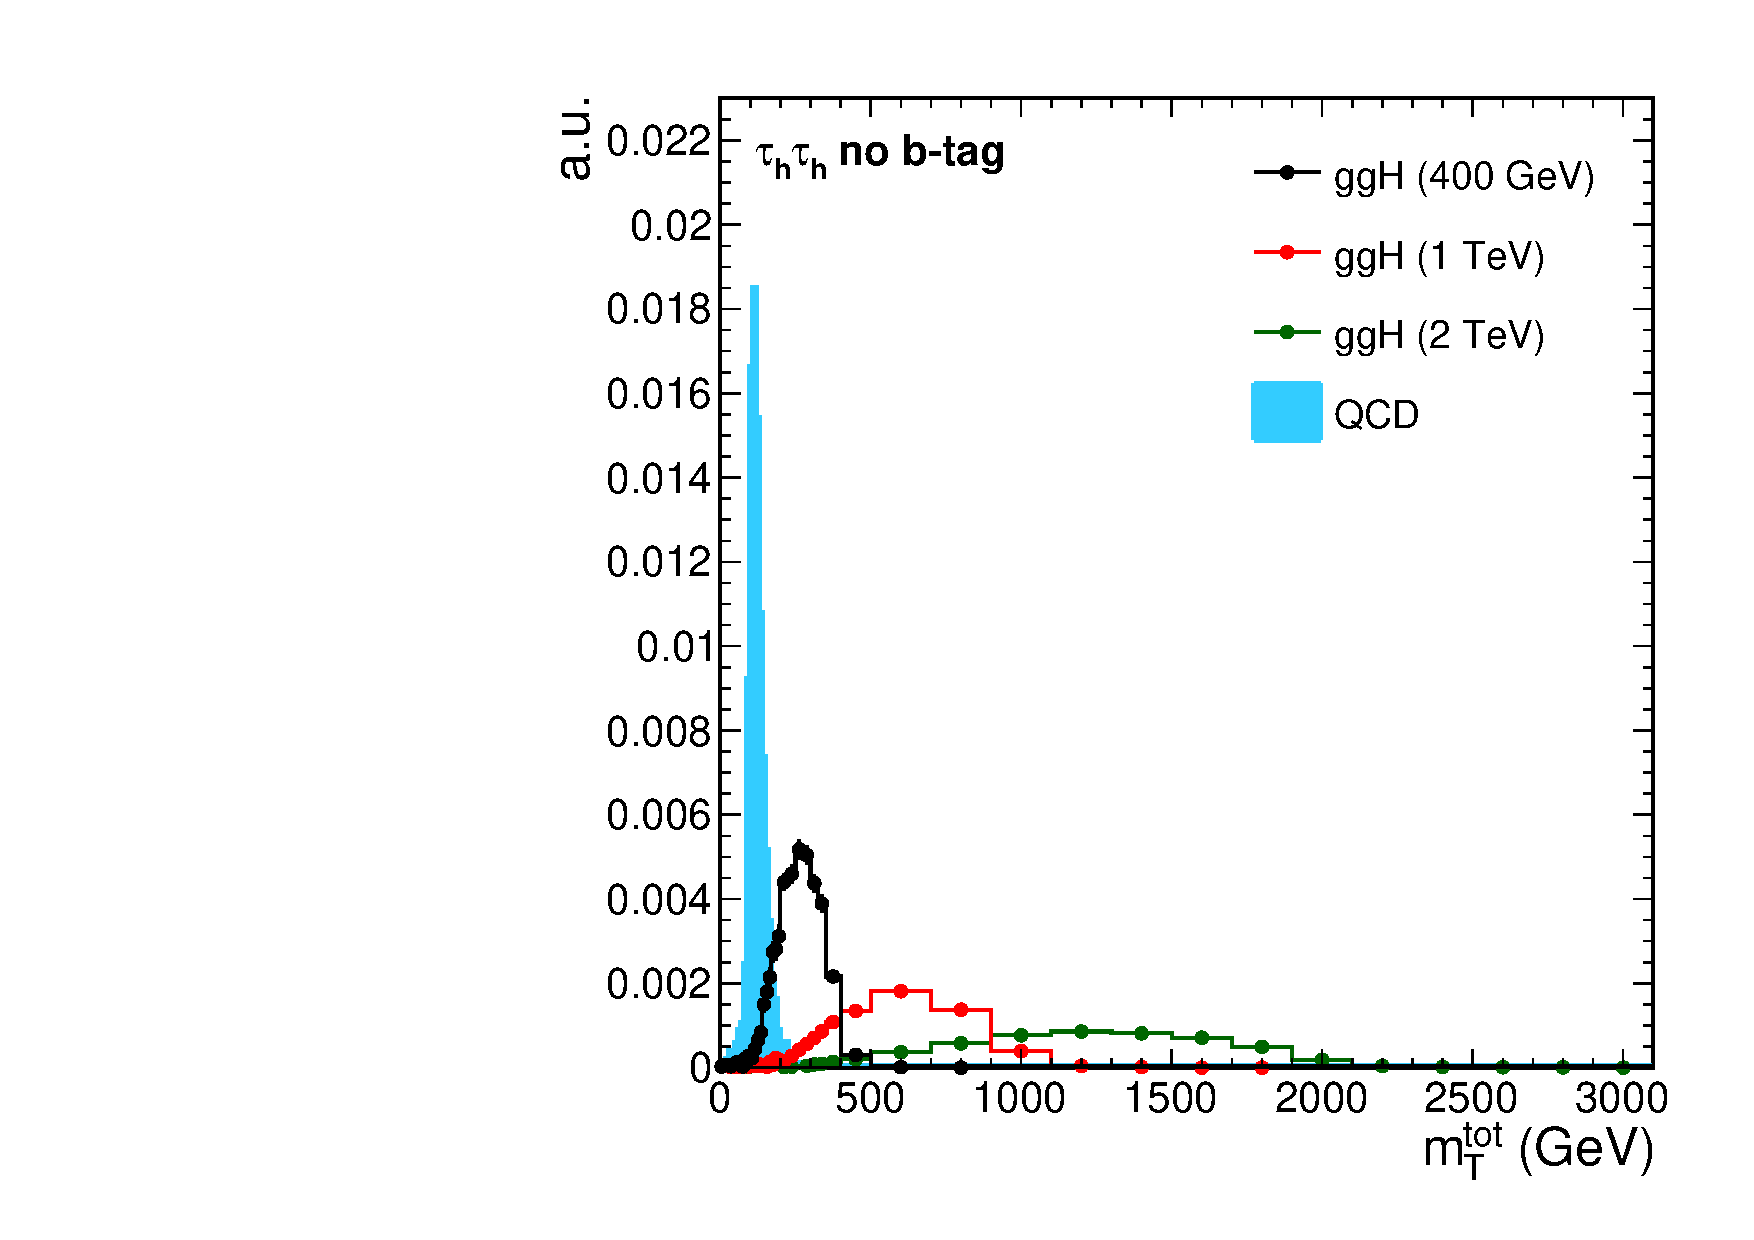
\includegraphics[width=0.5\textwidth]{./MSSM/Figures/mttot_sigsep_tt_nobtag.pdf}}
\subfloat[\ttbar and signal in \emu b-tag]{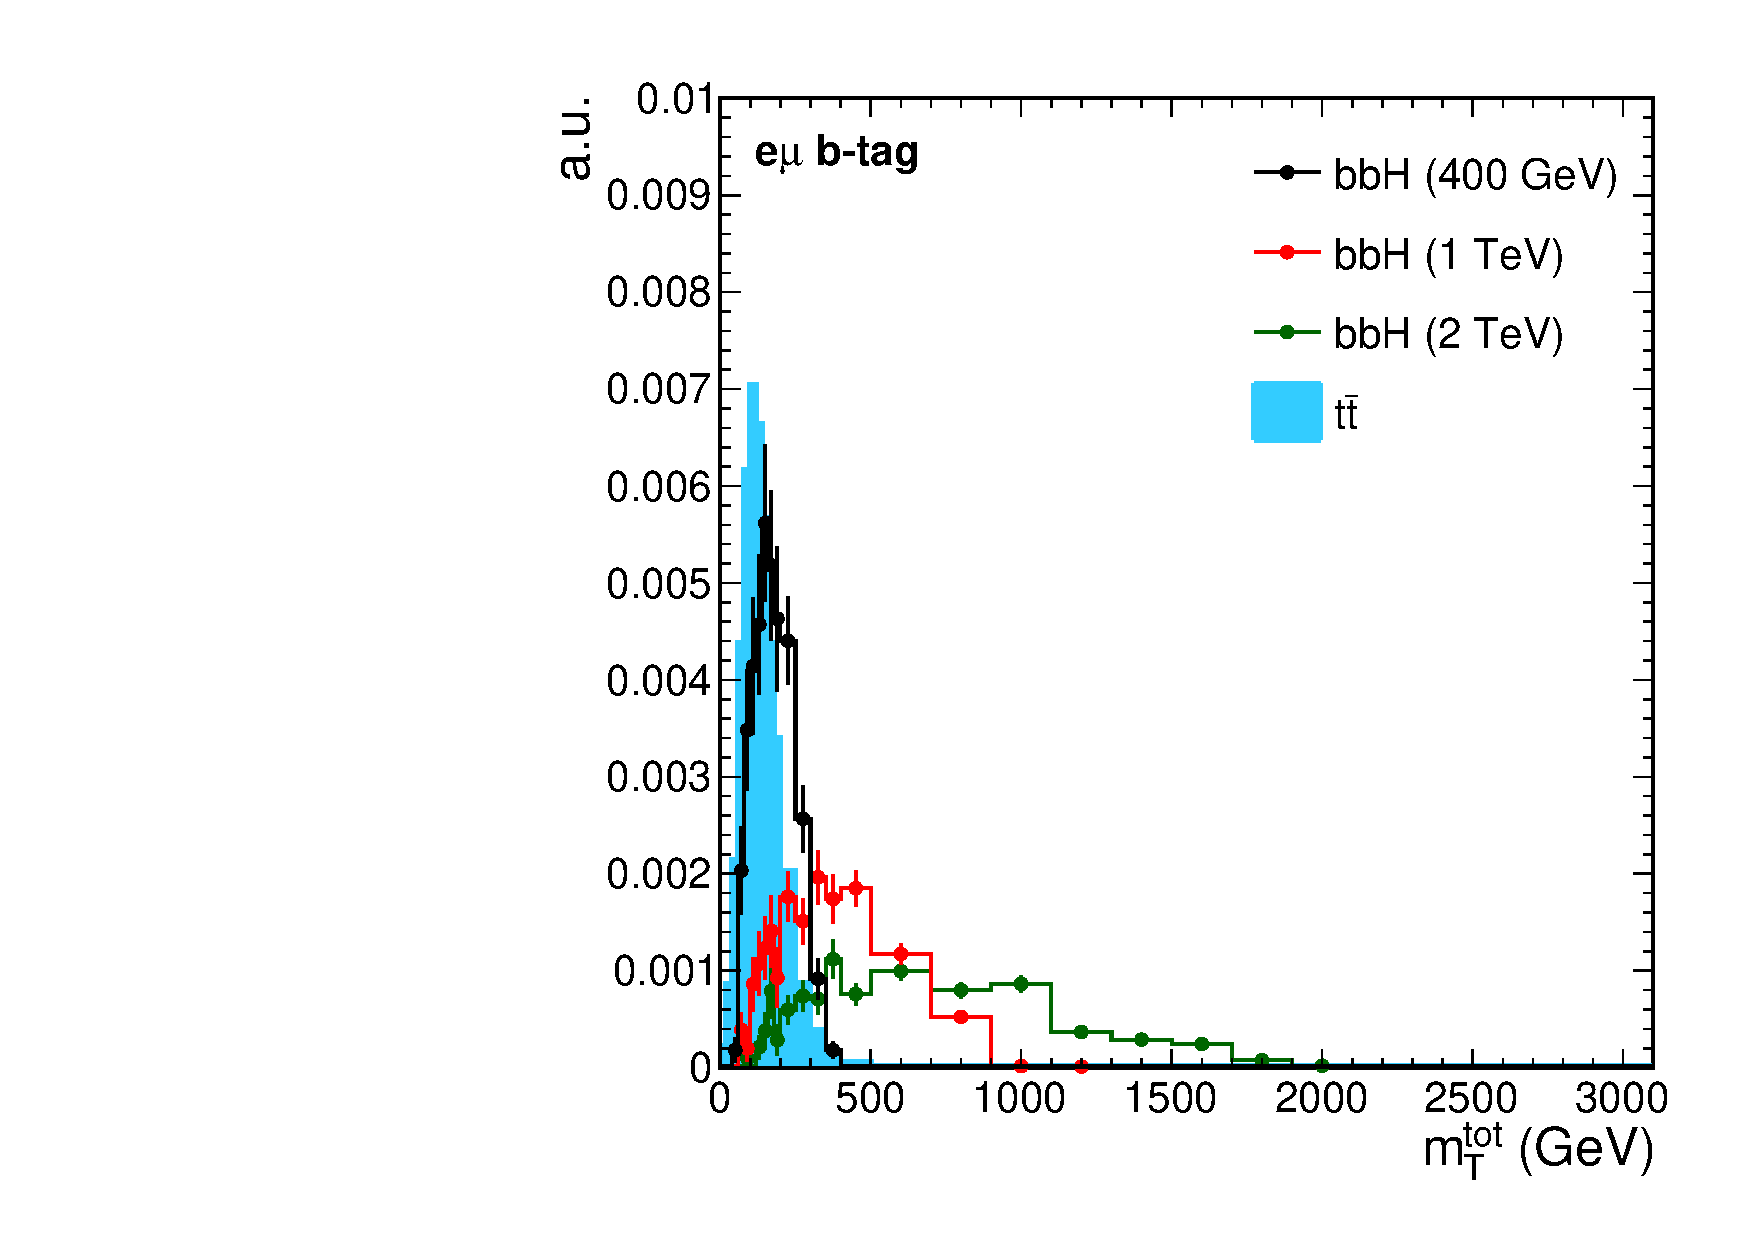
\includegraphics[width=0.5\textwidth]{./MSSM/Figures/mttot_sigsep_em_btag.pdf}}
\end{center}
\caption[Total transverse mass distributions in the no b-tag category of the
\tautau channel for QCD and gluon fusion signal, and in the b-tag category
of the \emu channel, for \ttbar and b-associated signal.]{Total transverse mass distributions in (a) the no b-tag category of the \tautau
channel, for QCD and gluon fusion signal at 400 GeV and 1 and 2 TeV overlaid and (b) in the b-tag
category of the \emu channel, for \ttbar and b-associated signal at 400 GeV and 1 and 2 TeV. 
The total transverse mass variable separates the signal and these backgrounds well.}
\label{fig:mttot_sigseps}
\end{figure}



\section{\acs{MC} to data correction factors}
\label{sec:mssm_mccorrs}
Because \ac{MC} samples are used for the signal prediction, and 
to estimate some of the backgrounds, it is important to correct for possible 
mis-modelling with respect to the data. Dedicated control regions in
data are used to derive the \ac{MC} to data correction factors
that are applied to the \ac{MC} samples. Where efficiencies
are involved this scale factor is derived by measuring the efficiency
in data and in \ac{MC} and constructing the scale factor as $\text{SF}=\frac{\epsilon_{\text{Data}}}{\epsilon_{\text{MC}}}$.
\subsubsection*{Tracking efficiency}
A discrepancy between the track reconstruction efficiency
in data and \ac{MC} for electrons and muons was found. It is corrected for using $\eta$--dependent
scale factors.% \cite{CMS-PAS-HIG-16-037}.
\subsubsection*{Electron, muon and tau ID and isolation}
Identification and isolation efficiencies in data and \ac{MC} are measured
for electrons, muons and hadronic taus. A tag--and--probe
method using \Zeenog (\Zmmnog) events is used to measure
the efficiencies for electrons (muons). The hadronic tau identification
and isolation efficiency is measured using a tag--and--probe method
making use of $Z\rightarrow\Pgt\Pgt\rightarrow\Pgm\Pgt_{h}$ events.
\subsubsection*{Trigger efficiency}
The electron, muon and hadronic tau trigger efficiencies are also measured
using tag--and--probe methods with the types of events as described for the identification
and isolation efficiencies. Because no trigger simulation is applied to
the \ac{MC} samples, the efficiency $\epsilon_{\text{Data}}$ is simply applied
to the \ac{MC} events. Because two electron/muon cross--triggers are 
used to select events in the \emu channel, the efficiencies of the different
cross trigger legs need to be combined. With one of the cross triggers having a
minimum \pT~of
23 GeV on the muon leg and 12 GeV on the electron leg, and the
other having a minimum \pT~of 23 GeV on the electron leg and 8 GeV on the muon
leg, the combined efficiency of the two triggers becomes:
\begin{equation}\label{eqn:mssm_em_trigeff}
\begin{split}
\epsilon_{\text{data}}  = \epsilon_{\text{data}}(\text{Mu23})\cdot\epsilon_{\text{data}}(\text{Ele12}) + \epsilon_{\text{data}}(\text{Mu8})\cdot\epsilon_{\text{data}}(\text{Ele23})~\\ - \epsilon_{\text{data}}(\text{Mu23})\cdot\epsilon_{\text{data}}(\text{Ele23}).
\end{split}
\end{equation}
\subsubsection*{$\Pe\rightarrow\Pgt_{h}$ fake rate and $\Pgm\rightarrow\Pgt_{h}$ fake rate}
The $\Pe\rightarrow\Pgt_{h}$ and $\Pgm\rightarrow\Pgt_{h}$ fake rates,
after applying the anti--electron and anti--muon discriminators, are measured
using a tag--and--probe method with \Zeenog and \Zmmnog events. Scale
factors, applied to \ac{MC} events where the tau is faked by an electron or muon,
are derived as the ratio between the fake rate in data and the fake rate in \ac{MC} events.
\subsubsection*{\MET~recoil corrections}
Differences in \MET~resolution and response between data and \ac{MC} 
are accounted for by the application of recoil corrections
to signal, \Wjets and \Ztautau events. More detail
about these corrections is given in section \ref{sec:objects_met_recoilcorr}.
\subsubsection*{B-tag scale factors}
To correct for the difference in b--tagging efficiency
and light jet mis--tagging rates between data and \ac{MC} events,
\pT- and $\eta$-dependent scale factors are derived as 
described in reference \cite{cms-btag-run2}. They 
are applied using the promote--demote method
as outlined in equation \ref{eqn:promotedemote}.
\subsubsection*{Top-quark \pT~reweighting}
A reweighting which was derived during \ac{LHC} Run-1
to better match the top quark \pT~distribution in \ac{MC}
to that observed in data is applied to \ttbar events. Despite
the fact that the correction was derived during Run-1, it still
improves the data/\ac{MC} agreement in a \ttbar enriched
control region in the \emu channel, defined as 
\MET>80 GeV and $D_{\zeta}<-20$ GeV. The improvement in data/\ac{MC} agreement
by applying the top quark \pT~reweighting is illustrated in figure \ref{fig:mssm_corrs_toppt}.
\begin{figure}[h!]
\begin{center}
\subfloat[Without top-quark \pT~reweighting]{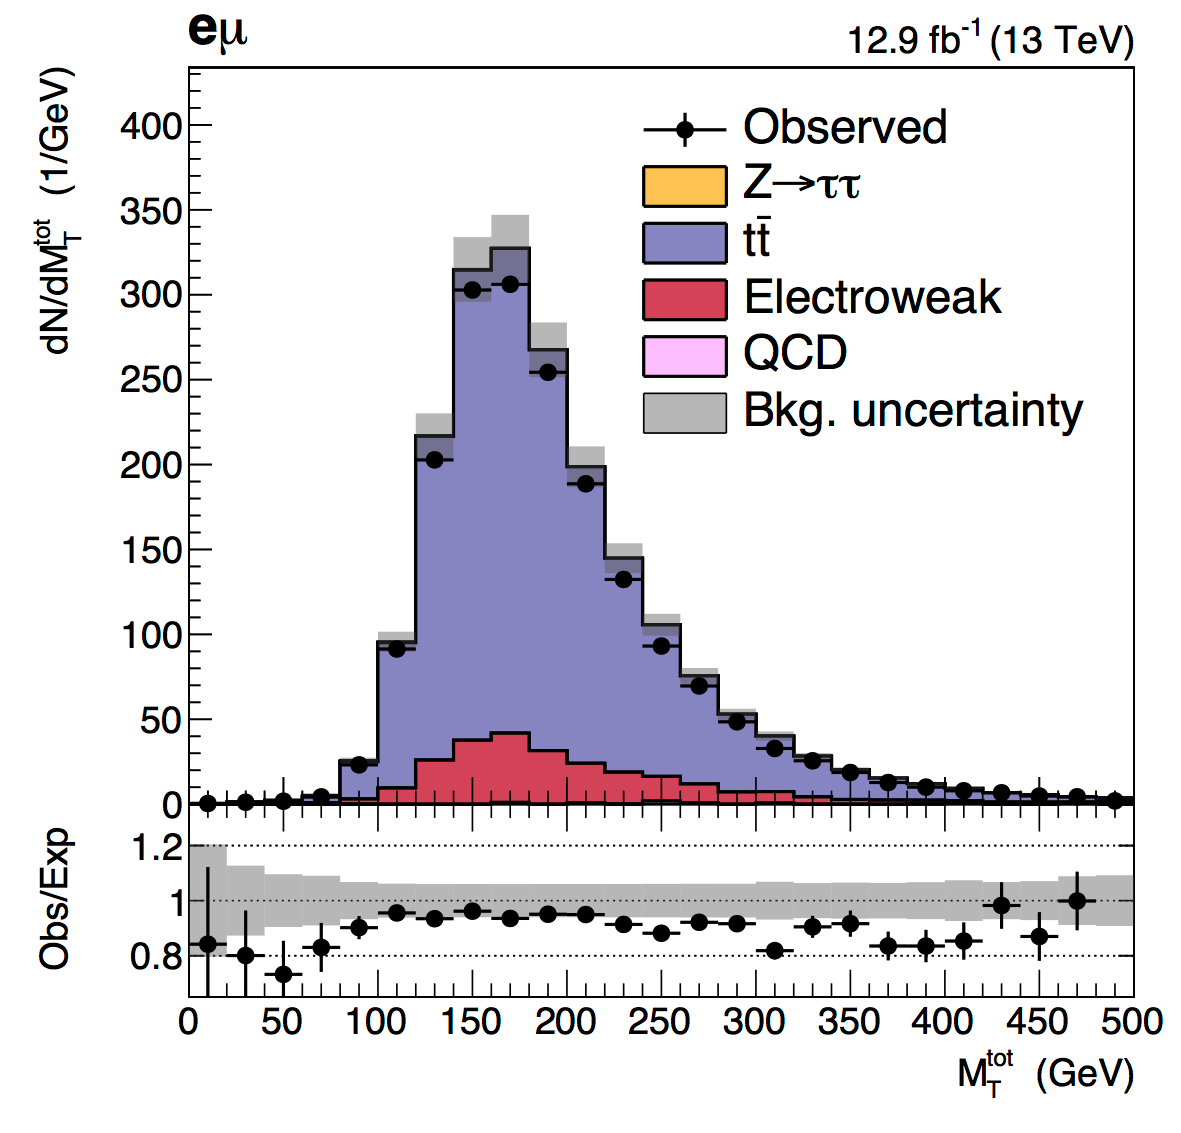
\includegraphics[width=0.5\textwidth]{./MSSM/Figures/mt_tot_ttcontrol_em_2016_notoppt.png}}
\subfloat[With top-quark \pT~reweighting]{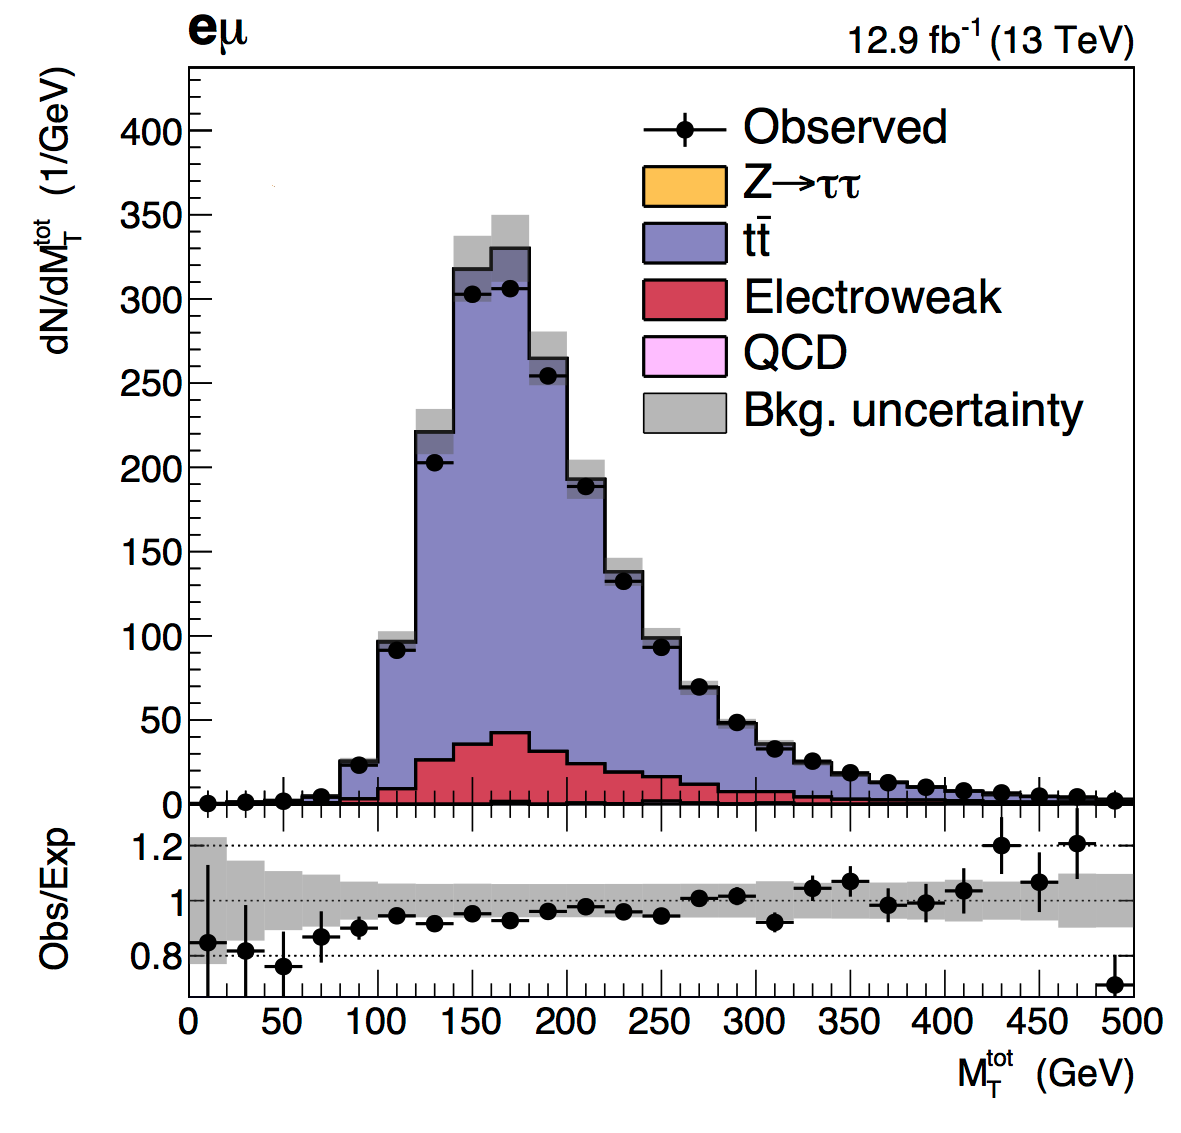
\includegraphics[width=0.5\textwidth]{./MSSM/Figures/mt_tot_ttcontrol_em_2016.png}}
\end{center}
\caption[\mTtot~distribution in the \ttbar
enriched control region, with and without applying top quark \pT~reweighting.]{\mTtot~distribution in the \ttbar enriched control region \MET>80 GeV and $D_{\zeta}<-20$ GeV in the \emu channel,
(a) without applying top quark \pT~reweighting and (b) with top quark \pT~reweighting.
The uncertainty band includes the statistical uncertainty as well as a 6\% \ttbar cross--section uncertainty.}
\label{fig:mssm_corrs_toppt}
\end{figure}

\subsubsection*{Drell-Yan shape reweighting}
As the \ac{MC} samples used for the \Ztautau estimate
do not model the data well for events with high di-lepton
mass and high Z \pT, a reweighting is applied to correct for this.
These weights are derived in bins of $\PZ/\Pphotonx$ mass and \pT~
using \Zmm events in data, in such a way that they do not
change the overall Drell-Yan normalisation. The weights
are then applied to the \Ztautau and \Zellell background processes.
The mismodelling can be seen in figure \ref{fig:dyrwt}a, which
shows the observed data and expected background distribution of the \PZ \pT~in
\Zmm events. The overall effect of the reweighting, which is derived
based on the events shown in figure \ref{fig:dyrwt}a, on the \Ztautau background
shape in the no b-tag category of the \etau channel is shown in figure \ref{fig:dyrwt}b.
\begin{figure}[h!]
\begin{center}
\subfloat[\Zmm events]{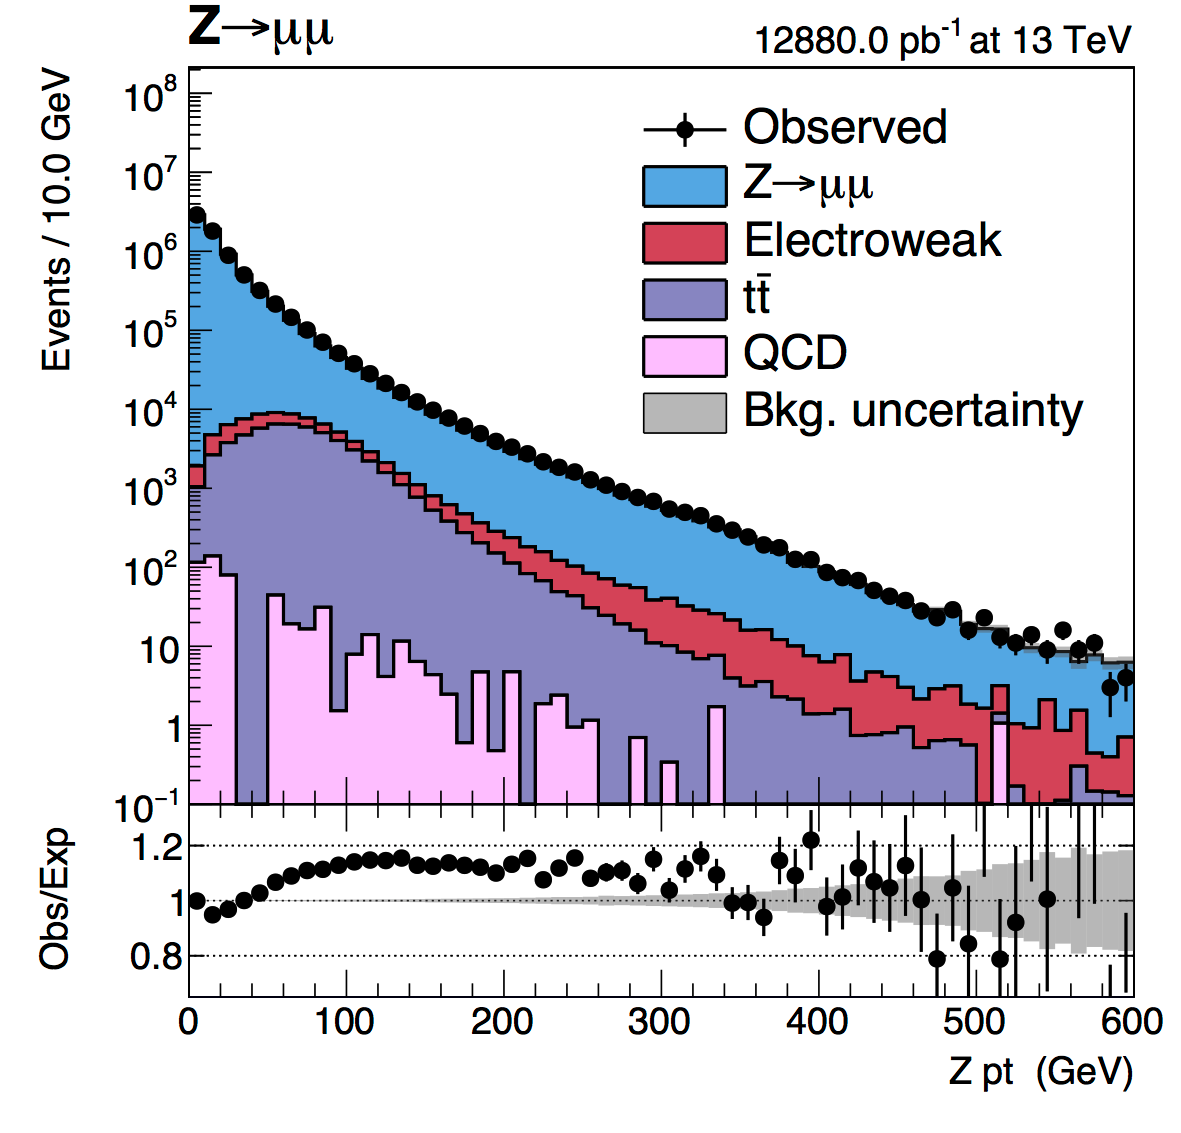
\includegraphics[width=0.5\textwidth]{./MSSM/Figures/pt_tt_inclusive_zmm_2016_log_noweight.png}}
\subfloat[Effect of Drell-Yan shape reweighting on \Ztautau background]{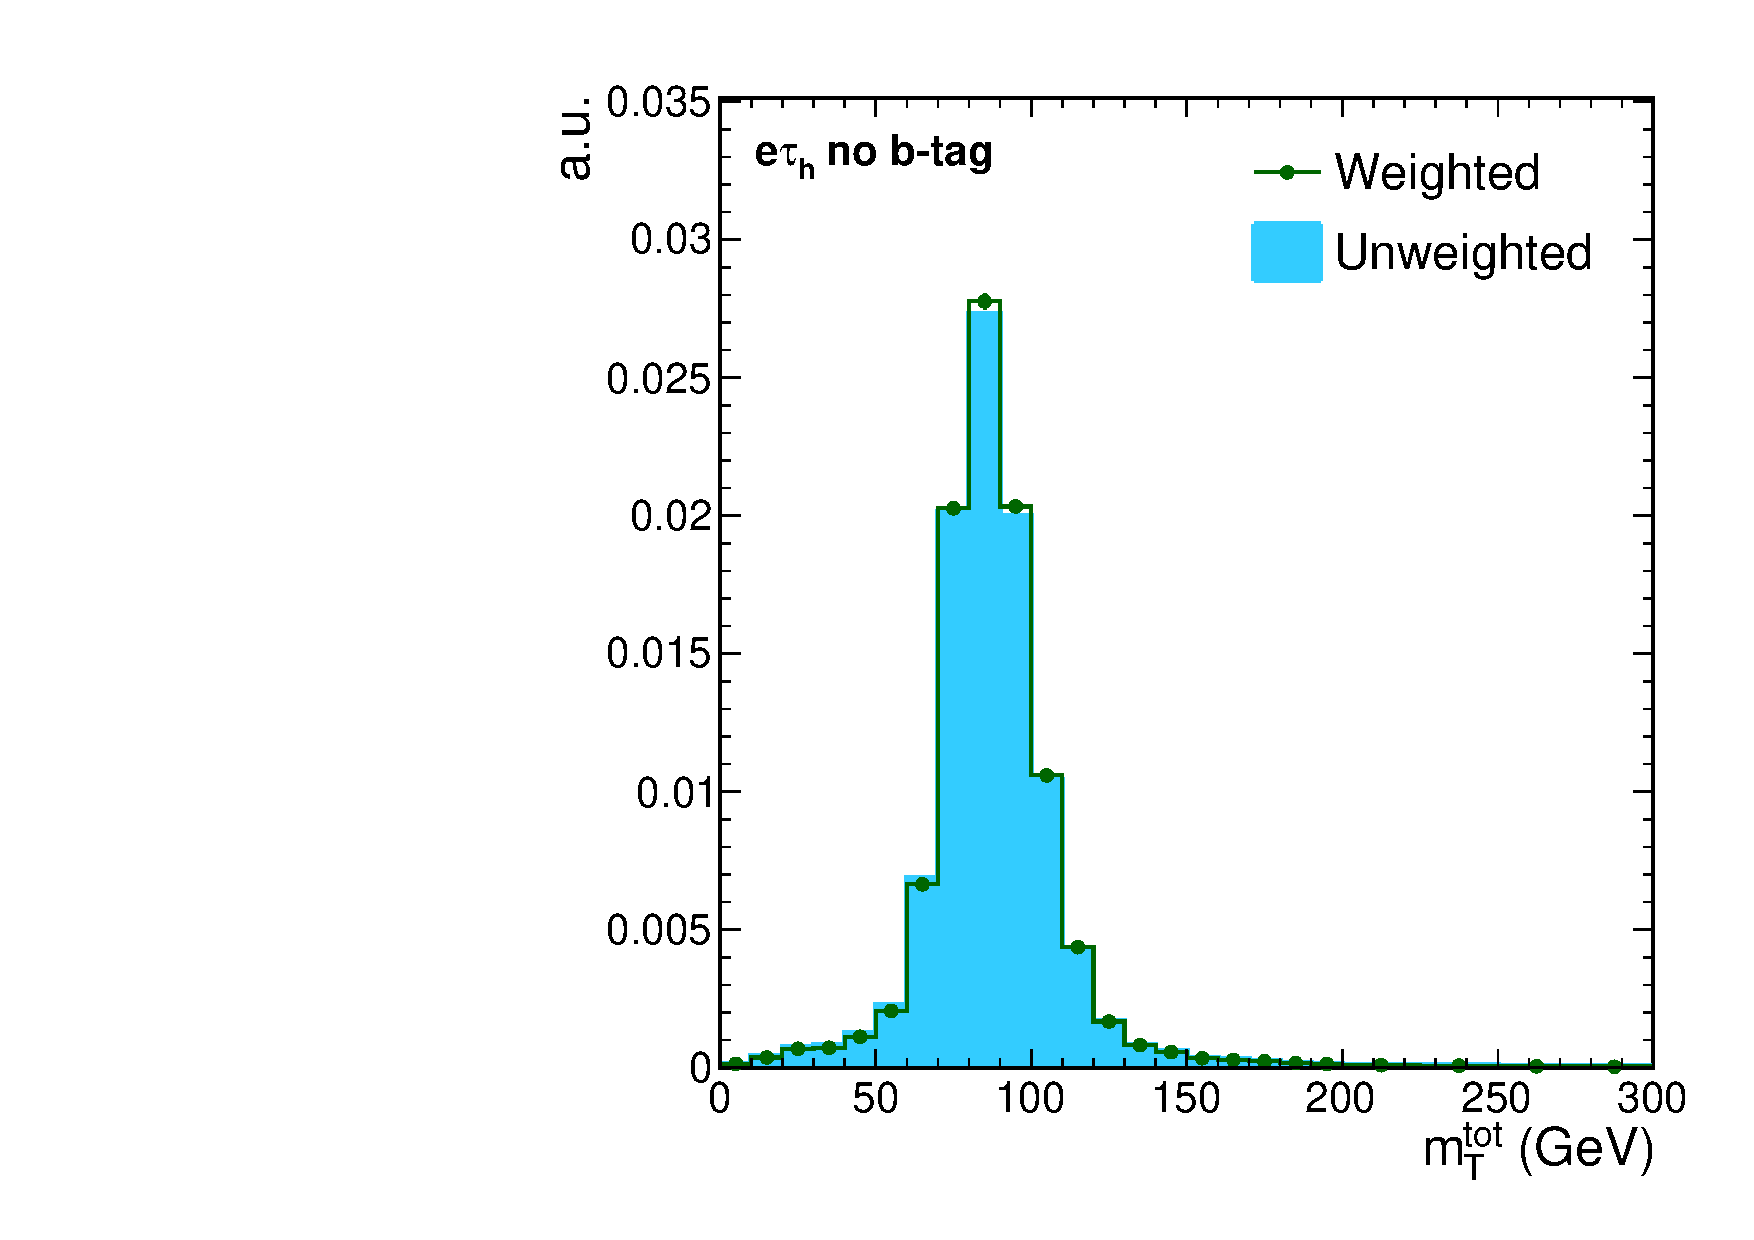
\includegraphics[width=0.5\textwidth]{./MSSM/Figures/mttot_zttweight_et_nobtag.pdf}}
\end{center}
\caption[The mismodelling in the \PZ \pT~distribution as observed
in \Zmm events, and the impact of applying the Drell-Yan shape reweighting
on the total transverse mass distribution of the \Ztautau background in the no b-tag category of the \etau channel.]{(a) The mismodelling in the \PZ \pT~distribution as observed
in \Zmm events, used to derive the correction and (b) the impact of applying the Drell-Yan shape
reweighting on the total transverse
mass distribution of the \Ztautau background in the no b-tag category of the \etau channel.}
\label{fig:dyrwt}
\end{figure}



\section{Background estimation}
\label{sec:mssm_bkgs}
There are several backgrounds in this analysis, and the different final
states can have different background compositions. Consider figure \ref{fig:mssm_bkgs_overview}a,
which shows the low $m_{\text{T}}^{\text{tot}}$ region in the no b-tag category
of the \mutau channel and figure \ref{fig:mssm_bkgs_overview}b, which shows the low $m_{\text{T}}^{\text{tot}}$
region in the b-tag category of the \emu channel. These regions are where the backgrounds are concentrated and it
is therefore easier to see the different contributions. \Ztautau is a background in all four channels as 
it has two real taus in the final state, like the signal that we are searching for. 
Smaller backgrounds 
from \Zellell decays also play a role, especially in the \mutau and \etau channels where such events
might pass the selection if for example a jet is misreconstructed as a hadronic tau and only one of the leptons is reconstructed. 
Production of QCD multijet events, labelled `QCD' on the plots in figure \ref{fig:mssm_bkgs_overview}, is a background when 
two jets are misreconstructed as the two particles of the candidate pair. %Relatively likely to happen in tautau channel
As visible in figure \ref{fig:mssm_bkgs_overview}b, the \ttbar background is particularly important in the b-tag category.
This is because top quarks virtually always decay as $\Ptop\rightarrow \PW\Pbottom$, and so such events nearly 
always contain real b-jets. The decay products  of one or both of the \PW bosons, and additional jets in the event, can 
then form \etau, \mutau, \tautau and \emu pairs.\\
The \Wjets process is a background in the \etau and \mutau channels when the lepton from the \PW decay and a jet misreconstructed
as a hadronic tau form a pair. In the \tautau channel it is a background when the \PW decays into $\Pgt\Pgn$ with the tau 
decaying hadronically and an additional jet in the event is misreconstructed as a hadronic tau, or when two jets are
reconstructed as hadronic taus.
In the \emu channel an additional lepton would have to originate from one of the jets, and so in this
channel this background is smaller. Backgrounds that are small in all channels are the di-boson and single-top backgrounds. In 
figures showing the backgrounds the di-boson and single-top backgrounds are drawn together with the \Wjets 
background as the `Electroweak' component.

\begin{figure}[h!]
\begin{center}
\subfloat[\mutau no b-tag]{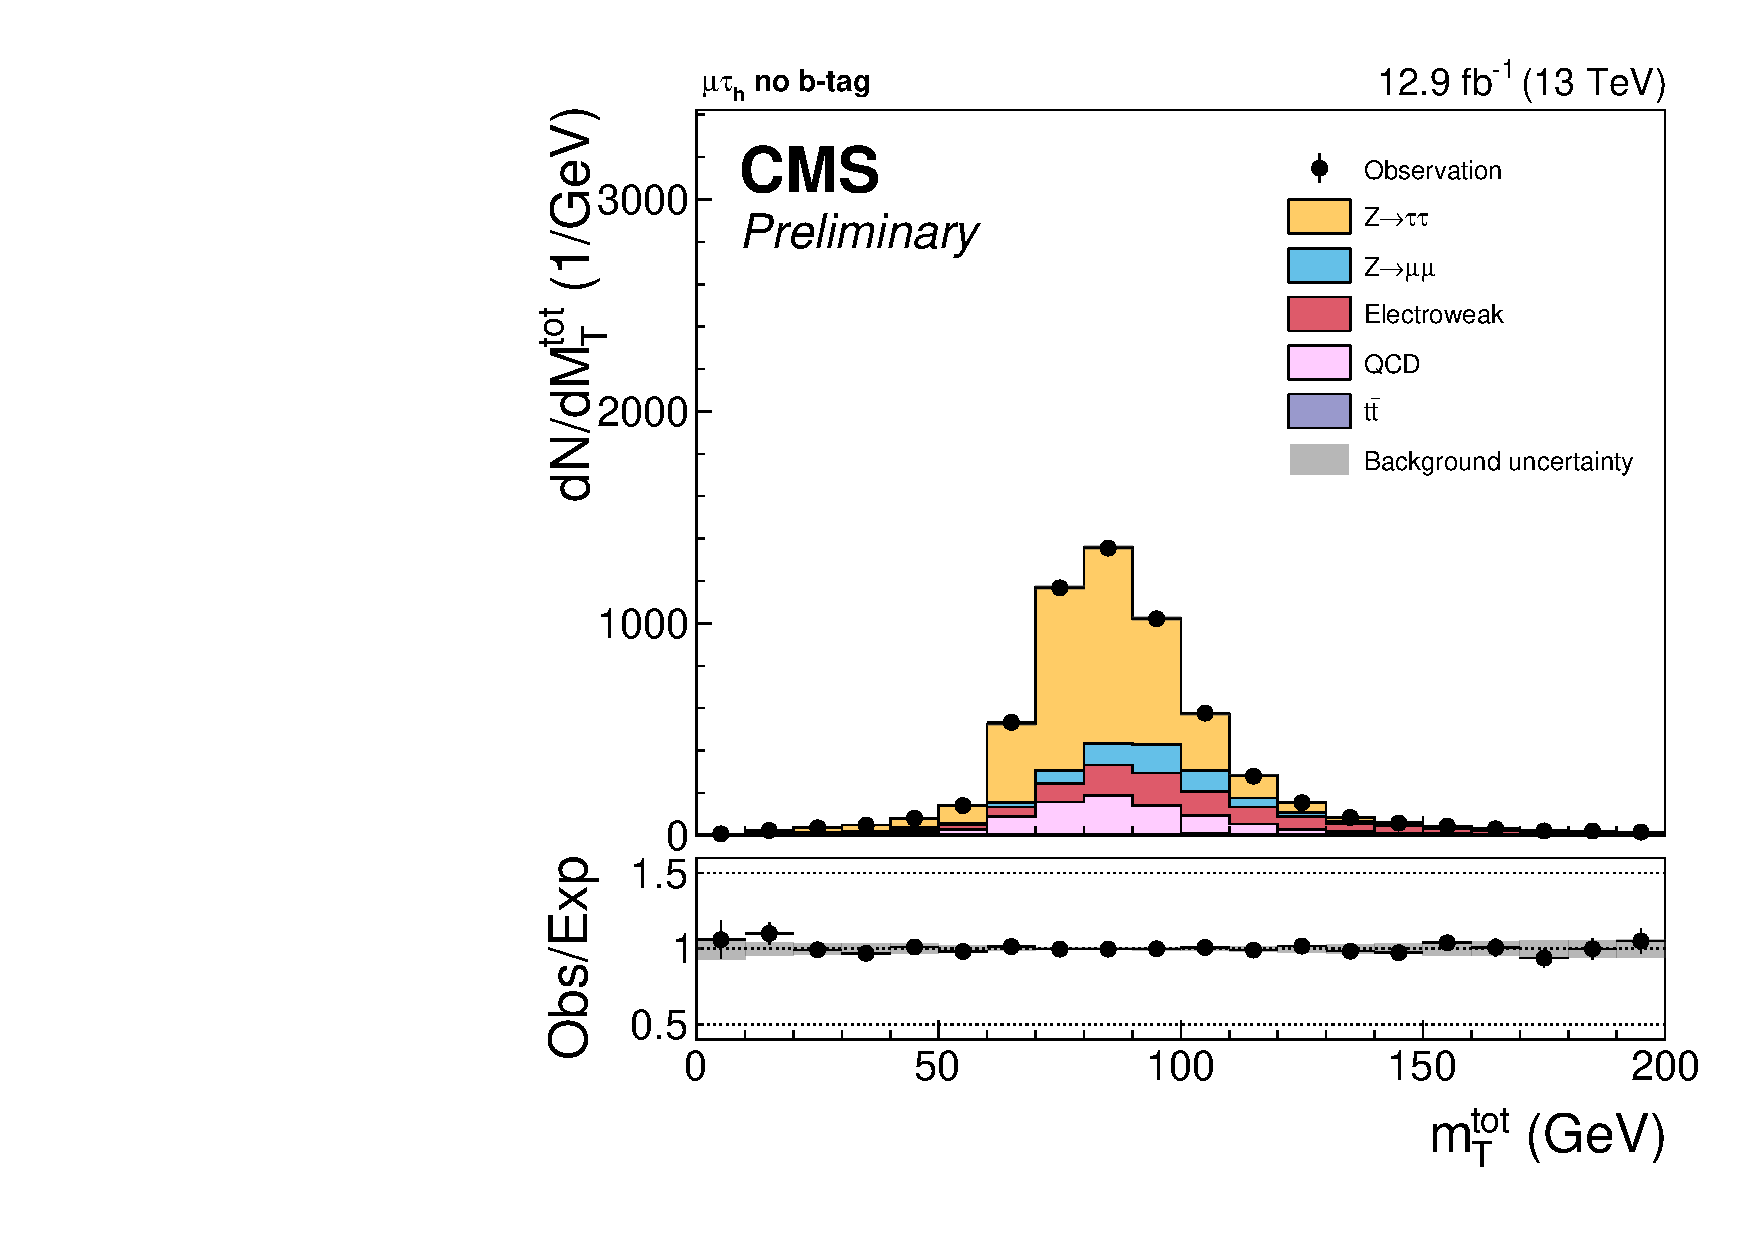
\includegraphics[width=0.5\textwidth]{./MSSM/Figures/CMS-PAS-HIG-16-037_Figure-aux_001-a.pdf}}
\subfloat[\emu b-tag]{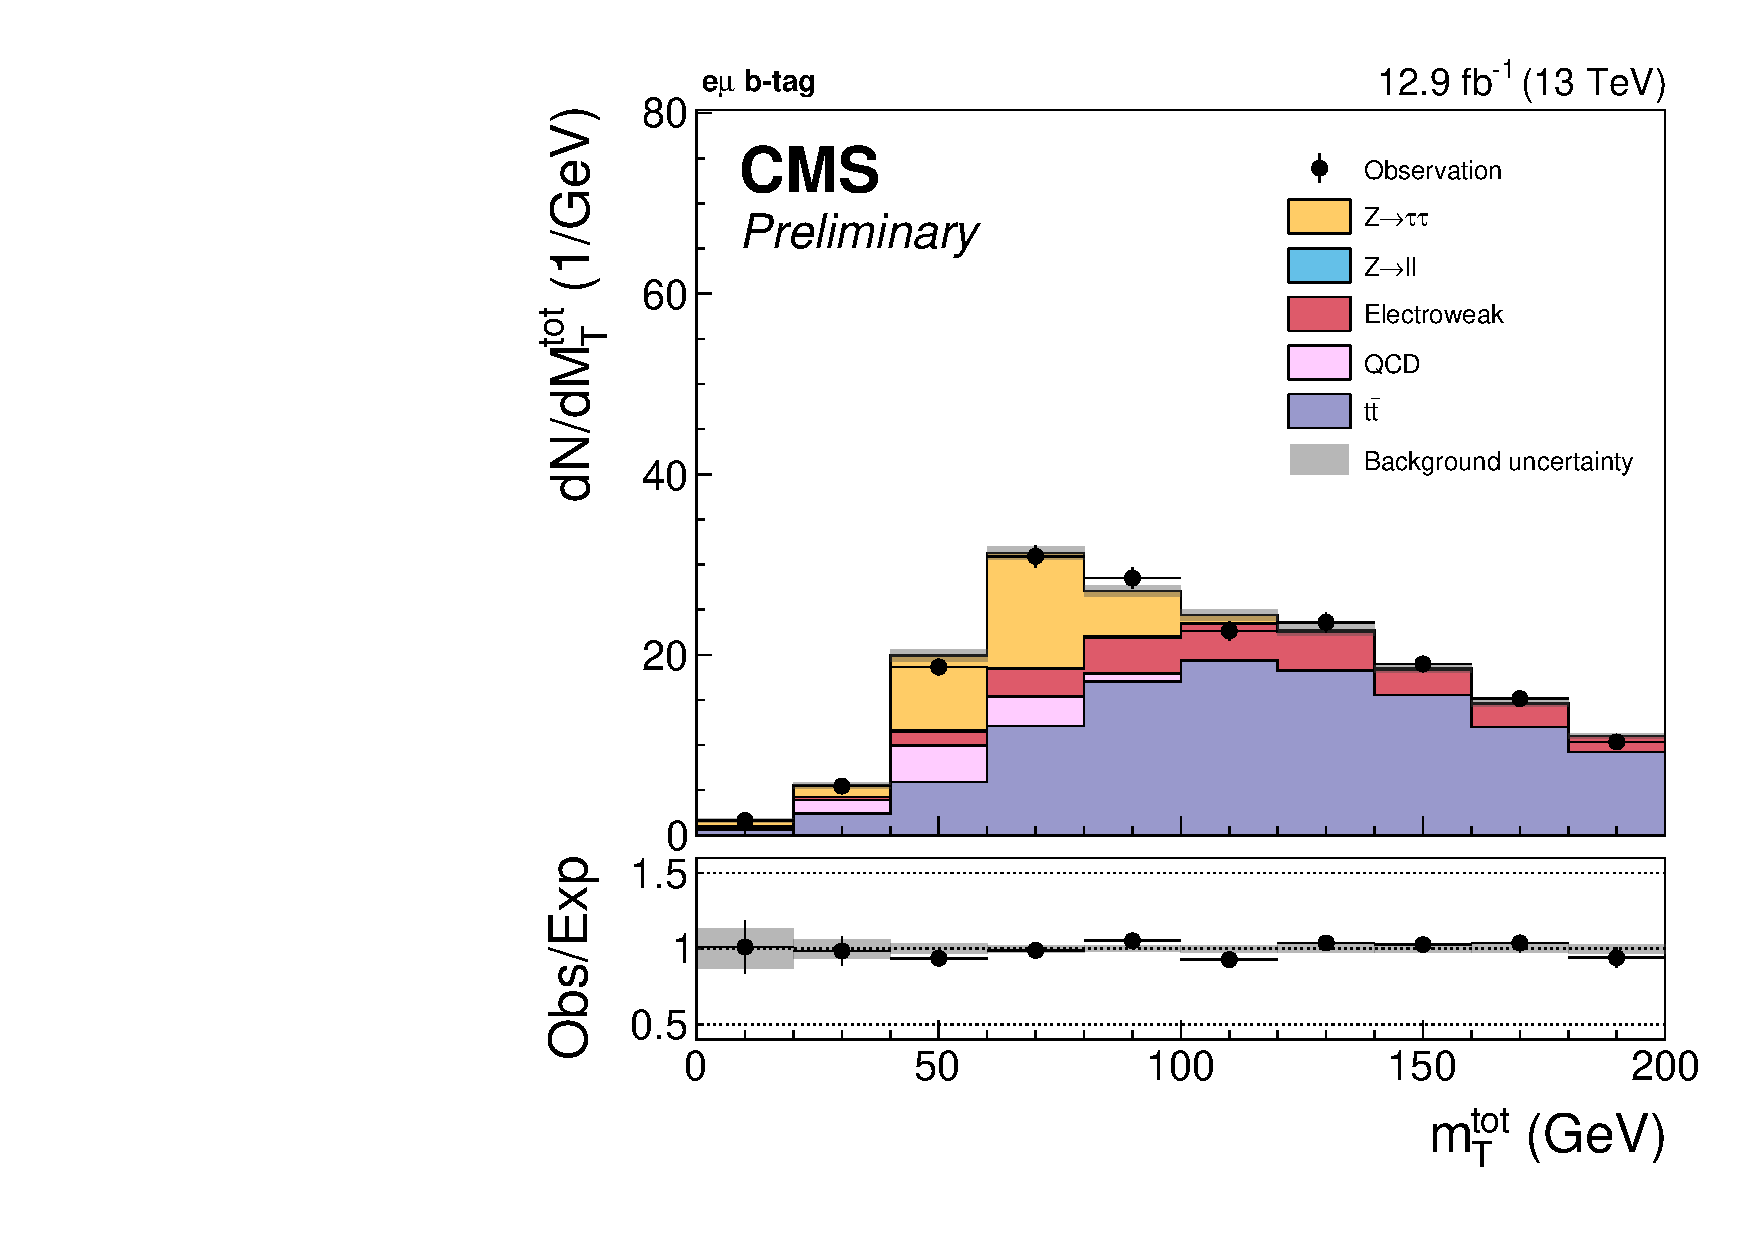
\includegraphics[width=0.5\textwidth]{./MSSM/Figures/CMS-PAS-HIG-16-037_Figure-aux_003-b.pdf}}
\end{center}
\caption[The low \mTtot~region in the no b-tag category of the \mutau channel 
and in the b-tag category of the \emu channel.]{The low $m_{\text{T}}^{\text{tot}}$ region in (a) the 
no b-tag category of the \mutau channel and (b) the b-tag category of the \emu channel.
This low $m_{\text{T}}^{\text{tot}}$ region is where the backgrounds
are concentrated \cite{CMS-PAS-HIG-16-037-addit}.}
\label{fig:mssm_bkgs_overview}
\end{figure}

To estimate these backgrounds a mixture of data-driven 
methods and \ac{MC} samples is employed. The QCD background
is estimated using data-driven techniques in all four channels.
In the \mutau and \etau channels the \Wjets background is also
estimated using data-driven techniques. The control regions used
for the estimation of QCD and \Wjets in the \etau and \mutau channels
are included in a simultaneous fit with the signal region to obtain
the final results. More detail on this is given in section \ref{sec:mssm_sigext_ctrl}.
In the \emu and \tautau channels the \Wjets background is estimated using
\ac{MC} samples. The \Ztautau and \Zellell backgrounds are estimated
using \ac{MC} samples for all four channels. A \Zmm control region
is considered in a simultaneous fit with the signal region to correct and
constrain the \Ztautau normalisation.
The \ttbar, di-boson and single-top backgrounds are estimated
using \ac{MC} samples, with cross-checks in control regions in data.
The rest of this section describes the background estimation methods
in more detail.

\subsection{Generator matching}
\label{sec:mssm_bkgs_genmatch}
For backgrounds estimated from \ac{MC}, it is possible
that it is more correct to split a background process
into different sub--processes that should be treated separately in the fit to data.
Taking the \mutau 
channel as an example, a sample of Drell--Yan events
will contain \Ztautau events, where one of the taus decays
hadronically and the other tau decays to a muon, but also
\Zmm events where one of the muons fakes a tau, or with an 
additional jet in the event faking a hadronic tau and one of the
muons not being properly reconstructed. Similarly, \ttbar background
events can be split into those with genuine taus, and those
where a jet mimics a hadronic tau. In such cases dividing
events from the same production process into sub--samples
based on generator information allows for a more correct
treatment of systematic uncertainties.

To determine the generator--level particle
that a reconstructed electron, muon, or hadronic tau
originates from, reconstructed objects are matched
to a set of generator level objects within a cone of $\Delta R = 0.2$.
Five categories of generator-level object are considered for matching:
prompt electrons and muons,
that is electrons and muons not originating from a hadron, tau or muon decay; electrons and muons
from tau decays; and generator-level hadronic taus. These generator-level
hadronic taus are rebuilt by summing the four--momenta
of the visible decay products of the generator-level tau.

If there is at least one generator-level object
within a cone of $\Delta R = 0.2$ around the direction of the reconstructed
object, the generator-level object nearest the reconstructed particle is chosen
as the one the reconstructed particle is matched to. 
If there are no 
generator-level particles in the cone at all it is said to 
have originated from pile--up or a jet at generator level.

The generator--level object type matched to a 
reconstructed particle is used to perform the splitting
of background samples, where this is used it is indicated.

\subsection{\texorpdfstring{\Ztautau}{Z to tau tau}}
\label{sec:mssm_bkgs_ztt}
For all channels, both shape and normalisation of the \Ztautau background 
are estimated from the Drell-Yan
\ac{MC} samples described in section \ref{sec:mssm_datasets}.
For the \mutau and \etau channels, events from these samples 
in which the reconstructed hadronic tau is matched to 
a generator-level hadronic tau are considered part of the \Ztautau
background. In the \tautau channel both reconstructed
hadronic taus are required to be matched to a generator-level hadronic tau, and
in the \emu channel the \Ztautau component of the Drell-Yan background 
is taken as those events where the reconstructed electron is not matched to
a prompt electron at generator level and the reconstructed
muon is not matched to a prompt muon. 
Events in the Drell-Yan samples selected in the event selection
but not satisfying the generator matching requirements are considered
as the, much smaller, \Zll background.

To correct and constrain the \Ztautau normalisation in the
b-tag and no b-tag categories of all channels, \Zmm control
regions are considered in a simultaneous fit with the signal region. More detail is given in 
section \ref{sec:mssm_sigext_ctrl}.

\subsection{\texorpdfstring{\Wjets and QCD in the \etau and \mutau channels}{W+jets and QCD in the e tau and mu tau channels}}
\label{sec:mssm_bkgs_mtet_wjetsqcd}
A data--driven approach is used for the estimation of
both the \Wjets and QCD backgrounds in the \etau and \mutau channels. 
The estimates of the normalisations of the two backgrounds are tied
together due to the presence of some QCD contamination in the \Wjets--dominated
control region. The shape of the \Wjets background is taken
from the \ac{MC} samples. The QCD shape taken from same--sign
data, that is events selected in observed data with the opposite charge requirement
on the di-$\Pgt$ pair inverted but otherwise identical cuts to the signal region. Contributions
from other backgrounds in this region are subtracted.

\subsubsection{\texorpdfstring{\Wjets normalisation}{W+jets normalisation}}
\label{sec:mssm_bkgs_mtet_wjetsnorm}
The \Wjets normalisation is derived using a high-\mT~ control region, where
selected events are required to satisfy \mT$>70$ GeV. The 
\Wjets
contribution in this region is enhanced, however there is still
some contribution from QCD events in this region. This is visible in 
figure \ref{fig:mssm_bkgs_wjets_mutau_mt} which shows the \mT~distribution in the
\mutau channel, indicating the signal region and the high-\mT~control region. 

\begin{figure}[h!]
\begin{center}
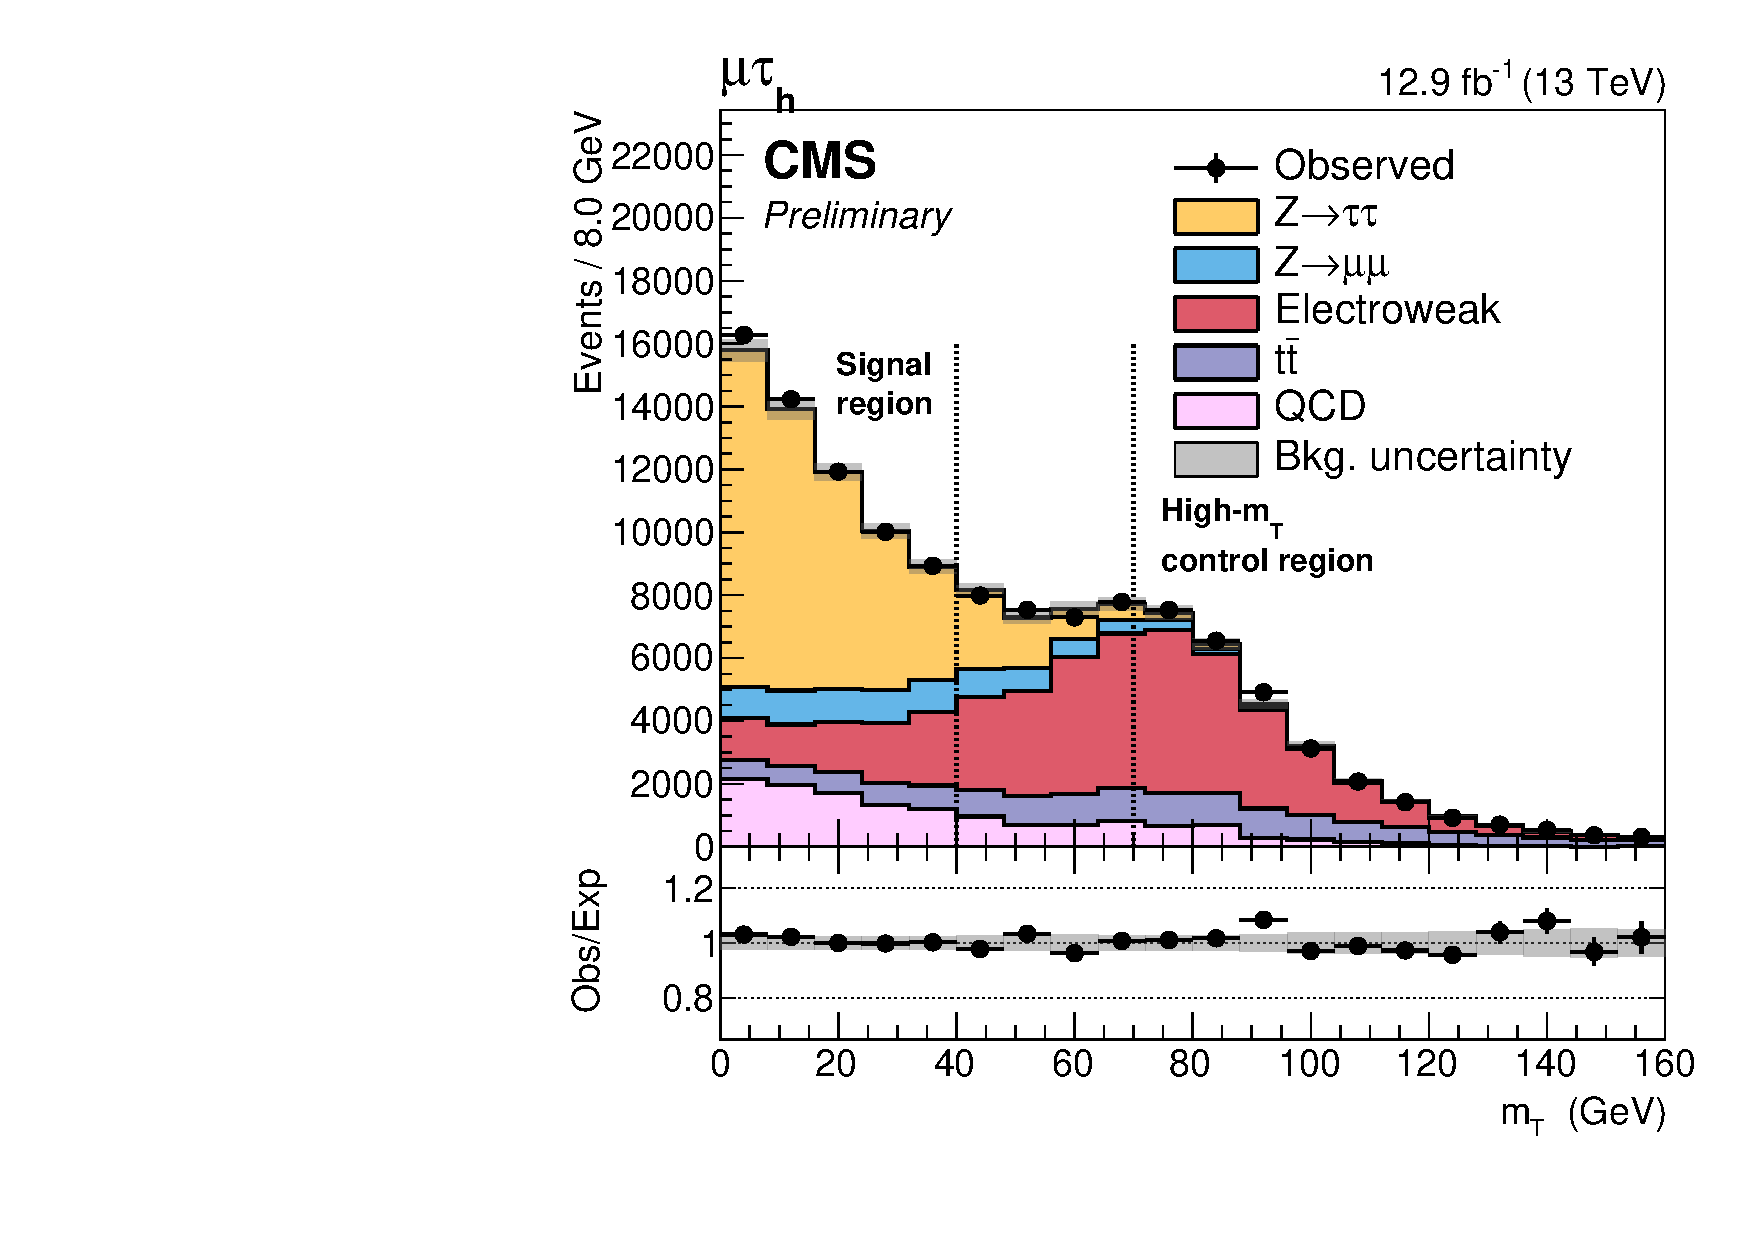
\includegraphics[width=0.5\textwidth]{./MSSM/Figures/CMS-PAS-HIG-16-037_Figure_002.pdf}
\end{center}
\caption{Distribution of the transverse mass \mT~in the \mutau channel, indicating
the signal region and the high \mT~control region. This distribution is plotted
before dividing the events into categories \cite{CMS-PAS-HIG-16-037}.}
\label{fig:mssm_bkgs_wjets_mutau_mt}
\end{figure}

Because of this contribution from QCD events in the high \mT~region we
have, for \mT$>70$ GeV:
\begin{equation}\label{eqn:wjets_ss_norm}
\begin{split}
&N_{\text{data}}^{\text{SS, high } m_{\text{T}}} - N_{\text{other}}^{\text{SS,
 high } m_{\text{T}}}  =
N_{\text{QCD}}^{\text{SS, high } m_{\text{T}}} + N_{\text{W}}^{\text{SS, high } m_{\text{T}}} ~\\
&N_{\text{data}}^{\text{OS, high } m_{\text{T}}} - N_{\text{other}}^{\text{OS,
 high } m_{\text{T}}}  = N_{\text{QCD}}^{\text{OS, high } m_{\text{T}}} +
N_{\text{W}}^{\text{OS, high } m_{\text{T}}} \\
& = R_{\text{QCD}}^{\text{OS/SS}}\cdot N_{\text{QCD}}^{\text{SS, high } m_{\text{T}}} +
R_{\text{W}}^{\text{OS/SS}} \cdot N_{\text{W}}^{\text{SS, high } m_{\text{T}}} ~\\
&\Rightarrow N_{\text{W}}^{\text{SS, high } m_{\text{T}}}  = \frac{N_{\text{data}}^{\text{OS,
 high } m_{\text{T}}}  - N_{\text{other}}^{\text{OS, high } m_{\text{T}}}  -
R_{\text{QCD}}^{\text{OS/SS}}\cdot(N_{\text{data}}^{\text{SS, high } m_{\text{T}}}  -
N_{\text{other}}^{\text{SS, high } m_{\text{T}}} )}{R_{\text{W}}^{\text{OS/SS}} -
R_{\text{QCD}}^{\text{OS/SS}}} ,
\end{split}
\end{equation}
where $R_{\text{W}}^{\text{OS/SS}}$ is the ratio between opposite-sign and same-sign \Wjets events
and $R_{\text{QCD}}^{\text{OS/SS}}$ the ratio between opposite-sign and same-sign QCD events. Using 
equation \ref{eqn:wjets_ss_norm}, the number of \Wjets events in the
opposite-sign, high \mT~region is given by $R_{\text{W}}^{\text{OS/SS}}\cdot N_{\text{W}}^{\text{SS, high } m_{T}}$. 
This is extrapolated to the number of \Wjets events in the signal region at low \mT~as:
\begin{equation}\label{eqn:wjets_os_norm}
N_{\text{W}}^{\text{OS, low} m_{T}} = \frac{N_{\text{W,MC}}^{\text{OS, low} m_{T}}}{N_{\text{W,MC}}^{\text{OS, high} m_{T}}}\cdot R_{\text{W}}^{\text{OS/SS}} \cdot N_{\text{W}}^{\text{SS, high }m_{T}},
\end{equation}
which means the estimate of the number of \Wjets events in the opposite-sign, high \mT, region
is multiplied by a high \mT-to-low \mT~extrapolation factor determined from the \ac{MC} samples.

The use of the method presented relies on knowledge of $R_{\text{W}}^{\text{OS/SS}}$,
$R_{\text{QCD}}^{\text{OS/SS}}$, and on these two ratios not being too similar to each other. 
The ratio $R_{\text{QCD}}^{\text{OS/SS}}$ is measured in an anti--isolated
control region in data; this measurement is described in section \ref{sec:mssm_bkgs_etmt_qcdosss}. $R_{\text{W}}^{\text{OS/SS}}$ is 
taken from the \Wjets \ac{MC} samples, and is found to be between 4 and 5, while $R_{\text{QCD}}^{\text{OS/SS}}$
is close to 1.

The method described so far works well in the no b-tag categories, but in the b-tag category of both channels
the \ttbar background dominates. This is illustrated in figure \ref{fig:bkgs_highmtctrl}, where
the high-\mT~region in the no b-tag category (figure \ref{fig:bkgs_highmtctrl}a) is compared with the high-\mT~region in the 
b-tag category (figure \ref{fig:bkgs_highmtctrl}b) of the \etau channel. It is clear that the \ttbar 
background is much larger than the \Wjets background in the b-tag high-\mT~control region.
For this reason the estimate of the number
of \Wjets events in this category is made with a relaxed category selection where the b-tagging
requirement itself is removed, but the jet requirements still stand. Events with at least one 
jet with \pT$>20$ GeV and with $|\eta|<2.4$, but at most one jet with \pT$>30$ GeV and $|\eta|<4.7$, are therefore selected. The final \Wjets estimate in the b-tag category signal
region is determined by the estimate given by the number of \Wjets events
estimated in the 1-jet selection, multiplied by an extrapolation factor 
$\frac{N_{\text{W,MC}}^{\text{OS,low } m_{T},\text{b-tag category}}}{N_{\text{W,MC}}^{\text{OS, low }m_{\text{T}},\text{1-jet selection}}}$.
\begin{figure}[h!]
\begin{center}
\subfloat[No b-tag]{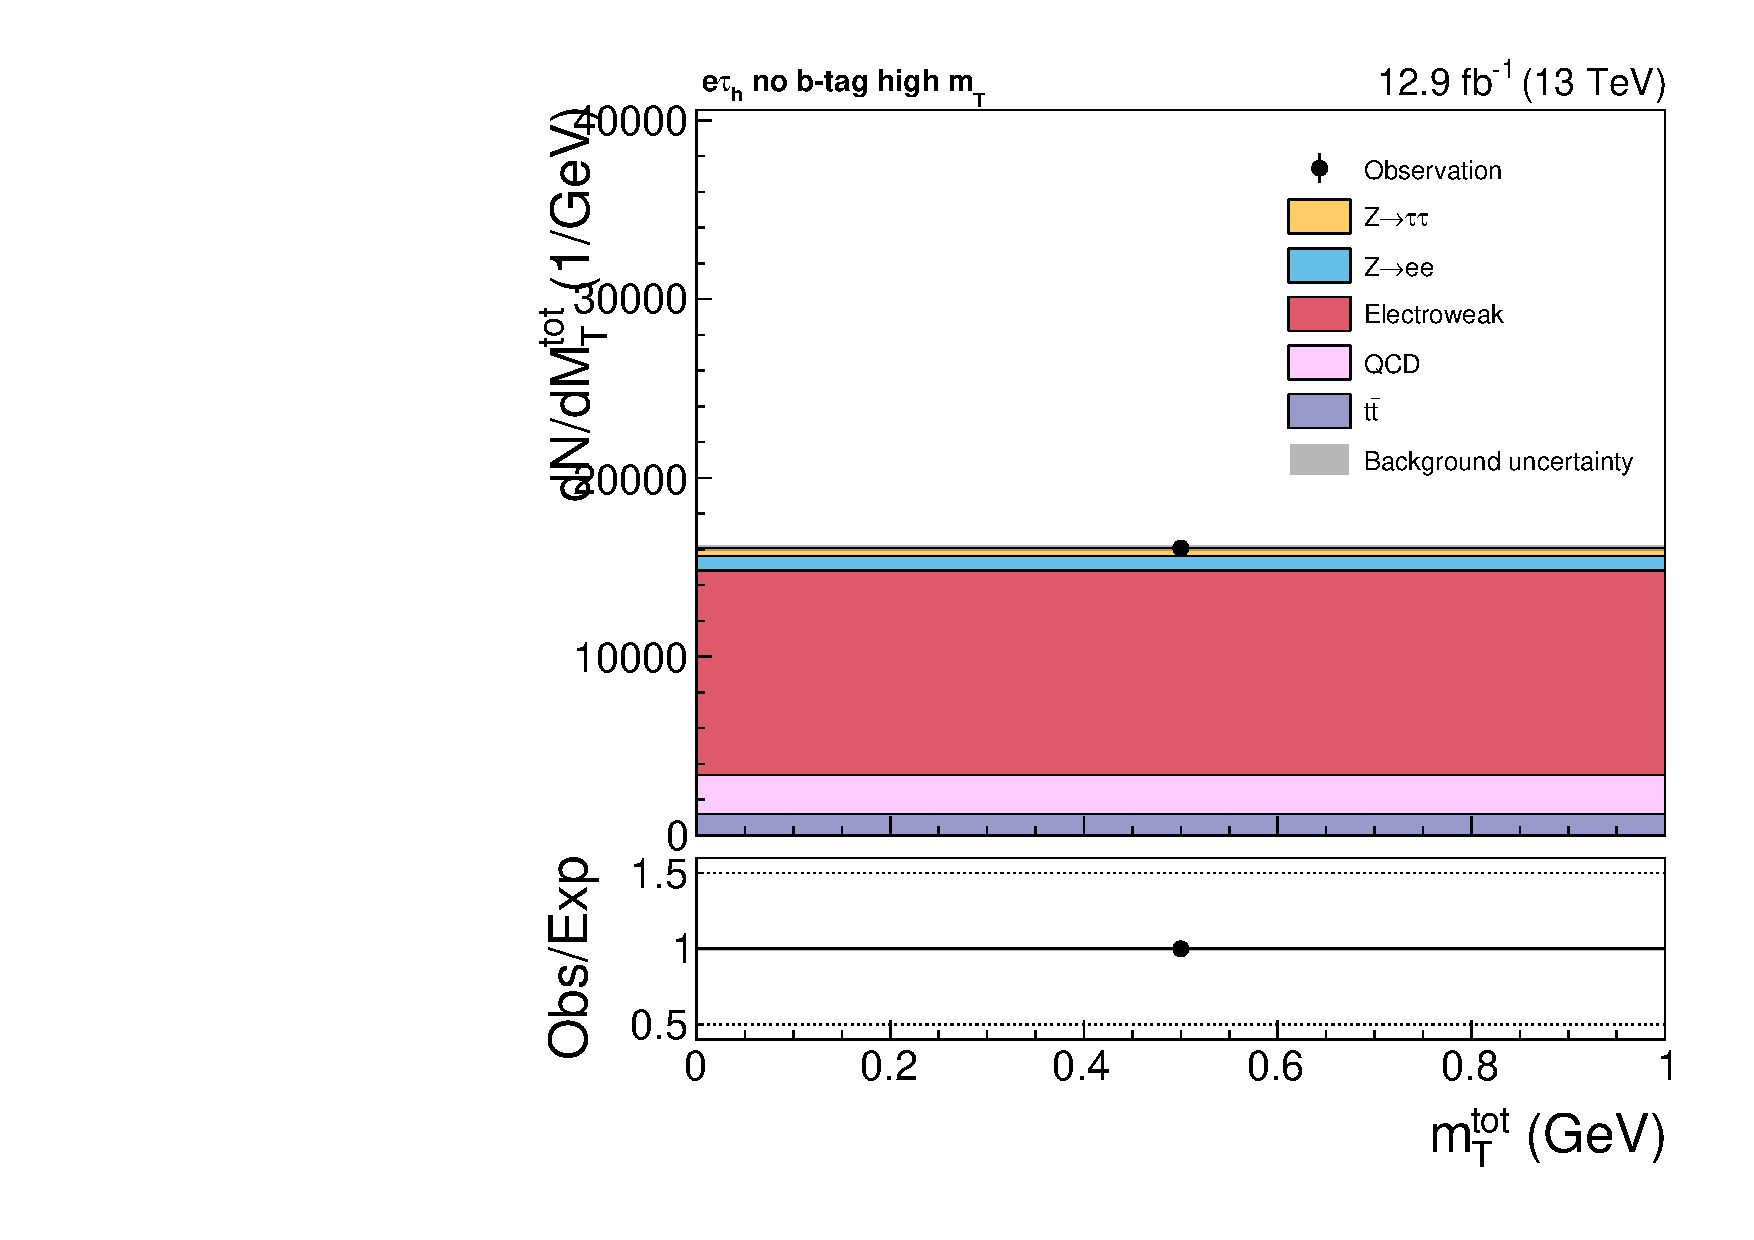
\includegraphics[width=0.5\textwidth]{./MSSM/Figures/htt_et_10_shapes_postfit.pdf}}
\subfloat[B-tag]{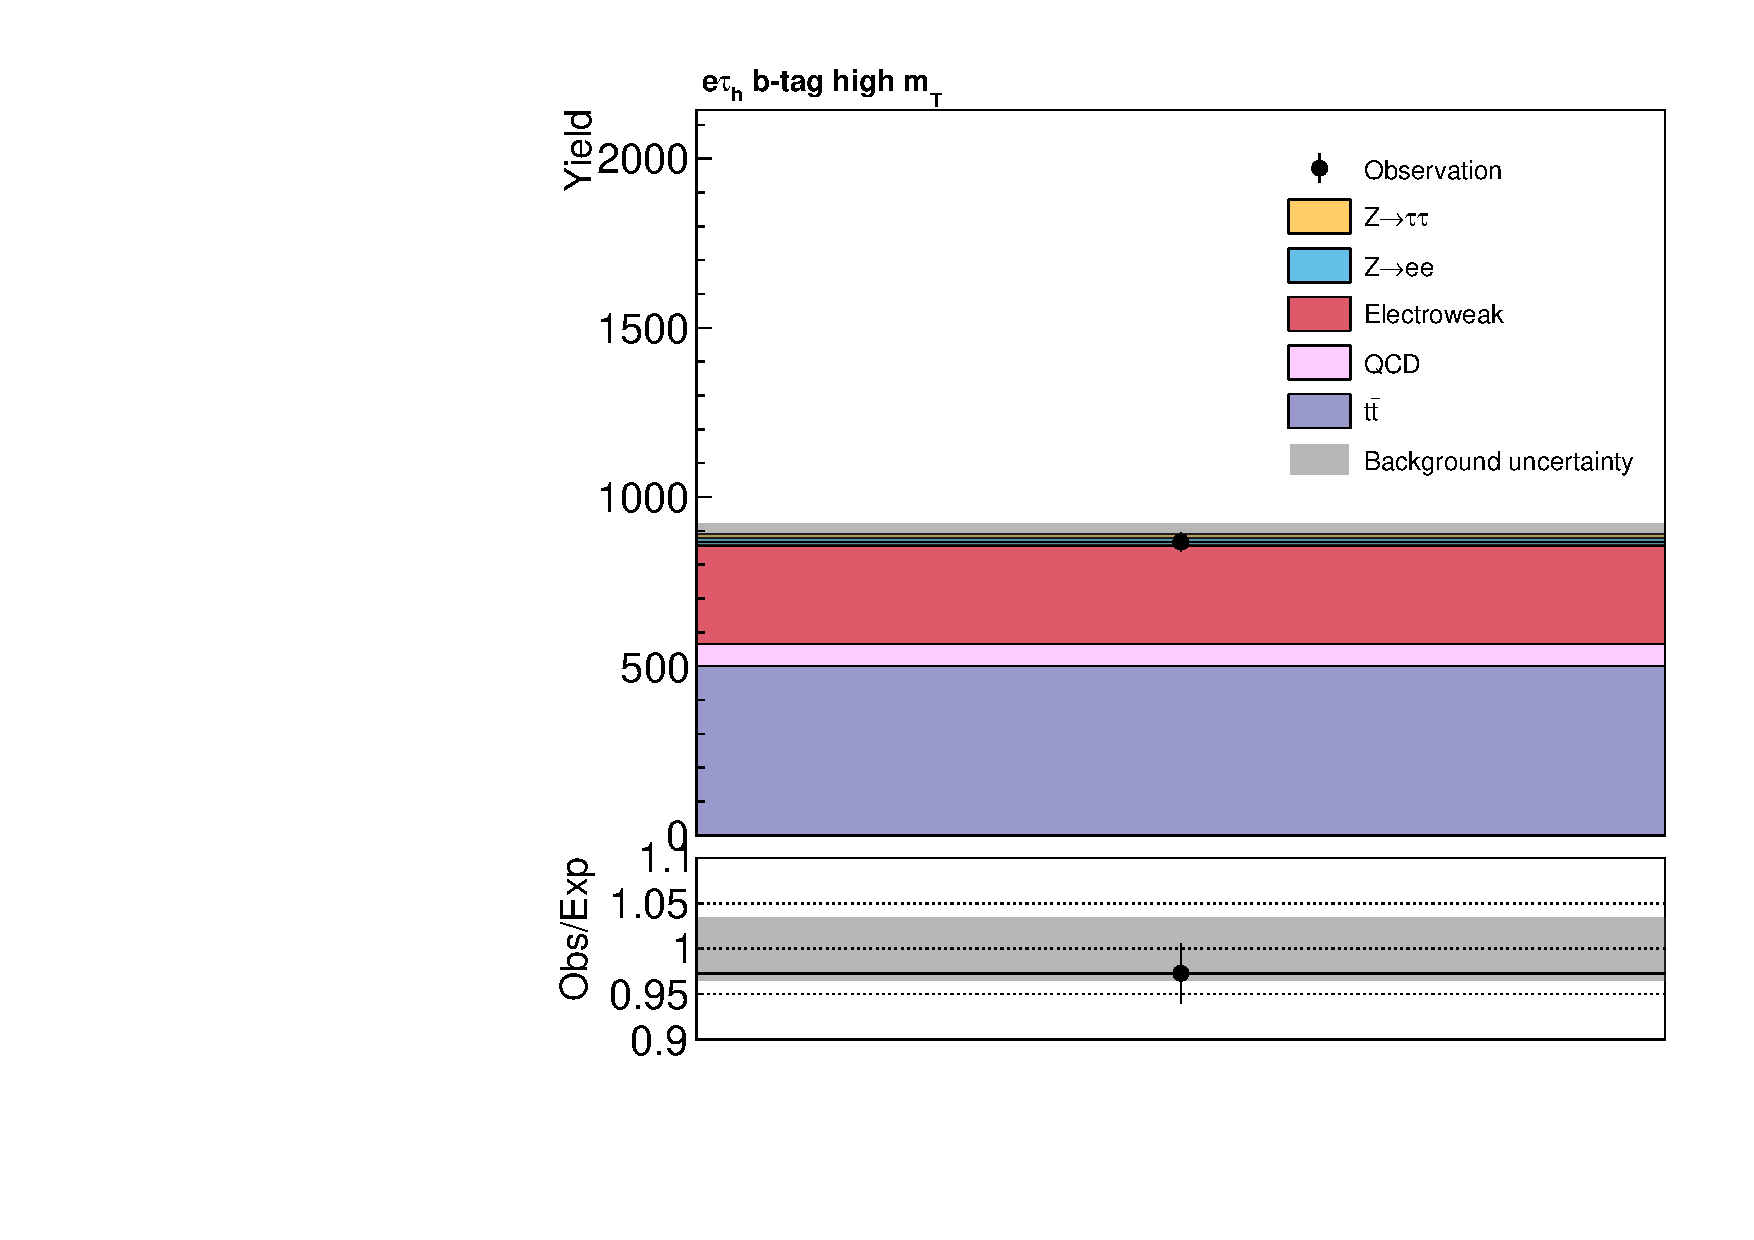
\includegraphics[width=0.5\textwidth]{./MSSM/Figures/htt_et_13_shapes_postfit.pdf}}
\end{center}
\caption[High-\mT~control region in the no b-tag and b-tag
categories of the \etau channel.]{High-\mT~control region in the (a) no b-tag and (b) b-tag categories of the \etau
channel. In the no b-tag category the \Wjets background, drawn together with the small
 di-boson plus single-top backgrounds as the `electroweak' background component, dominates. In the b-tag
category the \ttbar background is larger than the \Wjets background.}
\label{fig:bkgs_highmtctrl}
\end{figure}

\subsubsection{QCD OS/SS ratio}
\label{sec:mssm_bkgs_etmt_qcdosss}
The ratio of opposite--sign to same--sign QCD events, $R_{\text{QCD}}^{\text{OS/SS}}$, is measured
in two anti-isolated sidebands by performing a fit to the distribution of the
visible mass of the di-tau pair in 
opposite-sign events. The QCD template, which is taken from same--sign events 
assuming $R_{\text{QCD}}^{\text{OS/SS}} = 1$ is treated as the signal, and a binned maximum
likelihood fit to the QCD signal strength is performed while allowing the other
backgrounds to float within reasonable normalisation uncertainties. The
resulting best fit value of the signal strengh parameter is taken as $R_{\text{QCD}}^{\text{OS/SS}}$.
Of the two sidebands used, one is nearer the signal region ($0.15<I_{\text{rel}}^{\Pgm}<0.25$ for the \mutau channel and $0.1<I_{\text{rel}}^{\Pe}<0.2$ for the \etau channel)
and one further away ($0.25<I_{\text{rel}}^{\Pgm}<0.5$ for the \mutau channel and $0.2<I_{\text{rel}}^{\Pe}<0.5$ for the \etau channel). The results of the fits,
performed before the categorisation of events into the b-tag and no b-tag categories, are shown in figures \ref{fig:mssm_qcdosss_mtnear} and \ref{fig:mssm_qcdosss_mtfar}
for the \mutau channel and in figures \ref{fig:mssm_qcdosss_etnear} and \ref{fig:mssm_qcdosss_etfar} for the \etau channel.
The value of $R_{\text{QCD}}^{\text{OS/SS}}$ is found to be consistent between the two sidebands within 10\% (1\%) in the \etau (\mutau) channel.
Adding this uncertainty in quadrature to the uncertainty on the fit in the sidebands nearest the signal region we find
an overall uncertainty of 12\% in the \etau channel and 4\% in the \mutau channel.
When performing the same fits in the no b-tag and b-tag categories to determine differences between
this pre-categorisation opposite--sign to same--sign ratio, and the ratio as measured in categories it is found that 
the fit is not stable in the b-tag category due to the number of events in this region being too small.
The uncertainty on the ratio is increased for the b-tag category to cover the differences.
The uncertainties are already large enough to cover differences between the pre-categorisation $R_{\text{QCD}}^{\text{OS/SS}}$ and the
fits as performed in the no b-tag category. Therefore $R_{\text{QCD}}^{\text{OS/SS}}$ in the \mutau channel is taken to be
1.18 in both the b-tag and the no b-tag category, with a 60\% uncertainty in the b-tag category and a 4\% uncertainty in the no b-tag category.
In the \etau channel $R_{\text{QCD}}^{\text{OS/SS}}$ is taken to be 1.02 with a 60\% uncertainty in the b-tag category and a 12\% uncertainty
in the no b-tag category.

\begin{figure}[h!]
\begin{center}
\subfloat[Pre-fit distribution]{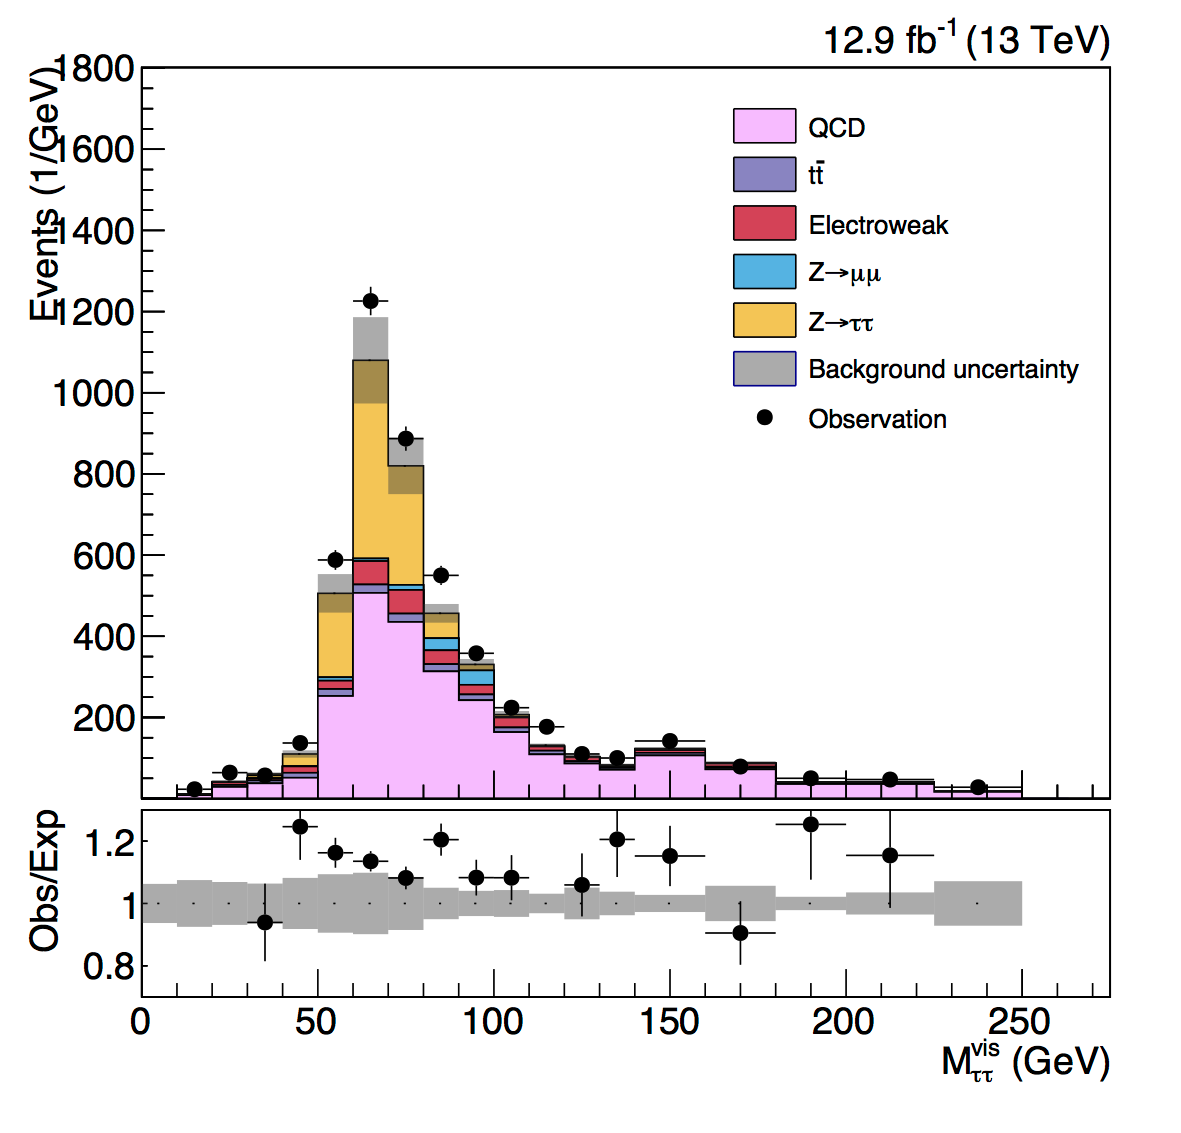
\includegraphics[width=0.5\textwidth]{./MSSM/Figures/qcdosss_near_mt_1_prefit.png}}
\subfloat[Post-fit distribution]{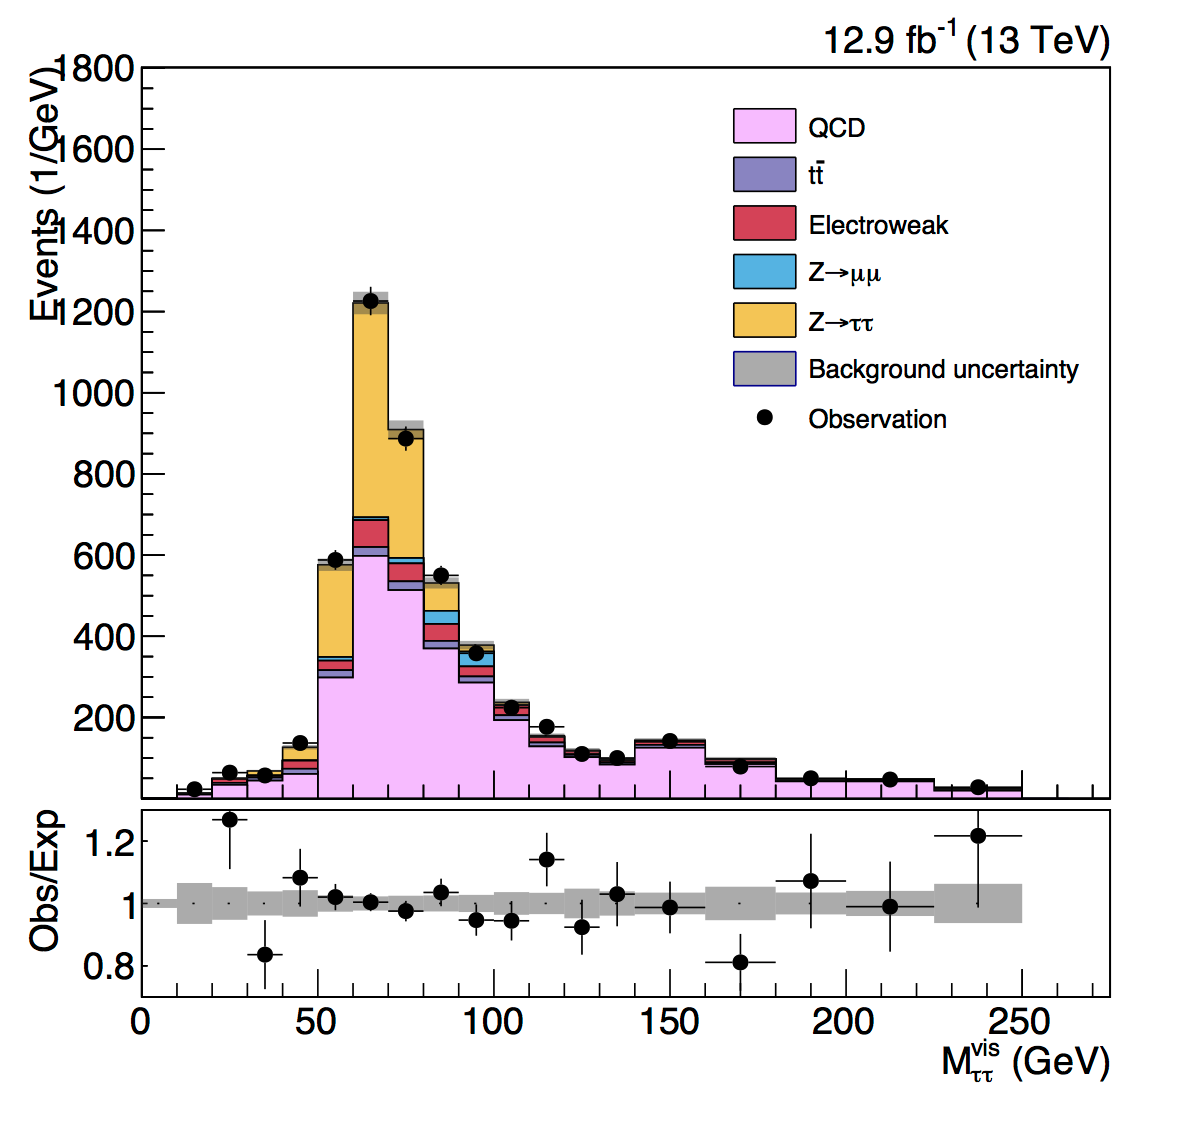
\includegraphics[width=0.5\textwidth]{./MSSM/Figures/qcdosss_near_mt_1_postfit.png}}
\end{center}
\caption[The visible mass distribution of the di-$\tau$ pair
in the \mutau channel for the sideband near the signal region, before
and after the maximum likelihood fit to the QCD signal strength.]{The visible mass distribution of the di-$\tau$ pair in the \mutau channel for the sideband near the signal region, (a) before
the maximum likelihood fit to the QCD signal strenght and (b) after the fit. The resulting fitted signal strength 
is 1.180$\pm$0.044.}
\label{fig:mssm_qcdosss_mtnear}
\end{figure}

\begin{figure}[h!]
\begin{center}
\subfloat[Pre-fit distribution]{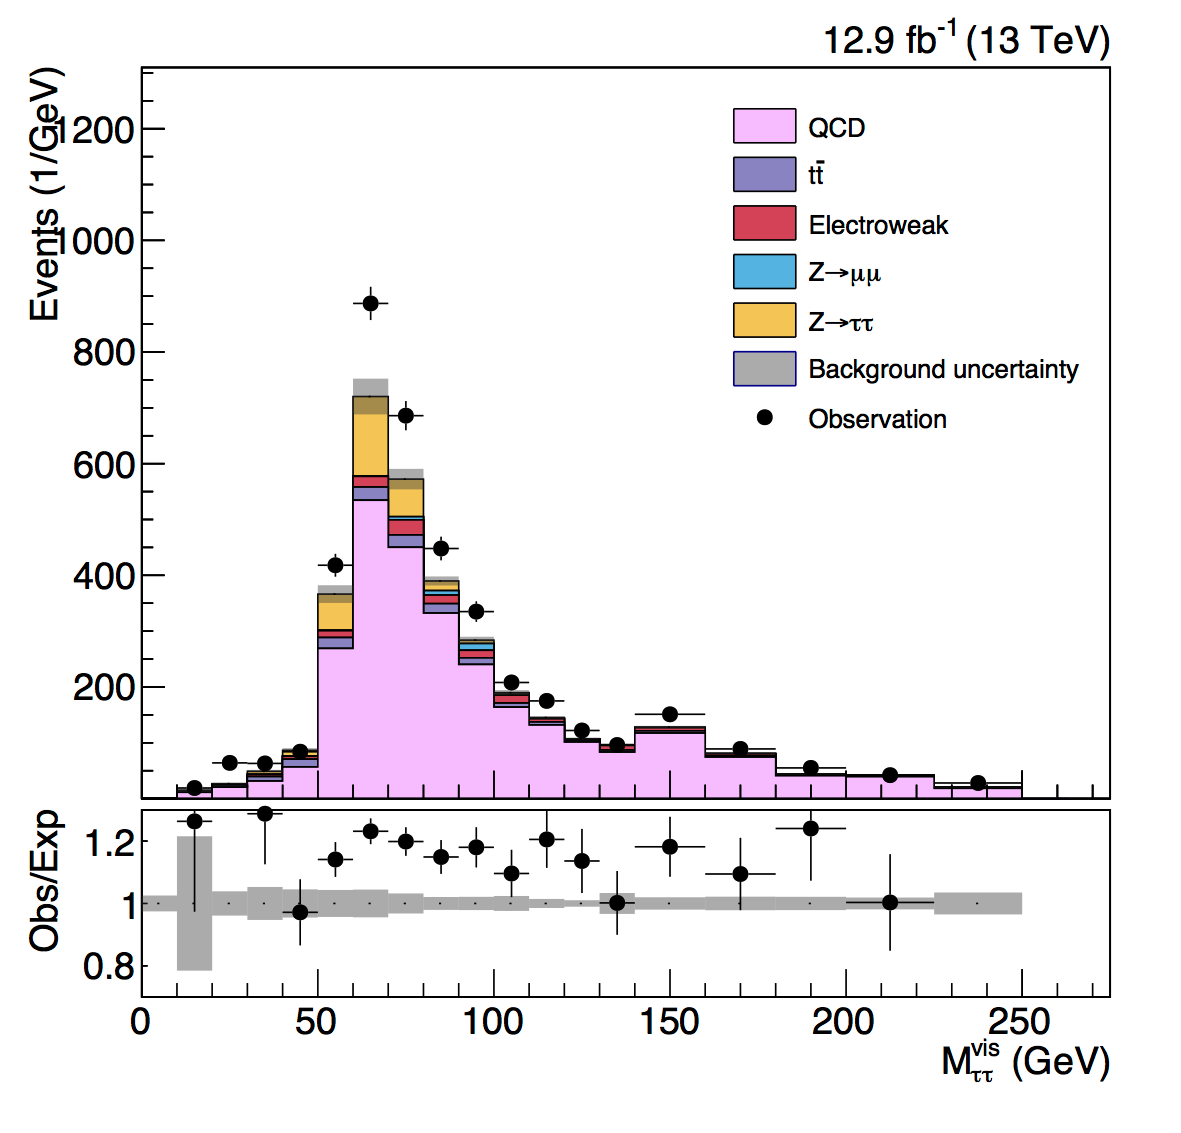
\includegraphics[width=0.5\textwidth]{./MSSM/Figures/qcdosss_far_mt_1_prefit.png}}
\subfloat[Post-fit distribution]{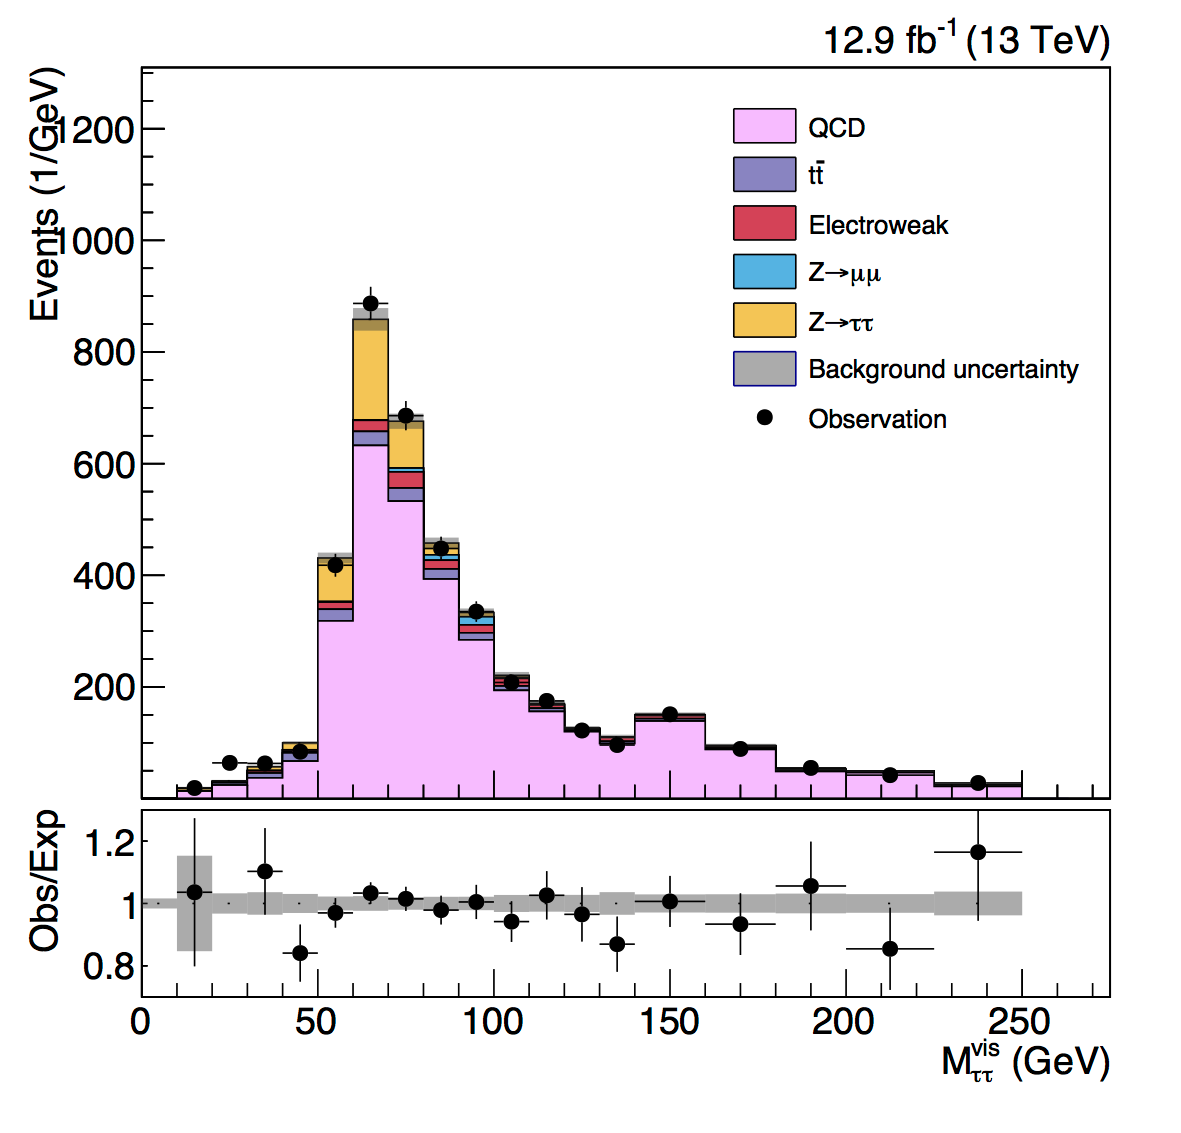
\includegraphics[width=0.5\textwidth]{./MSSM/Figures/qcdosss_far_mt_1_postfit.png}}
\end{center}
\caption[The visible mass distribution of the di-$\tau$ pair in the
\mutau channel for the sideband further away from the signal region,
before and after the maximum likelihood fit to the QCD signal strength.]{The visible mass distribution of the di-$\tau$ pair in the \mutau channel for the sideband further away from the signal region, (a) before
the maximum likelihood fit to the QCD signal strength and (b) after the fit. The resulting fitted signal strength 
is 1.184$\pm$0.035.}
\label{fig:mssm_qcdosss_mtfar}
\end{figure}

\begin{figure}[h!]
\begin{center}
\subfloat[Pre-fit distribution]{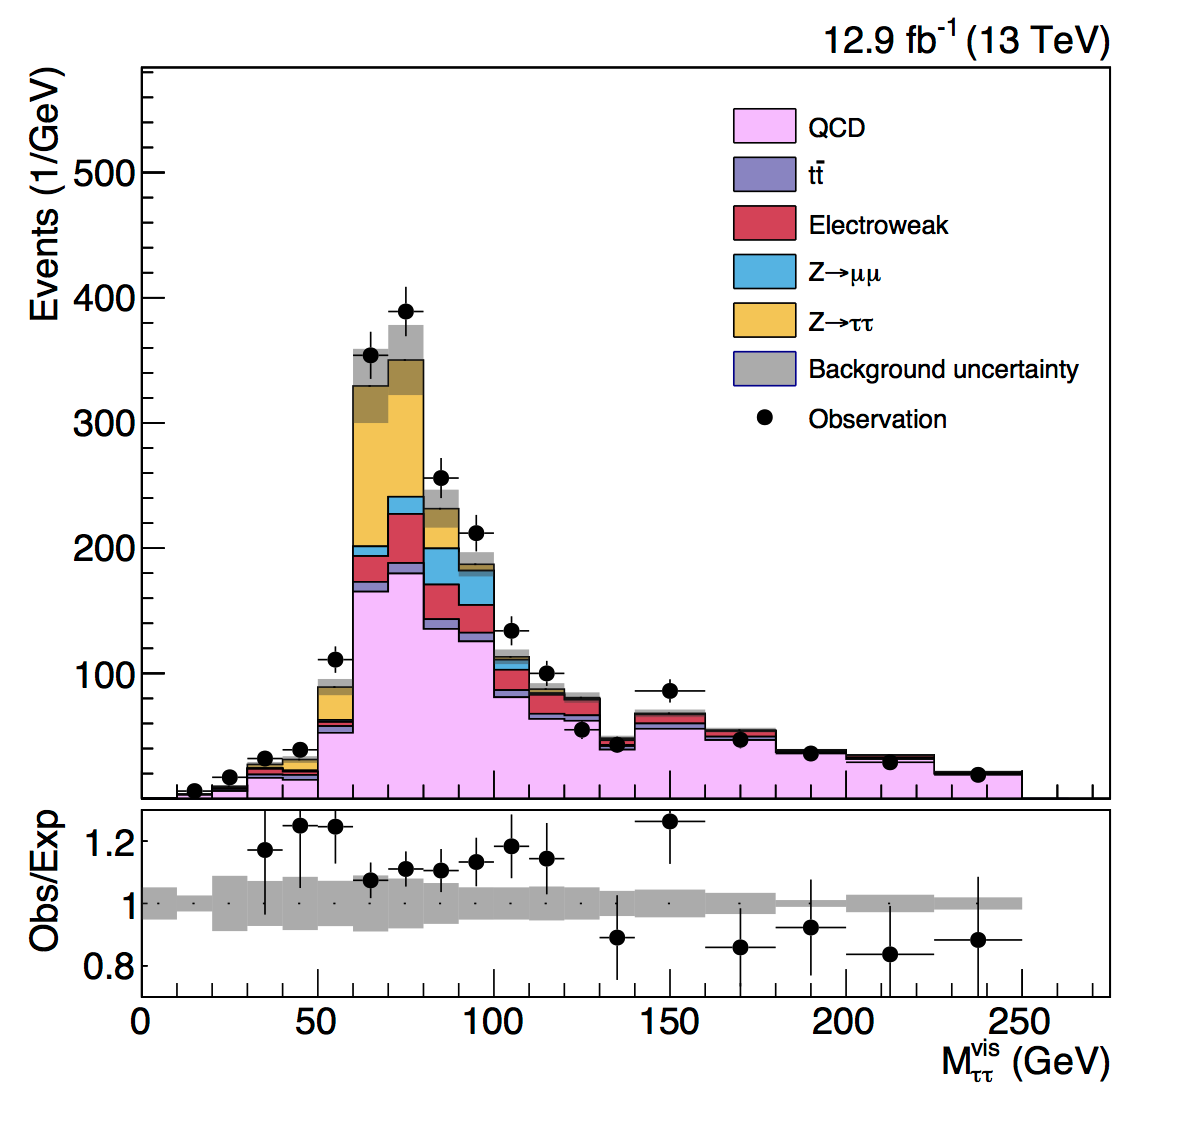
\includegraphics[width=0.5\textwidth]{./MSSM/Figures/qcdosss_near_et_1_prefit.png}}
\subfloat[Post-fit distribution]{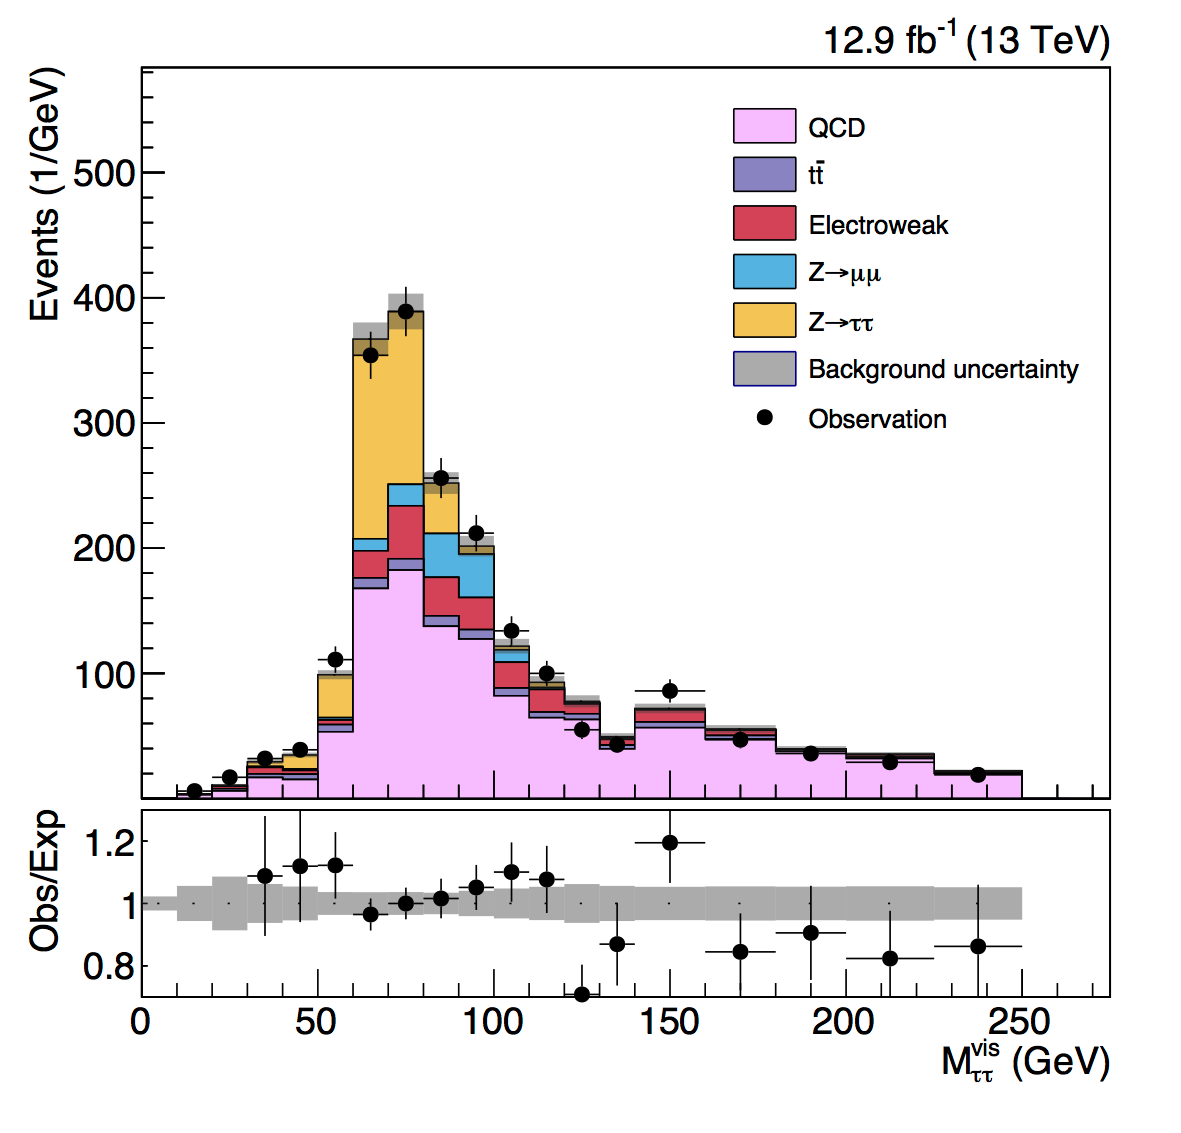
\includegraphics[width=0.5\textwidth]{./MSSM/Figures/qcdosss_near_et_1_postfit.png}}
\end{center}
\caption[The visible mass distribution of the di-$\tau$ pair in
the \etau channel for the sideband near the signal region,
before and after the maximum likelihood fit to the QCD signal strength.]{The visible mass distribution of the di-$\tau$ pair in the \etau channel for the sideband near the signal region, (a) before
the maximum likelihood fit to the QCD signal strength and (b) after the fit. The resulting fitted signal strength is 1.015$\pm$0.059.}
\label{fig:mssm_qcdosss_etnear}
\end{figure}

\begin{figure}[h!]
\begin{center}
\subfloat[Pre-fit distribution]{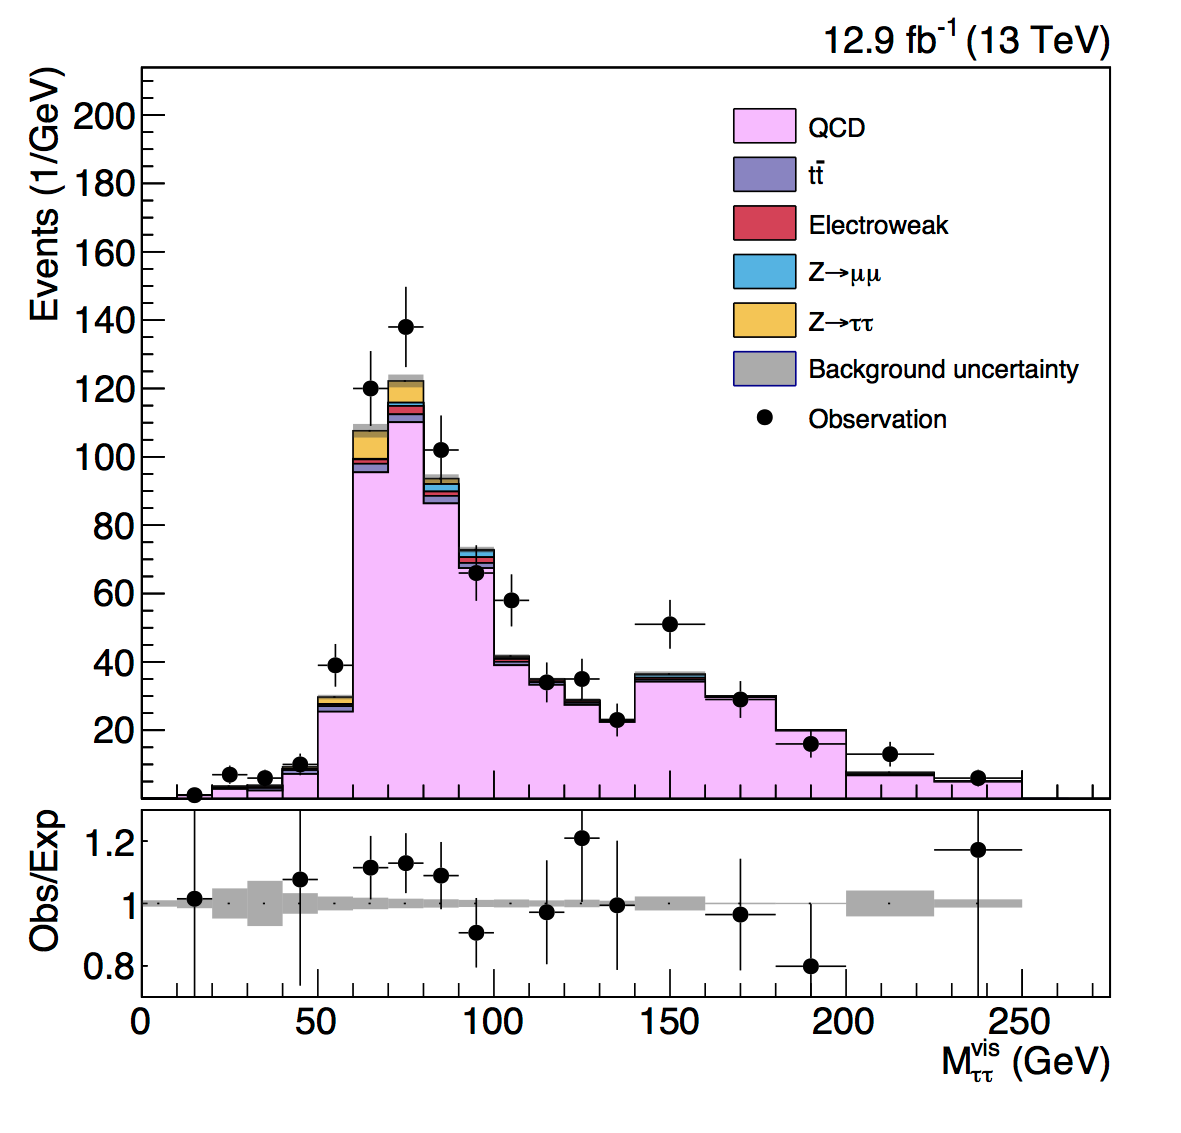
\includegraphics[width=0.5\textwidth]{./MSSM/Figures/qcdosss_far_et_1_prefit.png}}
\subfloat[Post-fit distribution]{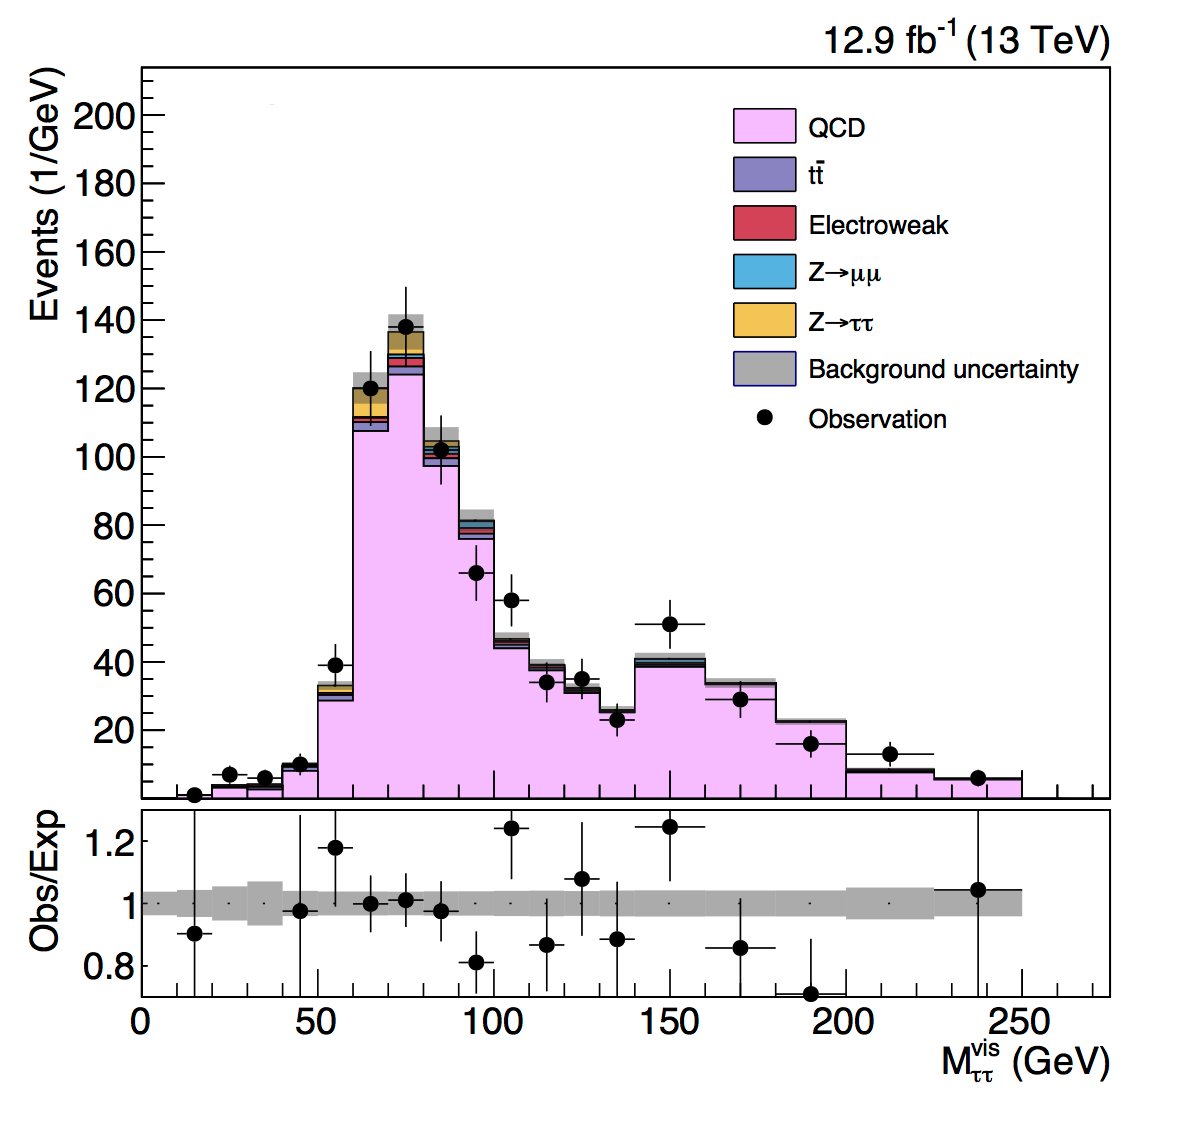
\includegraphics[width=0.5\textwidth]{./MSSM/Figures/qcdosss_far_et_1_postfit.png}}
\end{center}
\caption[The visible mass distribution of the di-$\tau$ pair
in the \etau channel for the sideband further away from the signal
region, before and after the maximum likelihood fit to the QCD signal 
strength.]{The visible mass distribution of the di-$\tau$ pair in the \etau channel for the sideband further away from the signal region, (a) before
the maximum likelihood fit to the QCD signal strenght and (b) after the fit. The resulting fitted signal strength
is 1.127$\pm$0.045.}
\label{fig:mssm_qcdosss_etfar}
\end{figure}

\subsubsection{QCD normalisation}
\label{sec:mssm_bkgs_etmt_qcdnorm}
The QCD normalisation is estimated by inverting the opposite-sign requirement
of the di-tau pair in the signal region. The yield is taken from the same--sign
region with otherwise identical cuts to the opposite--sign region. The contributions
from other backgrounds in this region are subtracted to give an estimate of the number
of QCD events in the same--sign region. For all backgrounds apart from \Wjets the
yields to subtract are estimated using \ac{MC} samples. The number of \Wjets events
expected in this region is given by
\begin{equation}\label{eqn:wjets_qcdsub}
N_{\text{W,SS low }m_{\text{T}}} = \frac{N_{\text{MC,SS low }m_{\text{T}}}}{N_{\text{MC,SS high }m_{\text{T}}}}N_{\text{W,SS high }m_{\text{T}}}.
\end{equation}
Because opposite--sign and same--sign QCD events do not
necessarily appear in equal amounts the number of QCD
events obtained by subtracting other backgrounds from the
observed number of events in the same--sign region is multiplied
by $R_{\text{QCD}}^{\text{OS/SS}}$ as derived in section \ref{sec:mssm_bkgs_etmt_qcdosss} 
to obtain an estimate of the number of QCD events in the signal region.
%\subsubsection{Control regions in the fit}
%\label{sec:mssm_bkgs_etmt_ctrl}
%Several control regions in data are used for the estimation
%of the QCD and \Wjets backgrounds: the same--sign and 
%opposite--sign high \mT~regions, as well as the same--sign
%low \mT~region. This leads to three control regions used 
%in each category of both the \mutau and \etau channels to determine
%the initial estimate of the background normalisations.
%These control regions are included in a simultaneous fit
%with the signal regions to obtain the final results. More detail
%can be found in section \ref{sec:mssm_sigext_ctrl}.

\subsection{\texorpdfstring{QCD in the \tautau and \emu channels}{QCD in the tautau and emu channels}}
\label{sec:mssm_bkgs_qcd}
This section describes the QCD background
estimation in the \tautau and \emu channels, which takes a slightly
different form than in the \mutau and \etau channels.

\subsubsection{\texorpdfstring{\tautau channel}{tau tau channel}}
\label{sec:mssm_bkgs_qcd_tt}
In the \tautau channel QCD events constitute by far the dominant background.
The normalisation and shape 
of this background are estimated from a sideband with loosened 
isolation requirements with respect to the signal region. 
In the no b-tag category the sideband used is determined
by having the tau with highest \pT~pass the tight working
point of the tau ID discriminator, as in the nominal selection.
The other hadronic tau in the pair is required to fail the tight working point,
but pass the medium working point. This sideband is 
chosen as it is as close to the signal region as possible, and 
this should minimise biases in the shape of the total transverse mass
distribution. Other backgrounds
in this sideband are subtracted from the observation to give
the QCD estimate. Differences in normalisation due to
the use of a loosened sideband are corrected for by the medium-to-tight isolation
scale factor. This correction factor is measured as
\begin{equation}\label{eqn:tautau_qcd}
R_{QCD}^{\text{medium}\rightarrow\text{tight}} = \frac{N_{\text{data}}^{SS,\text{nominal isolation}}-N_{\text{other bkgs}}^{SS,\text{loosened isolation}}}{N_{\text{data}}^{SS,\text{loosened isolation}}-N_{\text{other bkgs}}^{SS,\text{loosened isolation}}}.
\end{equation}
This correction factor takes the ratio between the observed data with other
backgrounds subtracted in the region equivalent to the signal region, but with the
charge requirement of the pair inverted, and the region equivalent to the sideband
with loosened isolation but with the charge requirement on the pair inverted.

The QCD estimate in the b-tag category is derived using an analogous method, 
 however, the sideband as used for the 
no b-tag category does not contain enough events to 
provide a background estimate. Therefore a sideband where
the highest \pT~tau passes the tight working point of the
tau ID discriminator, and the other tau passes the loose working
point of the discriminator, but not the tight working point, is used.
This sideband is slightly further away from the signal region than the
`tight--medium' sideband. %The bias from using this looser
%sideband has been assessed and has a less than 1$\sigma$ effect.
%FIXME THIS ISN'T VERY USEFUL INFO!

\subsubsection{\texorpdfstring{\emu channel}{e mu channel}}
\label{sec:mssm_bkgs_qcd_em}
In the \emu channel the QCD background
is estimated by inverting the charge requirement
of the pair, considering the same--sign region
with otherwise identical cuts to the signal region.
Other backgrounds present in this region are subtracted.
Like for the \etau and \mutau channels, the number of
QCD events with opposite--sign \emu pairs is not
necessarily equal to the number of QCD events
with same--sign \emu pairs and therefore the ratio
of opposite--sign to same--sign pairs is measured by inverting
the isolation requirements on the electron or muon. Both
leptons need to satisfy $I_{\text{rel}} < 0.4$ and at 
least one of them needs to fail the nominal isolation requirement.
The opposite--sign to same--sign ratio is parameterised in terms
of lepton kinematics and the separation in $\Delta R$ between the
two leptons. These ratios are then applied to the estimate in the same--sign region
to give an estimate in the signal region. The statistical uncertainty
on the measurement is 13\%. Cross-checking the measurement 
using QCD \ac{MC} samples, it is observed that there is a 19\% difference
between the OS/SS ratio in the signal region and the sideband, the two
uncertainties are added in quadrature. 
The opposite--sign to same--sign ratios are measured
before applying the categorisation, and because \ac{MC} studies suggest
that the opposite--sign to same--sign ratio is different in the b-tag
category than in the no b-tag category, an extra scale factor of 
1.45/2.20 $\pm$ 0.16 is applied to the QCD estimate in the b-tag category. This is 
the ratio between the OS/SS ratio as measured in the b-tag category and 
the measurement made before categorisation. The uncertainty is added in
quadrature to the statistical and systematic uncertainties already described.


\subsection{\texorpdfstring{\ttbar}{ttbar}}
\label{sec:mssm_bkgs_tt}
The \ttbar shape and normalisation are estimated from \ac{MC} 
samples and are checked against data in a control
region with a \ttbar purity of 91\%. This control region
is defined as $D_{\zeta} < -20$ GeV and \MET $>80$ GeV in 
the \emu channel, and it is shown in figure \ref{fig:mssm_corrs_toppt}b.
Because the 6\%
\ttbar normalisation uncertainty covers the observed
discrepancy between data and \ac{MC}, no scale factor is applied.
In the \mutau, \etau and \tautau channels
the \ttbar contribution is split into
two components, one with real taus and 
one without, for fitting purposes. The component with real taus is composed
of \ttbar events in which the hadronic tau is matched
to a generator level tau. In the fully hadronic channel
both taus need to be generator matched to a hadronically
decaying tau.



\subsection{Other backgrounds}
\label{sec:mssm_bkgs_other}
For all channels the di--boson plus 
single--top background is small.
Both normalisation and shape are estimated from \ac{MC}
samples. For the \etau, \mutau and \tautau channels
this background contribution is split into a component
where the hadronically decaying tau originates from a real
tau, and one where it does not, for purposes of the fit. This is done in a similar
way as for the \ttbar background.
In the \tautau and \emu channels the \Wjets background
is less important than in the \etau and \mutau channels, and both
its shape and normalisation are estimated from the
\ac{MC} samples. In the \emu channel the $\PW\Pphoton$ background
is also added to the \Wjets background component. For plotting purposes the single-top plus
di-boson and \Wjets backgrounds are drawn together as the `electroweak' contribution for all channels, even though
they are considered as separate components in the fit.


\section{Systematic uncertainties}
\label{sec:mssm_uncs}
As for the analysis presented in chapter \ref{chap:hhh}
two types of systematic uncertainty are considered. Normalisation
uncertainties only affect the yield of a process while shape
uncertainties affect both the process normalisation and the shape
of the \mTtot~distribution. The uncertainties are taken into account 
in the final result as described in section \ref{sec:hhh_results_extraction}.

\subsection{Normalisation uncertainties}
\label{sec:mssm_uncs_norm}
\subsubsection*{Luminosity uncertainty}
The uncertainty on the luminosity measurement amounts to 6.2\% for
data collected during 2016 \cite{cms-pas-lum-15-001}, and it is
applied to all processes for which the normalisation is estimated 
using \ac{MC} samples.
\subsubsection*{Identification, isolation and trigger efficiencies}
The combined uncertainty on the electron and muon identification, isolation, and
trigger efficiencies amounts to 2\% \cite{CMS-PAS-HIG-16-037}. For hadronic taus the identification and
isolation uncertainty amounts to 6\% in the \etau and \mutau channels
and 12\% in the \tautau channel, with an additional 7\% uncertainty
on the tau trigger efficiency added in quadrature for that channel \cite{CMS-PAS-HIG-16-037}. This
uncertainty is split between a part that is correlated between the channels, 
a 5\% (10\%) uncertainty in the \etau and \mutau (\tautau) channels. The uncorrelated 
part amounts to 3\% (9.2\%) for the \etau and \mutau (\tautau) channels.
The uncertainties on lepton/hadronic tau identificiation, isolation and 
trigger efficiency are applied to all processes for which the normalisation
is estimated using \ac{MC} samples.
\subsubsection*{jet$\rightarrow\Pgt_{h}$ fake rate}
The uncertainty on the jet$\rightarrow\Pgt_{h}$ fake rate
is 20\% \cite{cms-tau-2015}. This uncertainty is applied
to those backgrounds where the normalisation is estimated from \ac{MC} and
where the hadronic taus are mimicked by jets, that is the \Zellell background
with a jet faking a hadronic tau, the \Wjets background in the fully hadronic
channel, and the \ttbar background without real hadronic taus.
\subsubsection*{$\Pe\rightarrow\Pgt_{h}$ and $\Pgm\rightarrow\Pgt_{h}$ fake rate}
The $\Pe\rightarrow\Pgt_{h}$ fake rate uncertainty ranges from 10-30\%,
depending on the anti-electron discriminator used \cite{cms-tau-2015}. This uncertainty is 
applied to the \Zellell background with the hadronic tau faked by an electron.
The $\Pgm\rightarrow\Pgt_{h}$ fake rate uncertainty ranges from 20-30\%, depending
on the anti-muon discriminator used\cite{CMS-PAS-HIG-16-037}. This uncertainty is applied to the \Zellell
background with the hadronic tau faked by a muon.
\subsubsection*{Jet energy scale uncertainty}
The uncertainties on the jet-energy corrections are applied
by shifting the jet energy up and down by the \pT-and $\eta$-dependendent
uncertainty, and evaluating the change in the process normalisation in
each category. Where the change in normalisation is non-negligible the
uncertainty is applied. It ranges from 1--10\% depending on process and category.
\subsubsection*{B-tag scale factors}
Uncertainties on the b-tagging efficiency and light jet mis-tagging
rates are given as a function of jet \pT-and $\eta$-for the 
medium working point of the \ac{CSV}v2 discriminator \cite{cms-btag-run2}.
The b-tagging scale factors are are varied within these uncertainties
and the overall change in normalisation for each process in each category is
evaluated. If the change in normalisation is non-negligible this
uncertainty is applied. The uncertainty varies from 1--5\%.
\subsubsection*{\MET~resolution and response}
Uncertainties on the \MET~resolution and response are estimated
by varying the recoil correction parameters within their
uncertainty and evaluating the effect on process
normalisations. The uncertainty amounts to around 2\%.
\subsubsection*{Background normalisation uncertainties}
\begin{itemize}
\setlength{\itemsep}{-\baselineskip}
\item \Ztautau: As the \Zmm control region is included in the simultaneous
fit with the signal region to correct the \Ztautau normalisation,
the Drell-Yan cross section is not applied as an uncertainty. In the no b-tag (b-tag) category a 3\% (5\%)
extrapolation uncertainty from \Zmm to \Ztautau is applied \cite{CMS-PAS-HIG-16-037}.
\item \Zellell: The uncertainty on the Drell-Yan cross-section
is to 4\% \cite{CMS-PAS-HIG-16-037}.
\item \ttbar: The uncertainty on the \ttbar production cross-section amounts
to 6\% \cite{CMS-PAS-HIG-16-037}.
\item di-boson and single-top: The uncertainty on the di-boson and
single-top production cross-sections amounts to 5\% \cite{CMS-PAS-HIG-16-037}.
\item \Wjets: In the \mutau and \etau channels the statistical uncertainties
on the observed data and subtracted backgrounds in the control regions are taken into account by
the inclusion of these control regions in the fit. The statistical
uncertainty on $R_{W}^{\text{OS/SS}}$ amounts to 2\% in the no b-tag
category in both the \etau and \mutau channels, and 11\% (14\%) in the b-tag
category of the \mutau (\etau) channel. The systematic uncertainty on
this ratio amounts to 8\% (10\%) in the no b-tag (b-tag) category of both channels.
The statistical uncertainty on the low \mT/high \mT~ratio is 2\% in the no b-tag
category of both channels and 14\% (17\%) in the b-tag category of the \mutau (\etau) channel.
The systematic uncertainty on this ratio amounts to 20\%. As the \Wjets background
in the \tautau and \emu channels is estimated from \ac{MC} a 4\% theoretical
production cross-section uncertainty is applied.
\item QCD: In the \emu channel the uncertainty on the QCD estimate
is taken as the uncertainty on the measured opposite--sign to same--sign
ratio, which is 23\% in the no b-tag category and 34 \% in the b-tag category. In the
\tautau channel the statistical uncertainty on the QCD estimate is derived from
the uncertainties on the observations and subtracted backgrounds in the
sidebands used to derive the estimate. This uncertainty amounts to 3\% in the no b-tag
category and 20\% in the b-tag category. An additional systematic uncertainty on the
extrapolation factor from the anti-isolated sideband into the signal region is found
to be 12\% in the no b-tag category and 14 \% in the b-tag category. For the \etau and
\mutau channels the statistical
uncertainties on the observation and subtracted \ac{MC} backgrounds in the control
region used to derive the QCD estimate is accounted for by the inclusion of these control
regions in the fit. The uncertainty on the opposite--sign to same--sign ratio, based on
the studies described in section \ref{sec:mssm_bkgs_etmt_qcdosss} is found to be 4\% (60\%) in the 
no b-tag (b-tag) category of the \mutau channel, and 12\% (60\%) in the no b-tag (b-tag) category
of the \etau channel. 
\end{itemize}
\subsubsection*{Signal theory uncertainties}
For interpretations of the results in MSSM benchmark scenarios, theory
uncertainties on the SM and MSSM Higgs cross--section predictions are taken into account.
The uncertainties for the SM signal processes are described in more detail in reference \cite{YR4}.
Uncertainties due to different renormalisation scales
amount to 3.9\% for gluon fusion,
0.4\% for VBF, 2.8\% for ZH and 0.5\% for WH. The uncertainties
due to different choices of pdf set and $\alpha_s$ amount to 3.2\% for gluon fusion, 2.1\% for vector boson fusion,
1.6\% for ZH and 1.9\% for WH.
For the MSSM Higgs cross--sections used in the models, the uncertainties
due to different choices of factorisation and renormalisation scale
are computed, separately for each \mA-\tanb~point, following the prescription in Refs. \cite{pdf-lhc,alphas-uncs}.

\subsection{Shape uncertainties}
\label{sec:mssm_uncs_shape}
\subsubsection*{$\Pgt_{h}$ energy scale}
The energy of hadronic taus is varied up and down by 3\% \cite{CMS-PAS-HIG-16-037}, affecting
the shape of the total transverse mass distribution.
The uncertainty is applied to the signal samples and to
backgrounds containing real hadronic taus in the \etau, \mutau, and \tautau channels, namely
\Ztautau, and the components of the \ttbar and single-top+di-boson background with real 
hadronic taus.
\subsubsection*{Electron energy scale}
The energy of electrons is varied by 1\% in the barrel and by 2.5\% in the endcaps \cite{CMS-PAS-HIG-16-037}. This 
uncertainty is applied to the
signals and to the \Ztautau background in the \emu channel.
\subsubsection*{High-\pT~$\Pgt_{h}$ ID efficiency}
An additional $\Pgt_{h}$ identification uncertainty of $\frac{20\% \times p_{\text{T}}}{\text{TeV}}$
is applied to account for the extrapolation from the tau ID efficiency
measurement, which uses mostly taus close to the Z peak, to taus with higher transverse momenta \cite{CMS-PAS-HIG-16-037}. This
uncertainty is applied to signal and backgrounds with real taus in the \etau, \mutau and \tautau channels.
The shape difference between the nominal, up- and down- shapes for this uncertainty in the no b-tag category
of the \tautau channel can be seen for a high-mass signal sample in figure \ref{fig:mssm_highpttauid_shapes}a and
for the \Ztautau background in figure \ref{fig:mssm_highpttauid_shapes}b. Because the \Ztautau background
has much softer hadronic taus than the high-mass signal sample, the impact of this uncertainty on the shape
is much smaller.
\begin{figure}[h!]
\begin{center}
\subfloat[gg$\phi$ signal at $m_{\phi} = 3.2$ TeV]{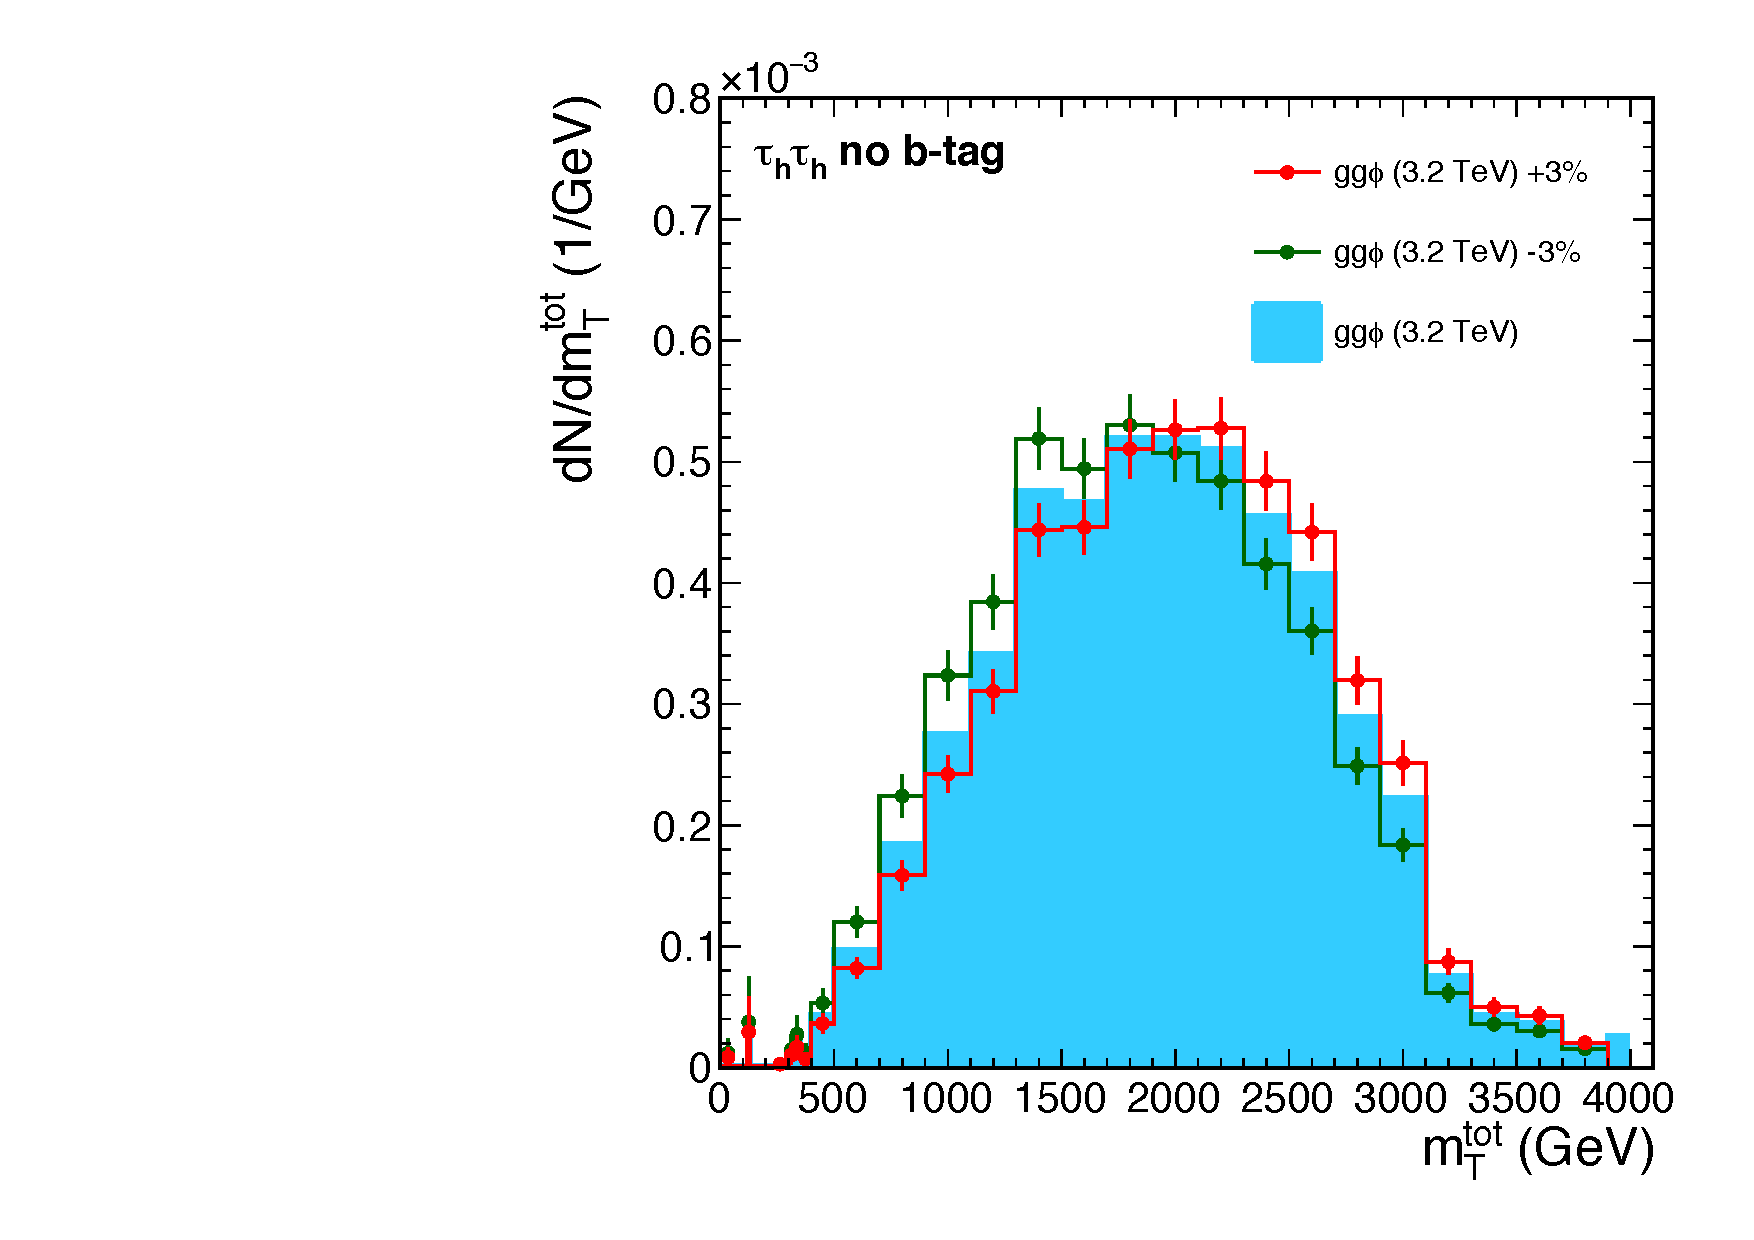
\includegraphics[width=0.5\textwidth]{./MSSM/Figures/highpT_tauID_comp_tt_nobtag_ggh3200.pdf}}
\subfloat[\Ztautau background]{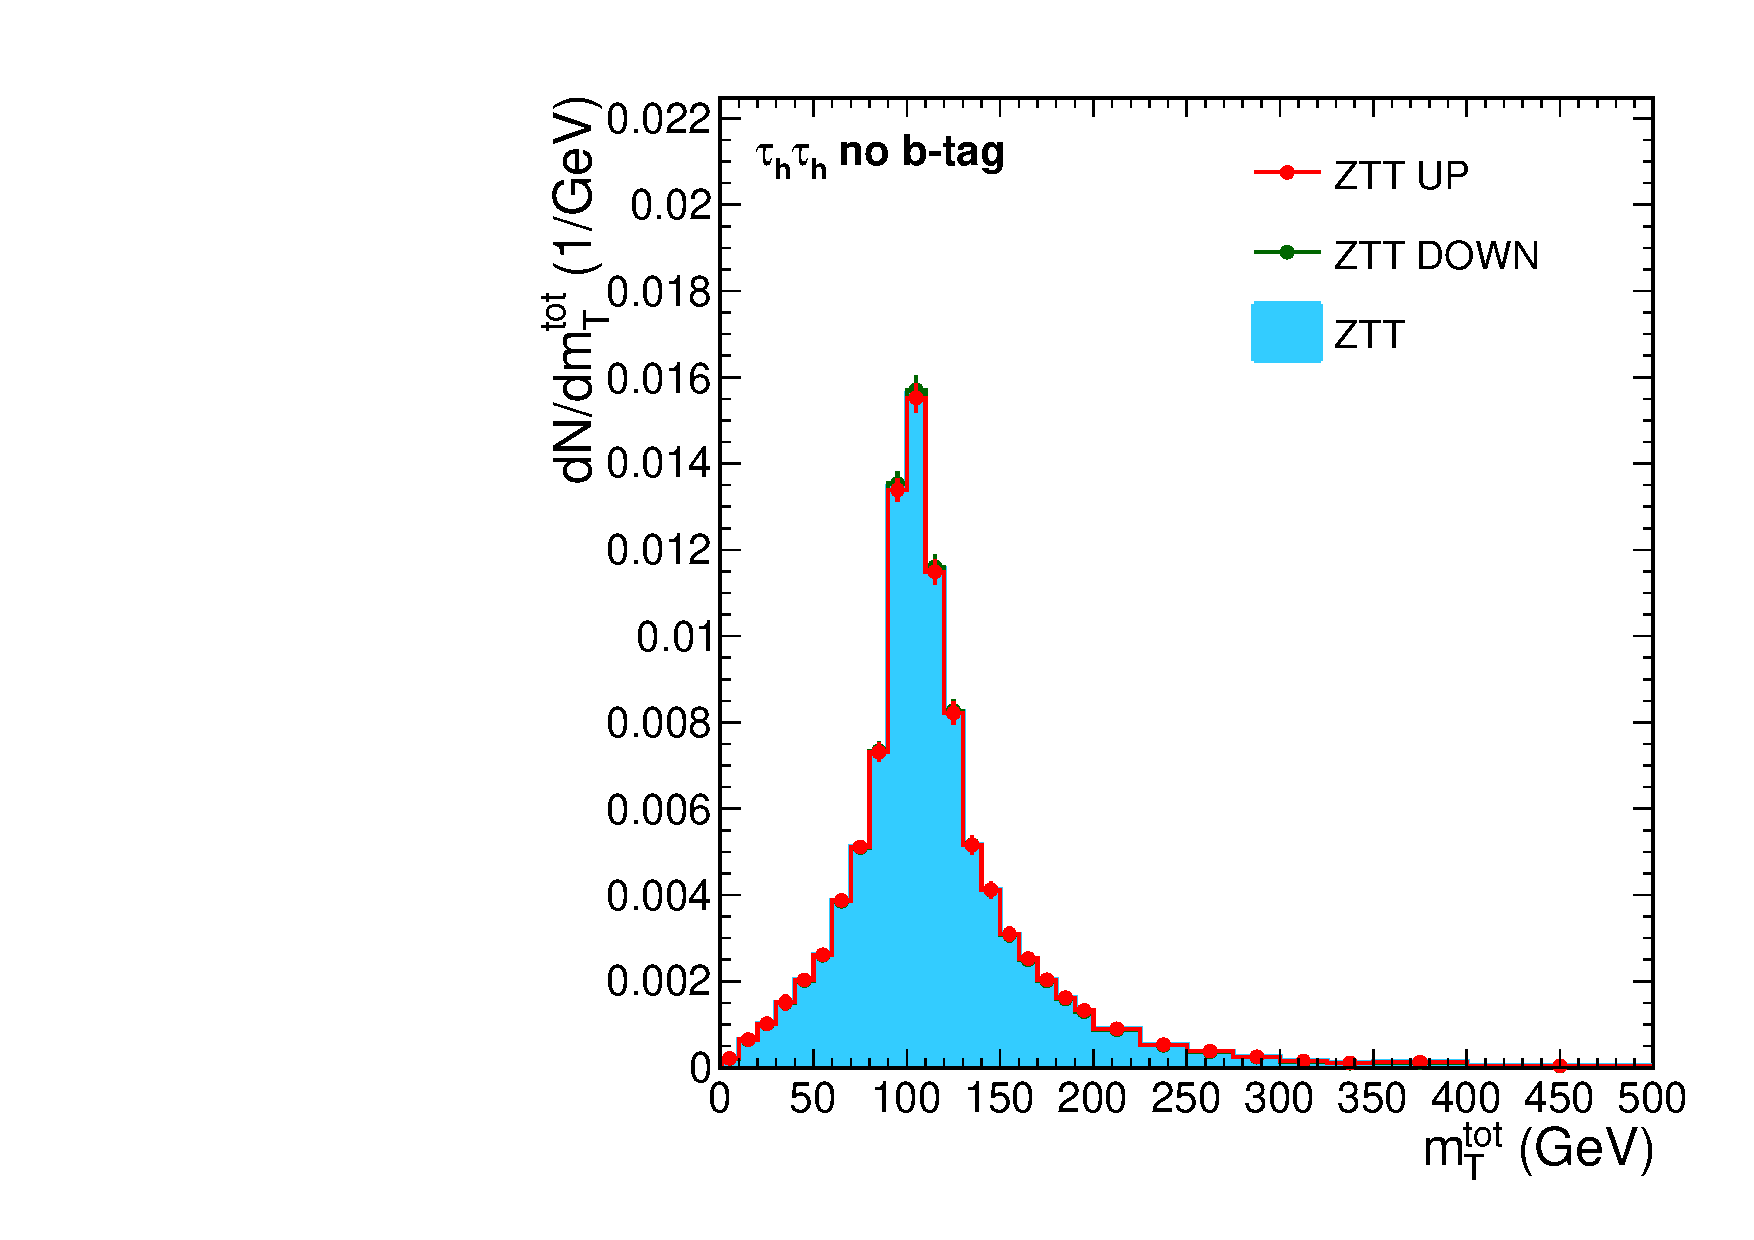
\includegraphics[width=0.5\textwidth]{./MSSM/Figures/highpT_tauID_comp_tt_nobtag_ZTT.pdf}}
\end{center}
\caption[Impact of the high-\pT~tau ID uncertainty in the no b-tag category
of the \tautau channel for a high-mass signal sample and the \Ztautau
background.]{Impact of the high-\pT~tau ID uncertainty in the no b-tag category of the
\tautau channel for (a) a high-mass signal sample and (b) the \Ztautau background. The effect on the shape is much
larger in the high-mass signal sample, which contains hadronically decaying taus with much higher
\pT~than the \Ztautau sample.}
\label{fig:mssm_highpttauid_shapes}
\end{figure}
\subsubsection*{Top quark \pT~reweighting}
To account for the uncertainty in the derivation of the top-quark \pT~reweighting, a shape
uncertainty is applied to the \ttbar background. This uncertainty amounts to a 100\% variation
of the correction, that is the difference between applying the correction twice and not applying the correction at all.
\subsubsection*{Drell-Yan shape reweighting}
An uncertainty on the Drell-Yan shape reweighting based on \Zmm events
is applied as 100\% of the correction to the \Ztautau background \cite{CMS-PAS-HIG-16-037}. 
\subsubsection*{Jet$\rightarrow\Pgt_{h}$ fake rate shape reweighting}
On the \Wjets background in the \etau and \mutau channels a shape 
uncertainty of $\frac{-20\% \times p_{\text{T}}}{\text{GeV}}$ is 
applied. This uncertainty is derived from variations in the data/MC ratio
for the jet$\rightarrow\Pgt_{h}$ fake rate as a function of jet \pT~in 
\Wjets events \cite{CMS-PAS-HIG-16-037}.

Overview tables of the systematic uncertainties per category of each
channel can be found in appendix \ref{appendix:uncerts}. The correlations
between the different channels and categories for these uncertainties
is also indicated.

\section{Signal extraction}
\label{sec:mssm_signalextraction}
The total transverse mass \mTtot~is used as discriminating variable in this analysis.
All bins of the distribution are used to perform a shape analysis. The general statistical
methods, including the incorporation of nuisance parameters in the fit, were 
described in section \ref{sec:hhh_results_extraction}. Some additional
methods are used for this analysis, and they will be discussed in this section.

\subsection{Inclusion of control regions in the fit}
\label{sec:mssm_sigext_ctrl}
The control regions used for estimation of the 
\Wjets and QCD background contributions in the signal regions, discussed
in section \ref{sec:mssm_bkgs_etmt_ctrl}, are included in the fit. They
are added to the likelihood as single-bin counting experiments. In a given
category of one of the channels, the \Wjets
normalisation is fully correlated between the three control 
regions and the signal region. One common, freely floating, nuisance parameter
controls the \Wjets normalisation in all four regions. The QCD normalisation
is fully correlated between the opposite--sign and same--sign low-\mT~regions. The
same is true for the opposite--sign and same--sign high-\mT~regions. This means there are
two freely floating nuisance parameters that govern the QCD normalisation: one
that controls the QCD normalisation in the two low-\mT~regions, and one
that controls it in the two high-\mT~regions.

The \Zmm control regions mentioned in section \ref{sec:mssm_bkgs_ztt}
are also included in the likelihood as single-bin counting experiments.
The \Zmm control region in the no b-tag category is tied
to the \Ztautau normalisation in the no b-tag categories of all four
channels, again being controlled by a freely floating nuisance parameter. 
The same is true for the \Zmm control region in the b-tag category
and the \Ztautau normalisation in the b-tag categories of all four channels.

\subsection{Signal process profiling and 2D likelihood scans}
\label{sec:mssm_sigext_profile}
Because the analysis targets the two main MSSM production modes, gluon fusion and
b-associated production, limits are set on these two signal processes. As we
have seen in section \ref{sec:mssm_eventsel_categories}  we cannot fully separate the two signals by means
of the categorisation used. 
However, in the upper limits on cross--section times branching ratio for the gg$\phi$
process we should not make any assumptions about the presence or lack of the bb$\phi$
process and vice versa. Therefore when calculating the upper limits on the gg$\phi$ (bb$\phi$)
process, the contribution of the bb$\phi$ (gg$\phi$) process is profiled. This means it is floated
in the fit like a nuisance parameter.

Because the analysis targets these two signal processes, it is possible
to re-define the likelihood as a function of both the gg$\phi$ and bb$\phi$ signals:
\begin{equation}\label{mssm_2D_likelihood}
\mathcal{L}(\text{data}|\mu_{gg\phi},\mu_{bb\phi}, \theta) = \mathcal{L}(\text{data}|\mu_{gg\phi} \cdot s_{gg\phi}(\theta) + \mu_{bb\phi}\cdot s_{bb\phi}(\theta) + b(\theta)),
\end{equation}
where $s_{gg\phi}$ and $s_{bb\phi}$ are the signal expectations of the two
production processes and the signal strength modifiers $\mu_{gg\phi}$ and $\mu_{bb\phi}$ now represent the cross--section times branching ratio of the
two processes. Using this definition we can now perform a likelihood scan in two dimensions by 
constructing a two-dimensional grid in $\mu_{gg\phi}$ and $\mu_{bb\phi}$, both required to be greater than or equal to 0. 
The negative log-likelihood,
\begin{equation}\label{eqn:nll}
\text{NLL} = -\text{ln }\mathcal{L}(\text{data}|\mu_{gg\phi},\mu_{bb\phi},\theta),
\end{equation}
is then evaluated at each point. The point in the 2D grid where the NLL reaches
its lowest value gives the best fit value for $\mu_{gg\phi}$ and $\mu_{bb\phi}$.
68\% and 95\% confidence intervals are constructed as the values
$\mu_{gg\phi}^{N\%}$ and $\mu_{bb\phi}^{N\%}$ for which:
\begin{equation}\label{eqn:mssm_2D_deltaNLL}
\begin{split}
\Delta(\text{NLL})_{68\%} = \text{NLL}(\text{best fit}) - \text{NLL}(\mu_{gg\phi}^{68\%},\mu_{bb\phi}^{68\%}) = 0.5, ~\\
\Delta(\text{NLL})_{95\%} = \text{NLL}(\text{best fit}) - \text{NLL}(\mu_{gg\phi}^{95\%},\mu_{bb\phi}^{95\%}) = 1.92.
\end{split}
\end{equation}

\subsection{MSSMvsSM hypothesis testing}
\label{sec:mssm_sigext_mssmvssm}
The results of the search are interpreted in MSSM benchmark
scenarios, with the interpretation made in the \mA-\tanb~plane.
At each point in the \mA-\tanb~plane each MSSM scenario
predicts a production cross--section, and corresponding branching
ratio into $\Pgt\Pgt$, for each of the three neutral Higgs bosons. The
masses of the light h and the scalar H are also given as a function of \mA~and \tanb.
To interpret the results of this search in a particular scenario, the predicted
signal from the three neutral Higgs bosons is combined into a single signal template\footnote{Examples of what such a combined signal profile might look like are given in figures \ref{fig:mssm_results_mttot_mt}--\ref{fig:mssm_results_mttot_em},
which give the \mTtot~distributions for all channels and categories with an example three-Higgs signal overlaid.}.
In this way the compatibility of the data with all three Higgs bosons, not just a single one, is tested.

Simply comparing a three-Higgs-signal-plus-background hypothesis with a background-only 
hypothesis to determine the exclusion power of the search in a particular
model is not strictly correct. Due to the existence of a Higgs boson with a 
mass of 125 GeV, all MSSM benchmark scenarios must include a light Higgs boson
with very similar properties to the boson discovered during Run 1 of the \ac{LHC}.
Therefore we should perform a test that distinguishes between a three-Higgs-signal-plus-background hypothesis, and
a standard model Higgs-signal-plus-background hypothesis.

This means the likelihood function defined in equation \ref{eqn:hhh_likelihood}
must be modified. Instead of testing for the compatibility of the data with
a signal + background expectation modified by the signal strength modifier $\mu$ as
$\mu \cdot s(\theta) + b(\theta)$, a likelihood should be constructed as:
\begin{equation}\label{mssm_likelihood}
\mathcal{L}(\text{data}|\mu, \theta) = \mathcal{L}(\text{data}|\mu \cdot s_{\text{MSSM}}(\theta) + (1-\mu)\cdot s_{\text{SM}}(\theta) + b(\theta)),
\end{equation}
where $s_{\text{MSSM}}(\theta)$ corresponds to the MSSM signal expectation, that is the three-Higgs-signal, and $s_{\text{SM}}(\theta)$ 
corresponds to the SM signal expectation.
The signal strength modifier $\mu$ takes the role of distinguishing between
the two hypotheses in this case. The model must not allow for the coexistence 
of the SM and MSSM hypotheses; the MSSM hypothesis ($\mu=1$) has to be tested
against the SM hypothesis ($\mu=0$).

The modification of the likelihood function means it is no longer possible
to use the profile likelihood ratio of equation \ref{eqn:hhh_profilelikelihood}:
we need to test $\mu=1$ against $\mu=0$, and 
$\hat{\mu}$ in the denominator of equation \ref{eqn:hhh_profilelikelihood} is in 
general not 0. A solution to this problem can be found in the test statistic used at the Tevatron \cite{LHCHComb2011},
\begin{equation}\label{eqn:mssm_tevatron_teststat}
q_{\mu} = -2\text{ln }\frac{\mathcal{L}(\text{data}|\mu,\hat{\theta_{\mu}})}{\mathcal{L}(\text{data}|0,\hat{\theta_0})} \text{ with } 0\leq\mu.
\end{equation}
In this test statistic we test a positive value of $\mu$ against $\mu=0$, thus we are able to define
the desired `MSSMvsSM' test statistic, using $\mu=1$, as,
\begin{equation}\label{eqn:mssm_mssmvssm_stat}
q_{\text{MSSMvsSM}} = -2\text{ln }\frac{\mathcal{L}(\text{data}|s_{\text{MSSM}}(\theta) + b(\theta))}{\mathcal{L}(\text{data}|s_{\text{SM}}(\theta)+b(\theta))}.
\end{equation}

The asymptotic approximation, discussed in section \ref{sec:hhh_results_extraction}, can not be applied
to the Tevatron test statistic, and therefore the probability density functions need to be generated 
with toy datasets. Using these probability density functions  we can then calculate $CL_s(\mu=1)$ as defined in equation \ref{eqn:hhh_cls}.
If $CL_s < 0.05$ the MSSM hypothesis is excluded at 95\% CL. The generation of toy datasets and 
calculation of corresponding $CL_s$ values is performed for many points in a grid in the \mA-\tanb~plane,
with interpolation between grid points performed to obtain a smooth exclusion contour.
The pdfs for the SM and MSSM hypotheses, as well as the resulting $CL_s$ values,
are given for three illustrative \mA-\tanb~points in figure \ref{fig:mssm_mssmvssm_toys}. In figure \ref{fig:mssm_mssmvssm_toys}a
there is no separation between the MSSM and SM pdfs, and so we cannot exclude this point. The separation
between the pdfs in figure \ref{fig:mssm_mssmvssm_toys}b is much improved, and the observation is most compatible
with the SM hypothesis. This point is on the edge of being excluded. Finally the pdfs in figure \ref{fig:mssm_mssmvssm_toys}c
are very well separated, and the observation is compatible with the SM hypothesis, meaning this point of the parameter space is excluded.

\begin{figure}[h!]
\begin{center}
\subfloat[\mA=1.2 TeV, \tanb=16]{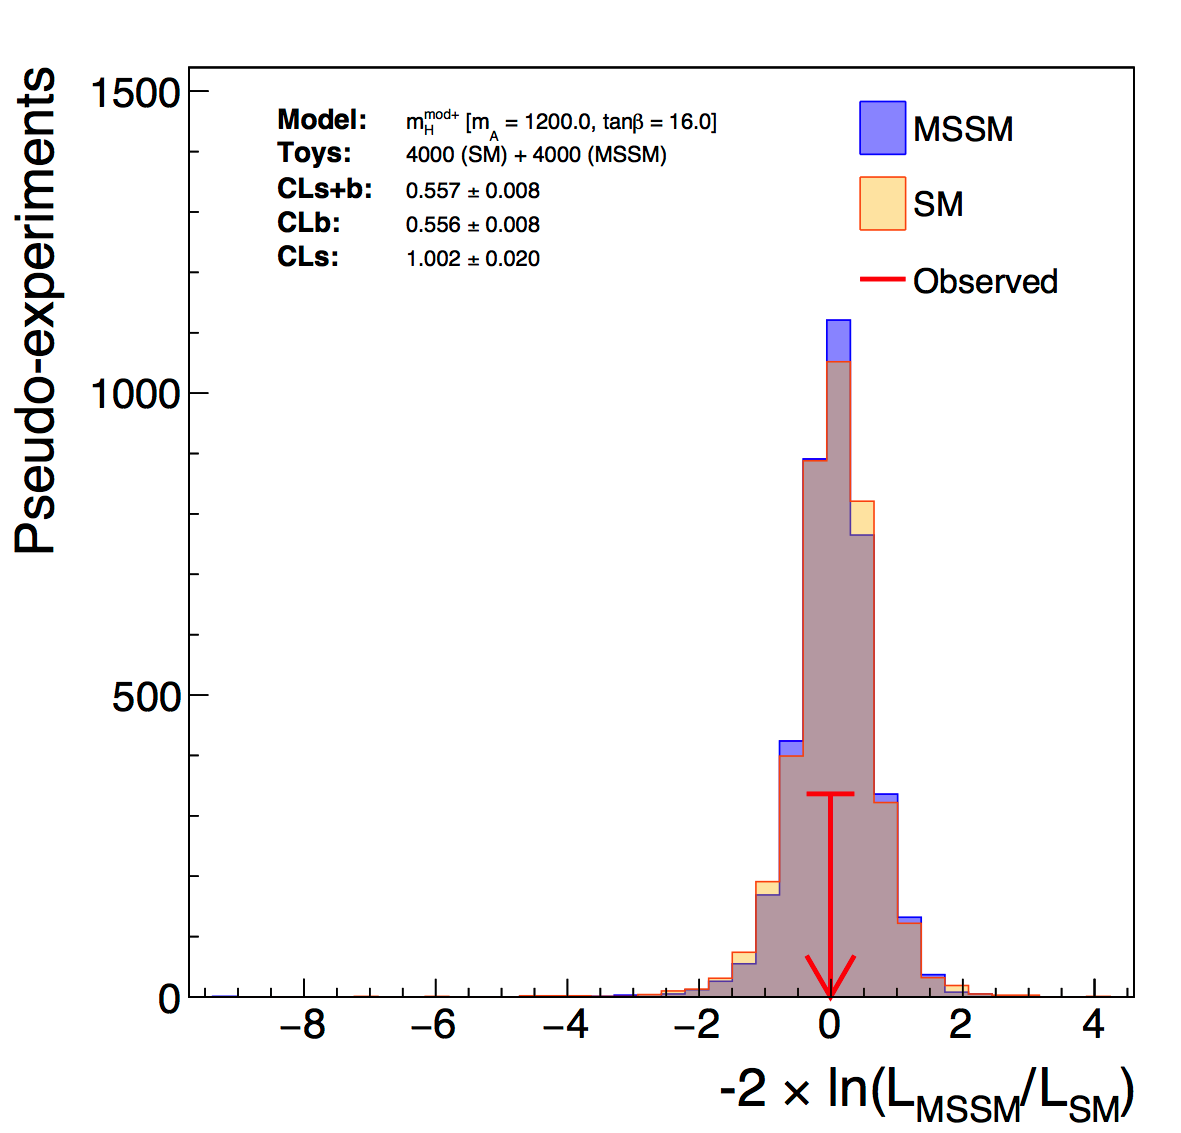
\includegraphics[width=0.5\textwidth]{./MSSM/Figures/plot_mA_1200_tanb_16.png}}
\subfloat[\mA=1.2 TeV, \tanb=50]{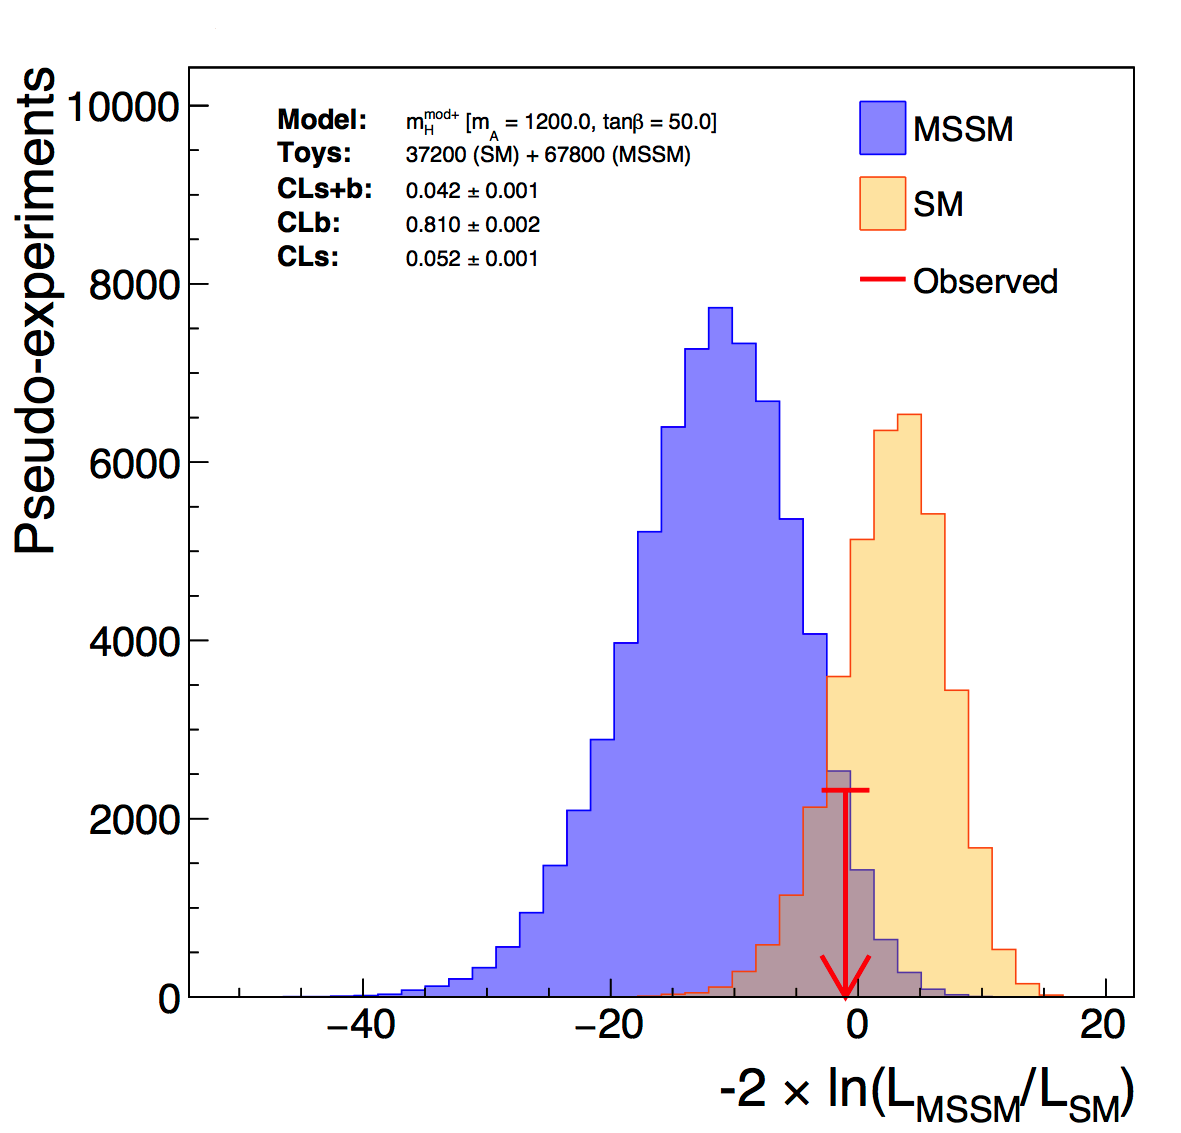
\includegraphics[width=0.5\textwidth]{./MSSM/Figures/plot_mA_1200_tanb_50.png}}~\\
\subfloat[\mA=700 GeV, \tanb=60]{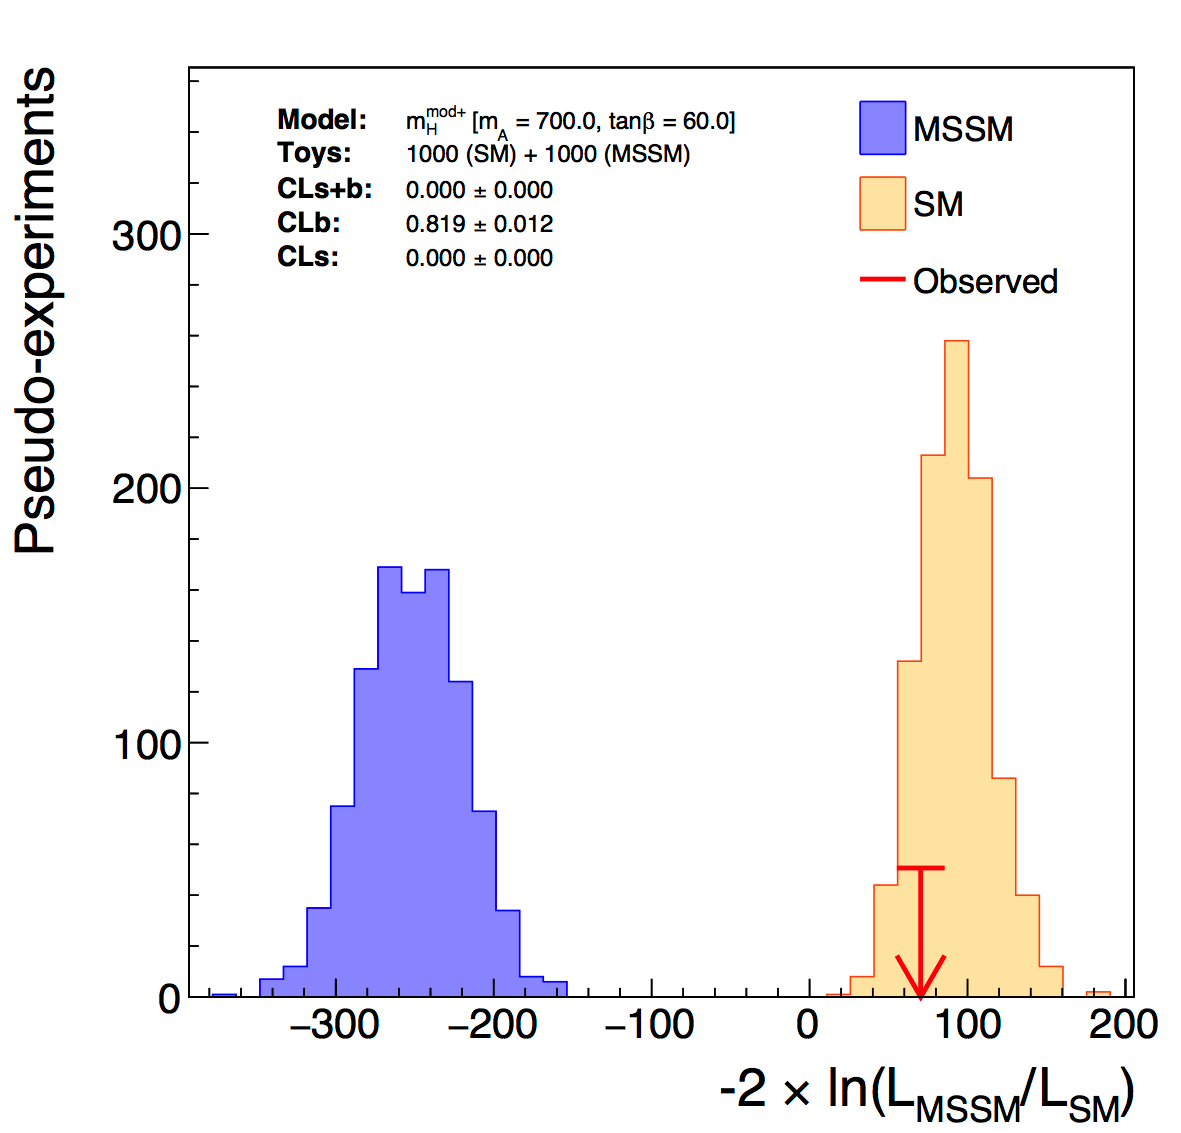
\includegraphics[width=0.5\textwidth]{./MSSM/Figures/plot_mA_700_tanb_60.png}}
\end{center}
\caption[Probability density functions for the SM and MSSM hypotheses at three different points in the $m_{\text{h}}^{\text{mod+}}$ scenario.]{Probability density functions, obtained by generating a large number of toy datasets, for the SM and MSSM hypotheses at three different points in the $m_{\text{h}}^{\text{mod+}}$
scenario, each with different levels of separation between the MSSM and SM distributions.}
\label{fig:mssm_mssmvssm_toys}
\end{figure}

\section{Results}
\label{sec:mssm_results}
\subsection{Model--independent results}
\label{sec:mssm_results_modelindep}
The \mTtot~distributions in the no b-tag and b-tag
categories of all channels, after the fit to the observed
data has been performed, are shown in figures \ref{fig:mssm_results_mttot_mt}--\ref{fig:mssm_results_mttot_em}.
The signal of the 3 neutral Higgs bosons at \mA=1 TeV and \tanb=50 in the $m_{h}^{mod+}$ scenario is overlaid 
on the total transverse mass distributions. The signal peaks twice due to the presence of a light Higgs boson
with mass compatible with 125 GeV in this model, which is necessary to incorporate the Higgs boson
observed at 125 GeV.

\begin{figure}[h!]
\begin{center}
\subfloat[no b-tag]{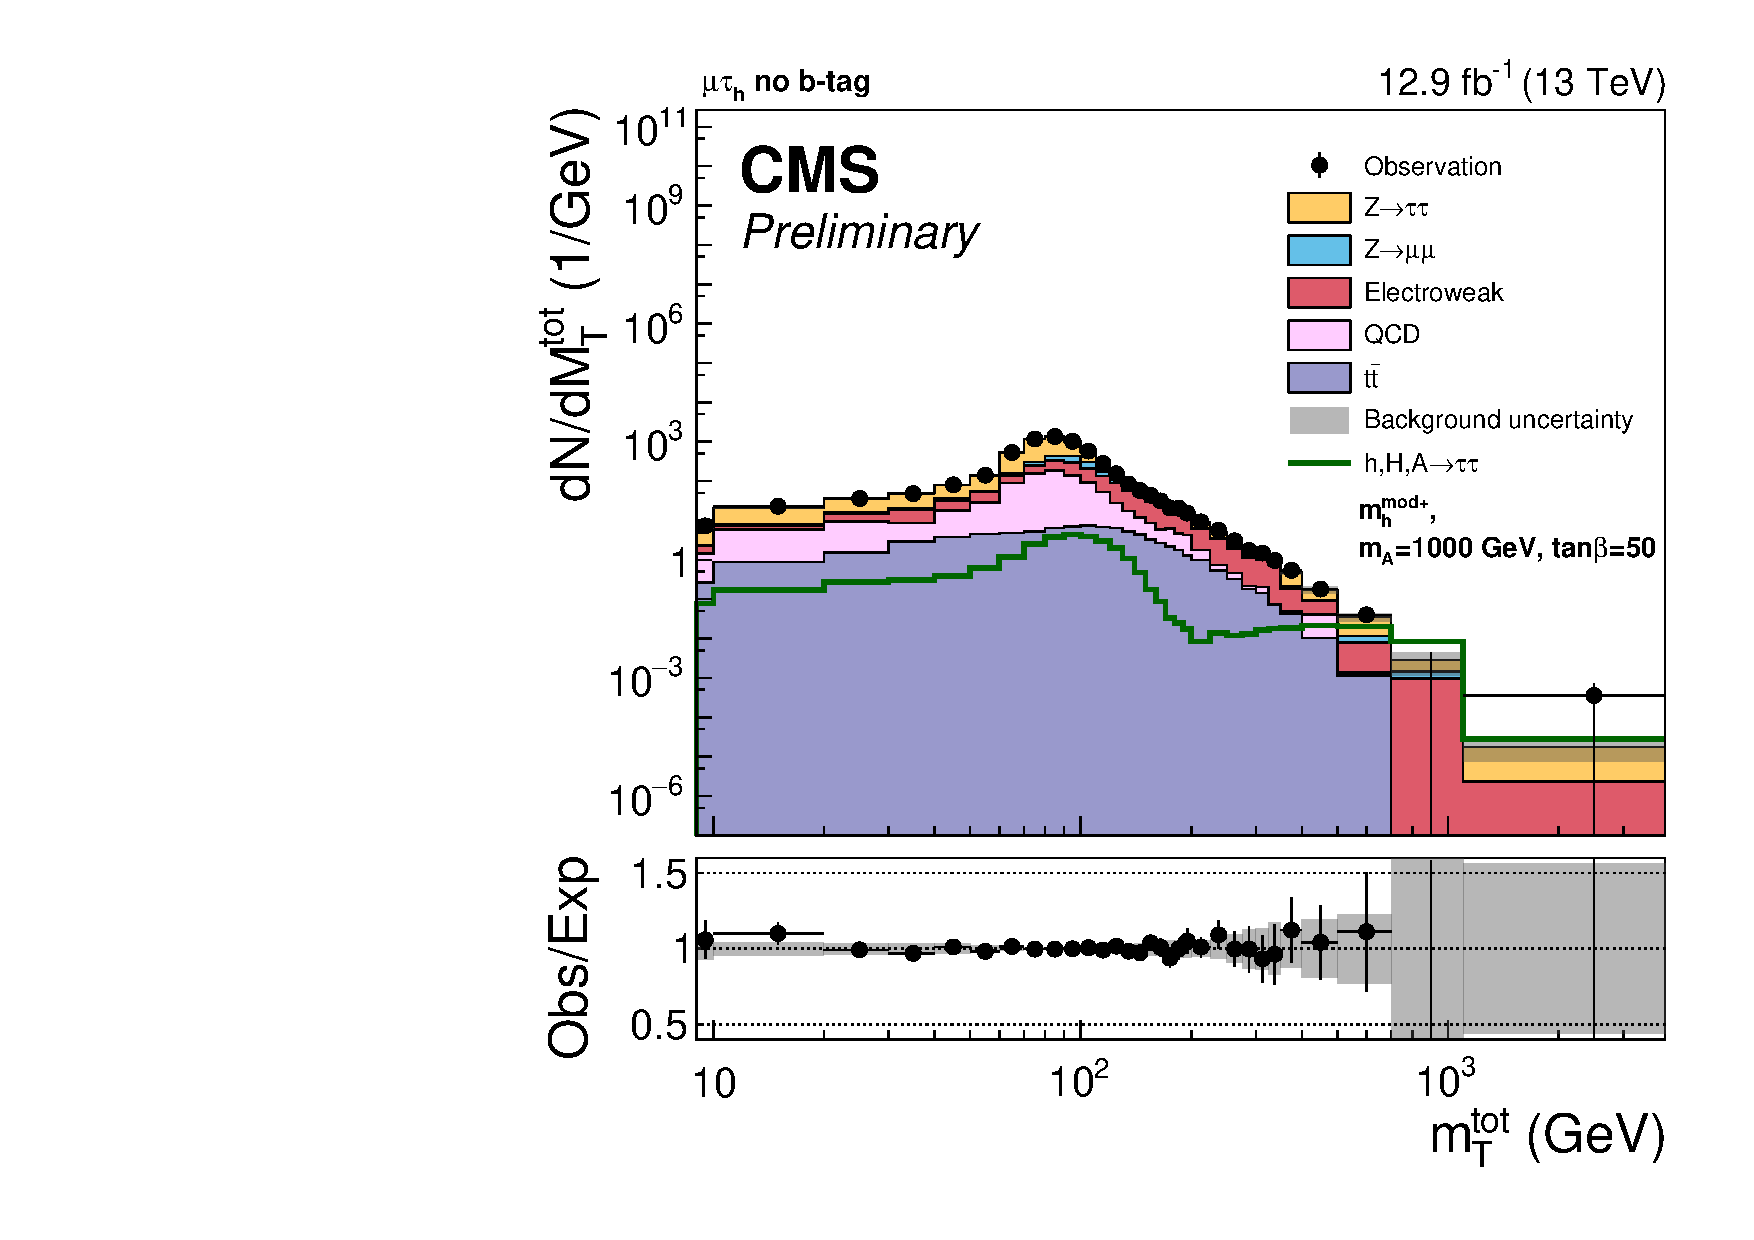
\includegraphics[width=0.5\textwidth]{MSSM/Figures/CMS-PAS-HIG-16-037_Figure_005-a.pdf}}
\subfloat[b-tag]{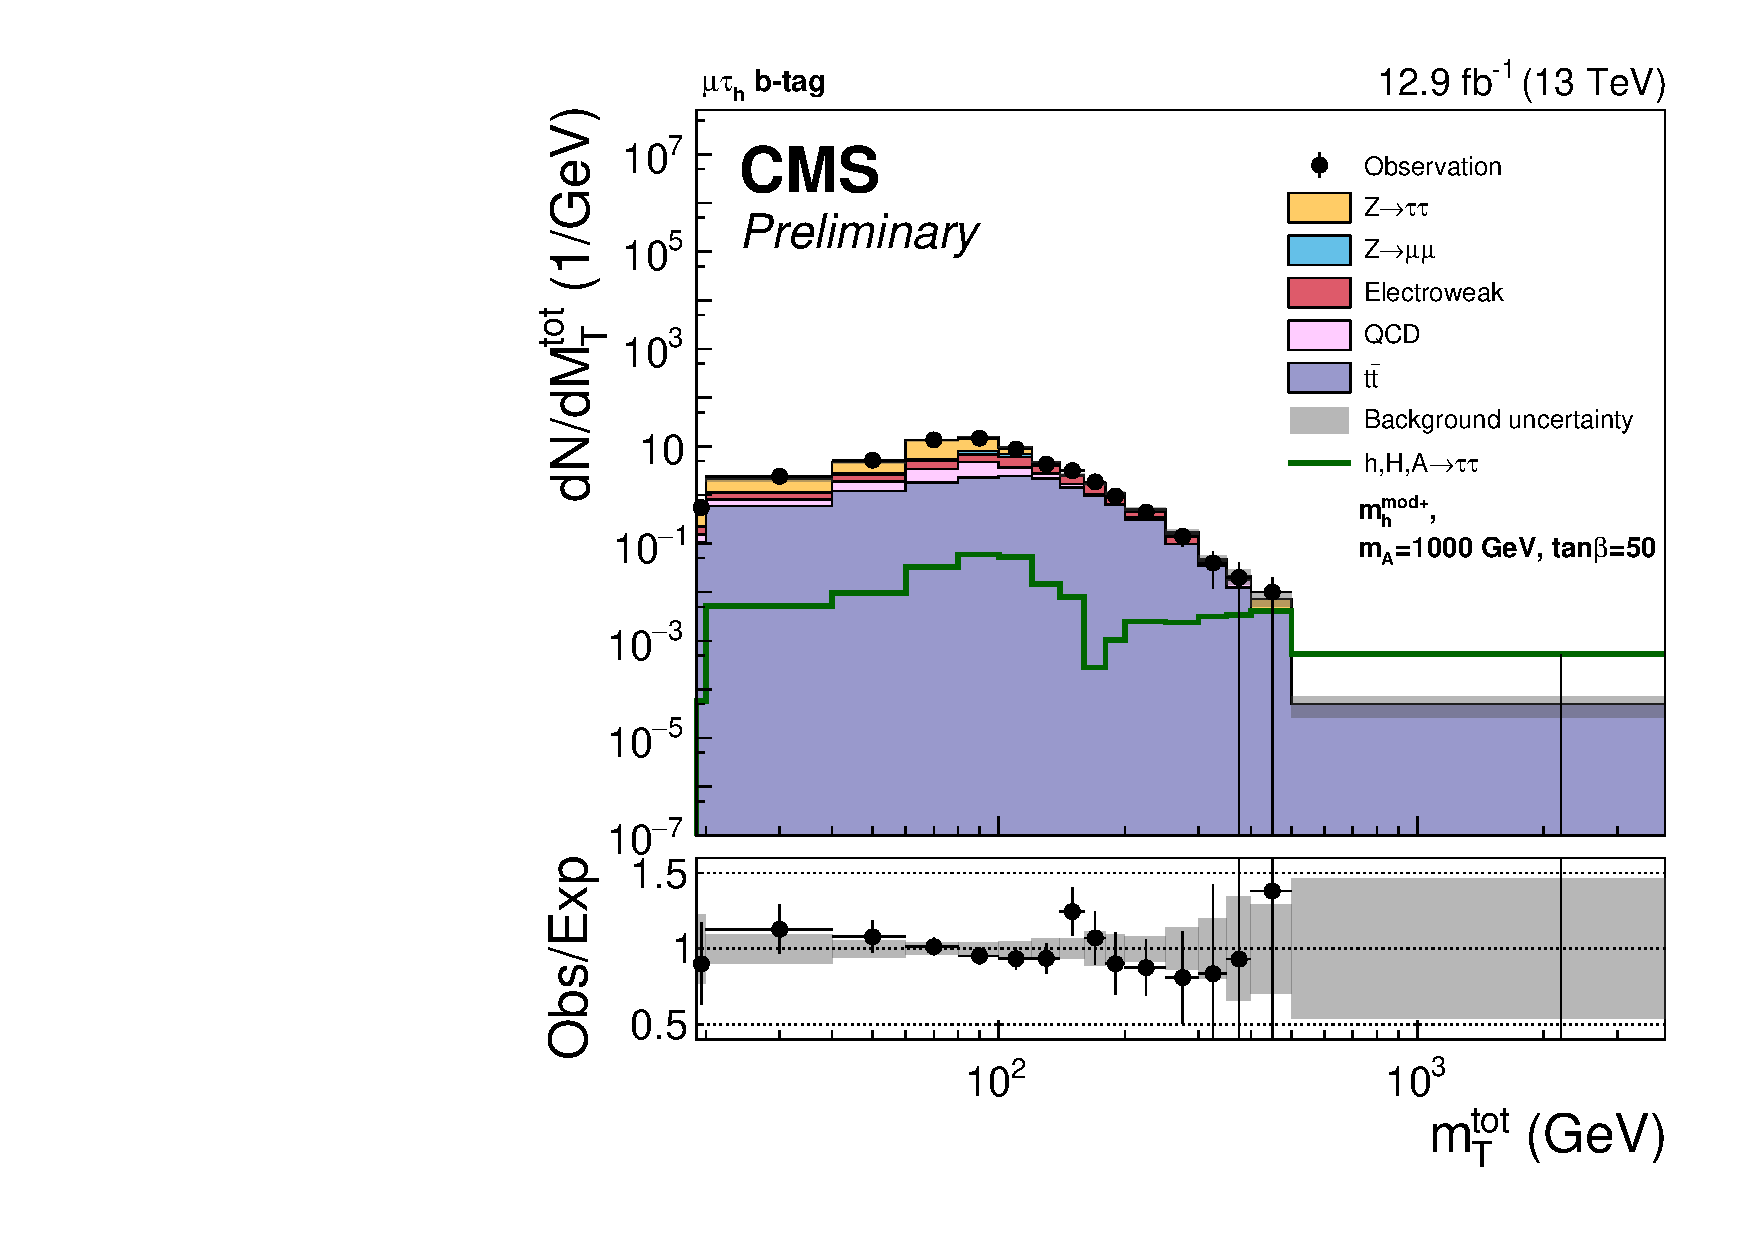
\includegraphics[width=0.5\textwidth]{MSSM/Figures/CMS-PAS-HIG-16-037_Figure_005-b.pdf}}
\end{center}
\caption[Distributions of \mTtot~in the no b-tag and b-tag categories
of the \mutau channel.]{Distributions of \mTtot~in the (a) no b-tag and (b) b-tag categories 
of the \mutau channel. The signal of the 3 neutral Higgs bosons at \mA=1 TeV 
and \tanb=50 in the $m_{h}^{mod+}$ scenario is overlaid. Note that, to incorporate
the observed Higgs boson at 125 GeV, the $m_{h}^{mod+}$ scenario includes a h boson
at around 125 GeV with a much larger $\sigma \times$BR than the 1 TeV H and A, and this is
the reason for the doubly--peaking shape of the overlaid signal \cite{CMS-PAS-HIG-16-037}.}
\label{fig:mssm_results_mttot_mt}
\end{figure}

\begin{figure}[h!]
\begin{center}
\subfloat[no b-tag]{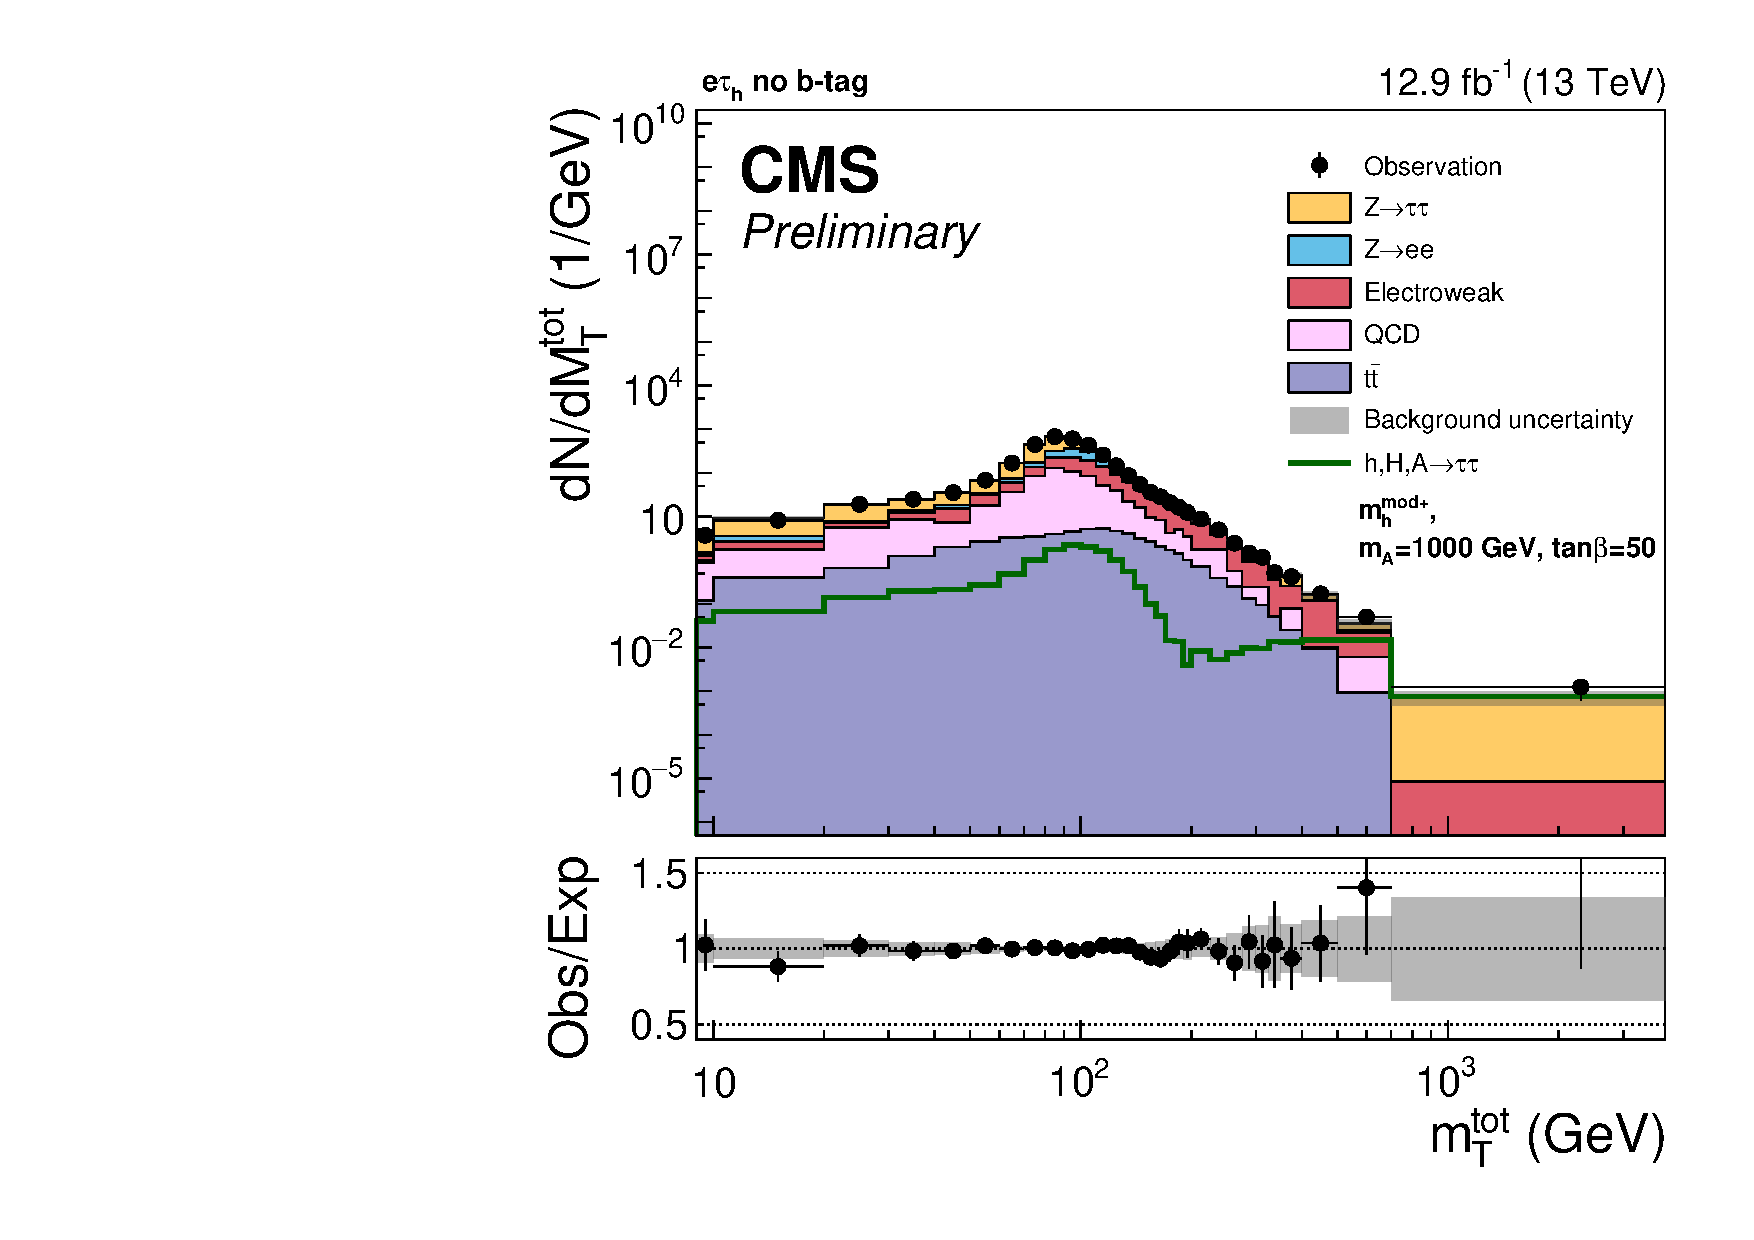
\includegraphics[width=0.5\textwidth]{MSSM/Figures/CMS-PAS-HIG-16-037_Figure_006-a.pdf}}
\subfloat[b-tag]{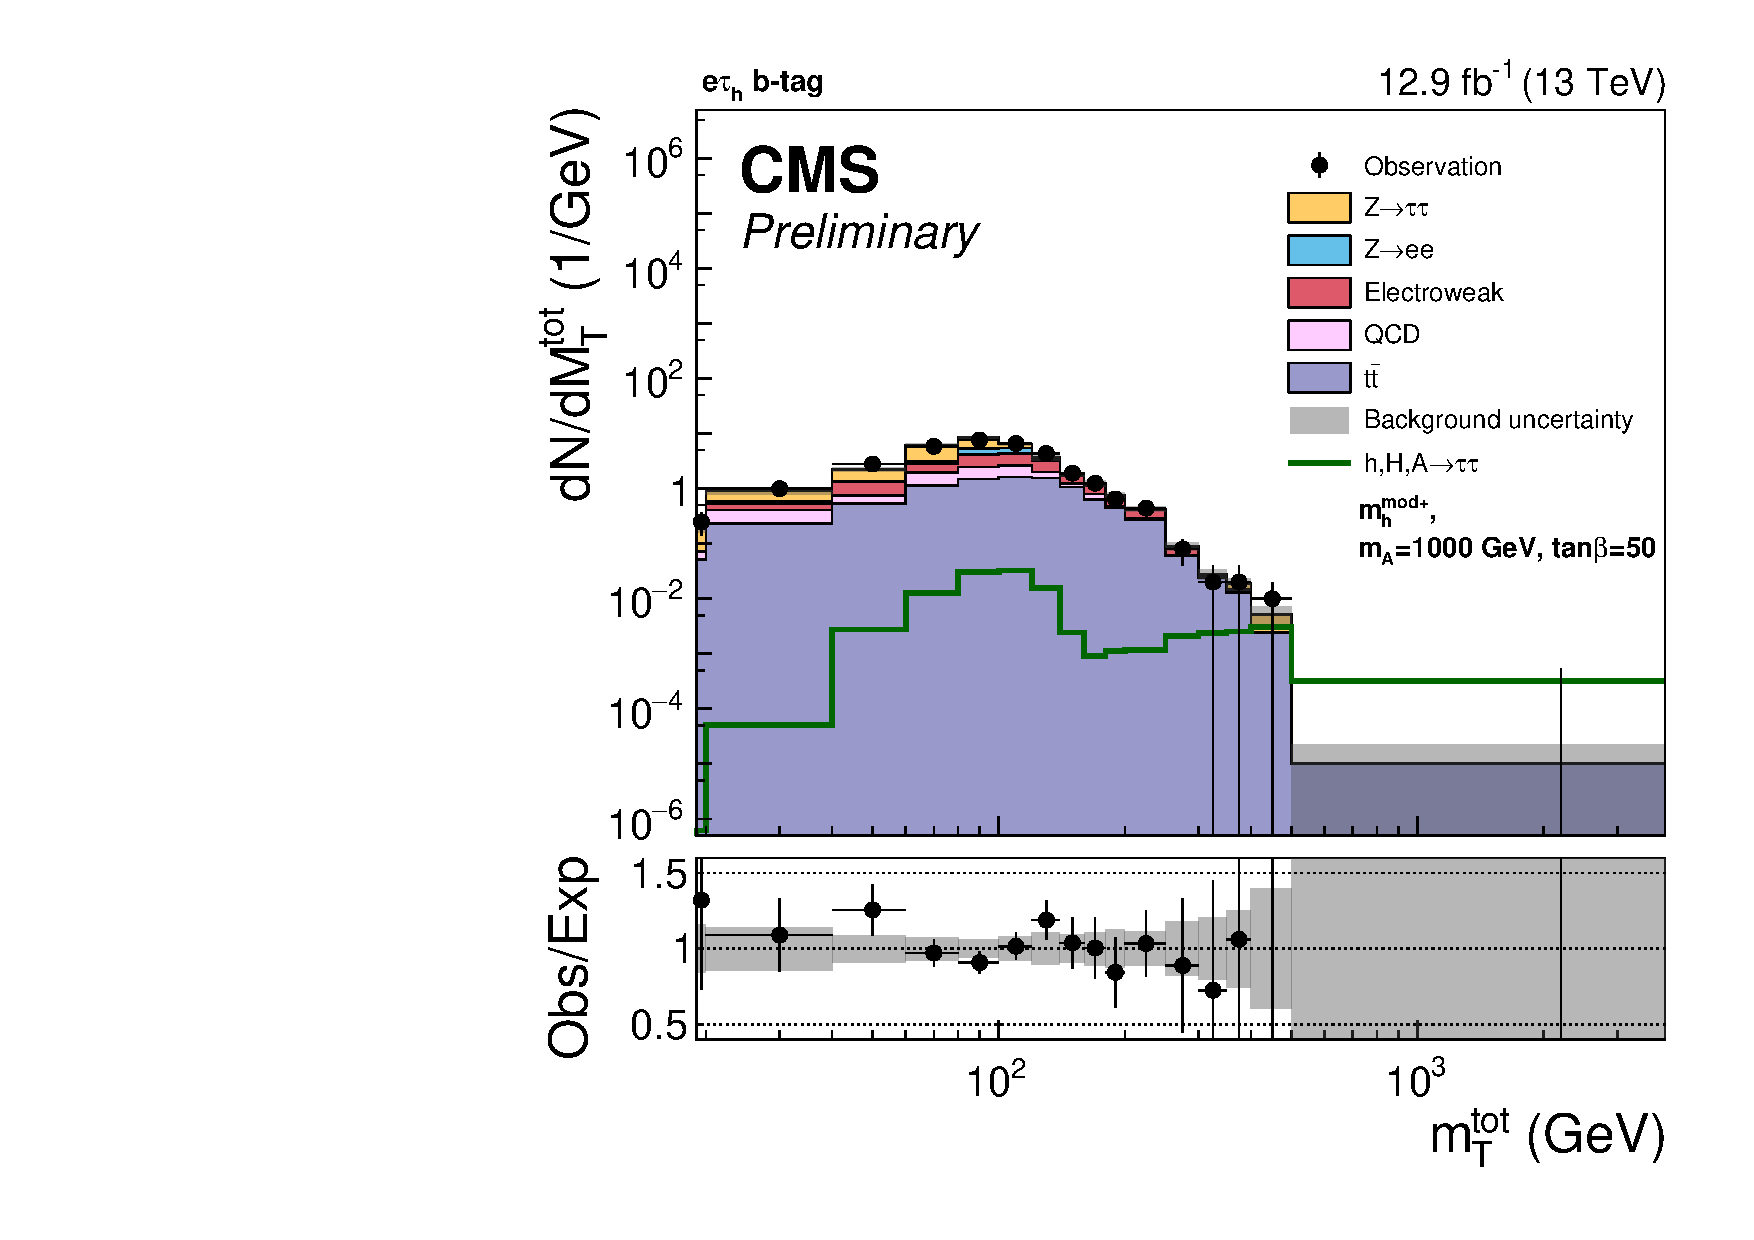
\includegraphics[width=0.5\textwidth]{MSSM/Figures/CMS-PAS-HIG-16-037_Figure_006-b.pdf}}
\end{center}
\caption[Distributions of \mTtot~inthe no b-tag and b-tag 
categories of the \etau channel.]{Distributions of \mTtot~in the (a) no b-tag and (b) b-tag categories 
of the \etau channel. The signal of the 3 neutral Higgs bosons at \mA=1 TeV 
and \tanb=50 in the $m_{h}^{mod+}$ scenario is overlaid \cite{CMS-PAS-HIG-16-037}.}% Note that, to incorporate
%the observed Higgs boson at 125 GeV, the $m_{h}^{mod+}$ scenario includes a h boson
%at around 125 GeV with a much larger $\sigma \times$BR than the 1 TeV H and A, and this is
%the reason for the doubly--peaking shape of the overlaid signal \cite{CMS-PAS-HIG-16-037}.}
\label{fig:mssm_results_mttot_et}
\end{figure}

\begin{figure}[h!]
\begin{center}
\subfloat[no b-tag]{\includegraphics[width=0.5\textwidth]{MSSM/Figures/CMS-PAS-HIG-16-037_Figure_008-a.pdf}}
\subfloat[b-tag]{\includegraphics[width=0.5\textwidth]{MSSM/Figures/CMS-PAS-HIG-16-037_Figure_008-b.pdf}}
\end{center}
\caption[Distributions of \mTtot~in the no b-tag and b-tag categories
of the \tautau channel.]{Distributions of \mTtot~in the (a) no b-tag and (b) b-tag categories 
of the \tautau channel. The signal of the 3 neutral Higgs bosons at \mA=1 TeV 
and \tanb=50 in the $m_{h}^{mod+}$ scenario is overlaid \cite{CMS-PAS-HIG-16-037}.}% Note that, to incorporate
%the observed Higgs boson at 125 GeV, the $m_{h}^{mod+}$ scenario includes a h boson
%at around 125 GeV with a much larger $\sigma \times$BR than the 1 TeV H and A, and this is
%the reason for the doubly--peaking shape of the overlaid signal \cite{CMS-PAS-HIG-16-037}.}
\label{fig:mssm_results_mttot_tt}
\end{figure}

\begin{figure}[h!]
\begin{center}
\subfloat[no b-tag]{\includegraphics[width=0.5\textwidth]{MSSM/Figures/CMS-PAS-HIG-16-037_Figure_007-a.pdf}}
\subfloat[b-tag]{\includegraphics[width=0.5\textwidth]{MSSM/Figures/CMS-PAS-HIG-16-037_Figure_007-b.pdf}}
\end{center}
\caption[Distributions of \mTtot~in the no b-tag and b-tag categories of 
the \emu channel.]{Distributions of \mTtot~in the (a) no b-tag and (b) b-tag categories 
of the \emu channel. The signal of the 3 neutral Higgs bosons at \mA=1 TeV 
and \tanb=50 in the $m_{h}^{mod+}$ scenario is overlaid \cite{CMS-PAS-HIG-16-037}.}% Note that, to incorporate
%the observed Higgs boson at 125 GeV, the $m_{h}^{mod+}$ scenario includes a h boson
%at around 125 GeV with a much larger $\sigma \times$BR than the 1 TeV H and A, and this is
%the reason for the doubly--peaking shape of the overlaid signal \cite{CMS-PAS-HIG-16-037}.}
\label{fig:mssm_results_mttot_em}
\end{figure}

None of these distributions show a significant excess. The
95\% CL upper limits on $\sigma\times$BR are shown in figure \ref{fig:mssm_results_limits}a
for gluon fusion and in figure \ref{fig:mssm_results_limits}b for b--associated
production. All channels and categories are combined. 
\begin{figure}[h!]
\begin{center}
\subfloat[gg$\phi$]{\includegraphics[width=0.5\textwidth]{MSSM/Figures/CMS-PAS-HIG-16-037_Figure_009-a.pdf}}
\subfloat[bb$\phi$]{\includegraphics[width=0.5\textwidth]{MSSM/Figures/CMS-PAS-HIG-16-037_Figure_009-b.pdf}}
\end{center}
\caption[Upper limits at 95\% CL for the gluon fusion production process and the
b-associated production process, combining all final states and categories.]{Upper limits at 95\% CL for (a) the gluon fusion production
process and (b) the b--associated production process. All four final states and 
all categories are combined for these limits. The green and yellow bands indicate
the $\pm 1\sigma$(68\%) and $\pm 2\sigma$(95\%) probability intervals on the expected limit \cite{CMS-PAS-HIG-16-037}.}
\label{fig:mssm_results_limits}
\end{figure}

A comparison of the expected limits
per channel is shown in figure \ref{fig:mssm_results_limits_breakdown}a for gg$\phi$ production
and in figure \ref{fig:mssm_results_limits_breakdown}b for bb$\phi$ production.
These figures show that the \mutau channel is the most sensitive at masses up to 
200 GeV, beyond which the \tautau channel becomes more sensitive. The \etau
channel is always slightly less sensitivie than the \mutau channel. The \emu channel
is the least sensitive over a large part of the parameter space, until it overtakes the 
\etau channel in sensitivity at 1.6 TeV and is slightly more sensitive than the
\mutau channel at 3.2 TeV. The \emu channel becomes more sensitive at higher masses as
a narrower binning of the \mTtot~distribution is possible than for the other channels.
The \mTtot~distribution for the high mass signals is therefore wide enough not to
fall entirely into the last bin used for the fit. This means at high mass this channel
benefits more from the shape discrimination between signal and backgrounds than
the other channels.

\begin{figure}[h!]
\begin{center}
\subfloat[gg$\phi$]{\includegraphics[width=0.5\textwidth]{MSSM/Figures/mssm_hig16037_limitcomp_ggh.pdf}}
\subfloat[bb$\phi$]{\includegraphics[width=0.5\textwidth]{MSSM/Figures/mssm_hig16037_limitcomp_bbh.pdf}}
\end{center}
\caption[Comparison of expected upper limits at 95\% CL for gluon fusion and 
b-associated production per channel.]{Expected upper limits at 95\% CL for (a) gluon fusion and (b) b--associated production,
comparing the combination of all channels (green) with the \mutau (red), \etau (blue) \tautau (black)
and \emu (gold) channels. For masses below 200 GeV the \mutau channel is the most sensitive,
while the \tautau channel dominates for higher masses. The \etau channel is always
slightly less sensitive than the \mutau channel. The \emu channel is the least sensitive, 
until at around 1.6 TeV it starts to overtake the \etau channel, with the sensitivity at 3.2 TeV 
being similar or slightly better than the \mutau channel.}
\label{fig:mssm_results_limits_breakdown}
\end{figure}

\clearpage

\subsection{Sensitivity to the standard model Higgs boson}
\label{sec:mssm_results_125GeV}
As we set limits on MSSM Higgs boson production 
down to masses of 90 GeV it is important to consider possible sensitivity
to the 125 GeV SM Higgs boson. As the cross--section times branching ratio for gluon fusion
production of the 125 GeV Higgs boson in the standard model, with decay into $\Pgt\Pgt$,
is 3.05 pb \cite{YR4} and the expected limit on cross--section times
branching ratio for MSSM gg$\phi$ production at around 125 GeV is around 20 pb
the analysis is not yet sensitive to the SM Higgs boson. The
limits shown in figure \ref{fig:mssm_results_greenband},
which include the standard model Higgs boson as part of the backgrounds,
are almost exactly the same as those shown in figure \ref{fig:mssm_results_limits}, which
also indicates the current lack of sensitivity to the standard model Higgs boson.

\begin{figure}[h!]
\begin{center}
\subfloat[gg$\phi$]{\includegraphics[width=0.5\textwidth]{MSSM/Figures/CMS-PAS-HIG-16-037_Figure-aux_005-a.pdf}}
\subfloat[bb$\phi$]{\includegraphics[width=0.5\textwidth]{MSSM/Figures/CMS-PAS-HIG-16-037_Figure-aux_005-b.pdf}}
\end{center}
\caption[Upper limits at 95\% CL for the gluon fusion and b-associated production processes, with the 125 GeV Higgs boson included as one of the backgrounds.]{Upper limits at 95\% CL for (a) the gluon fusion production
process and (b) the b--associated production process. The SM, 125 GeV Higgs boson
is included as one of the backgrounds. All four final states and 
all categories are combined for these limits. The light and dark green bands indicate
the $\pm 1\sigma$(68\%) and $\pm 2\sigma$(95\%) probability intervals on the expected limit \cite{CMS-PAS-HIG-16-037-addit}.}
\label{fig:mssm_results_greenband}
\end{figure}


\subsection{2D likelihood scans}
\label{sec:mssm_results_2D}
The 2D likelihood scans, as described in section \ref{sec:mssm_sigext_profile},
are shown in figure \ref{fig:mssm_results_2D_scans}
for four mass points ranging from 100 GeV to 3.2 TeV. The black cross indicates the best-fit value, with the red diamond showing the expected
best-fit value in the presence of the 125 GeV SM Higgs boson. The dark and light purple contours
indicate the 68\% and 95\% confidence interval, respectively.  From the shape of the contours
we can see the correlation between the gg$\phi$ and bb$\phi$ processes, illustrating
the fact that we cannot fully disentangle the two processes.

\begin{figure}[h!]
\begin{center}
\subfloat[$m_{\phi} = 100$ GeV]{\includegraphics[width=0.5\textwidth]{./MSSM/Figures/CMS-PAS-HIG-16-037_Figure_011-a.pdf}}
\subfloat[$m_{\phi} = 700$ GeV]{\includegraphics[width=0.5\textwidth]{./MSSM/Figures/CMS-PAS-HIG-16-037_Figure_011-g.pdf}}~\\
\subfloat[$m_{\phi} = 1.6$ TeV]{\includegraphics[width=0.5\textwidth]{./MSSM/Figures/CMS-PAS-HIG-16-037_Figure_011-i.pdf}}
\subfloat[$m_{\phi} = 3.2$ TeV]{\includegraphics[width=0.5\textwidth]{./MSSM/Figures/CMS-PAS-HIG-16-037_Figure_011-l.pdf}}
\end{center}
\caption[2D likelihood scans showing the best-fit value for cross--section 
times branching ratio of both the gluon fusion and b-associated production 
processes.]{2D likelihood scans showing the best-fit value (black cross) for cross--section times branching ratio 
of both the gluon fusion (x-axis) and b- associated production (y-axis) processes. The red diamond indicates the
expected best fit point for the presence of a 125 GeV SM Higgs boson, and the purple bands indicate the 68\% and
95\% confidence interval contours \cite{CMS-PAS-HIG-16-037}.}
\label{fig:mssm_results_2D_scans}
\end{figure}

\subsection{Interpretation in MSSM benchmark scenarios}
\label{sec:mssm_results_modeldep}
The results are interpreted in two MSSM benchmark scenarios: the $m_{\text{h}}^{\text{mod+}}$
scenario and the hMSSM scenario. Both scenarios are described in chapter \ref{chap:theory}.

Figure \ref{fig:mssm_mhmodp_2016}a shows the expected (dashed line and grey bands) and
observed (blue shaded area bounded by solid line) exclusion of the search presented in this chapter
in the \mA-\tanb~ plane of the $m_{\text{h}}^{\text{mod+}}$ scenario. The red shaded band
indicates the area that is excluded due to the lack of a light Higgs boson with a mass compatible
with 125 GeV. Compared with the most sensitive limits set during Run 1 of the \ac{LHC} these
limits at high \tanb~have been significantly improved, by around 300 GeV.

\begin{figure}[h!]
\begin{center}
\subfloat[$m_{h}^{\text{mod}+}$ scenario]{\includegraphics[width=0.65\textwidth]{./MSSM/Figures/CMS-PAS-HIG-16-037_Figure_012-a.pdf}}~\\
\subfloat[hMSSM scenario]{\includegraphics[width=0.65\textwidth]{./MSSM/Figures/CMS-PAS-HIG-16-037_Figure_012-b.pdf}}
\end{center}
\caption[Exclusion in the $m_{h}^{\text{mod+}}$ scenario and the hMSSM
scenario of the \AHtotautau analysis.]{Exclusion in (a) the $m_{h}^{\text{mod}+}$ scenario and (b) the hMSSM scenario 
obtained by the combination
of all channels in the \AHtotautau analysis. The blue shaded area bounded by the 
solid black line is the observed exclusion, with the dashed black line the
expected exclusion. The light and dark grey bands indicate
the $\pm 1\sigma$(68\%) and $\pm 2\sigma$(95\%) probability intervals on the expected limit.
The red shaded area in the $m_{h}^{\text{mod}+}$ figure
is excluded by the lack of a light Higgs boson with mass compatible with 125 GeV \cite{CMS-PAS-HIG-16-037}.}
\label{fig:mssm_mhmodp_2016}
\end{figure}

Figure \ref{fig:mssm_mhmodp_2016}b shows the expected (dashed line and grey bands)
and observed (blue shaded area bounded by solid line) exclusion of the search
presented in this chapter in the \mA-\tanb~plane of the hMSSM scenario. 
We should note again that this model, although defined for \tanb~ values
upwards of 10, is only strictly valid for \tanb~below 10.
The small excluded area around \mA=200 GeV is genuine. It is caused by the 
production cross-section times branching ratio in the model, which is driven by
two effects \cite{CMS-PAS-HIG-16-007}. On the one hand the branching ratio into taus decreases with decreasing
\tanb, while on the other hand a negative top--bottom interference effect increases the
gluon fusion cross--section with decreasing \tanb. Therefore the
combined cross--section times branching ratio decreases with decreasing \tanb, until it
increases again from a low value of \tanb~down to \tanb=1. The feature is 
thus expected to grow with more data.

\chapter{Combination of MSSM analyses}
\label{sec:mssm_combination}
The results of the search for neutral Higgs bosons in the MSSM using the di-tau
final state, using a dataset
corresponding to an integrated luminosity of 12.9 fb$^{-1}$, collected during the
first half of 2016 and thus referred to as `2016 analysis', can be combined 
with a previous search. This previous analysis
was performed on a dataset corresponding to an integrated luminosity of 2.3 fb$^{-1}$
collected during 2015 (`2015 analysis'), and is detailed in Ref. \cite{CMS-PAS-HIG-16-006}.
By combining the two analyses we should be able to set the most stringent
limits on the two MSSM production modes, and in the \mA-\tanb~plane of 
MSSM benchmark scenarios, available at the time of writing. It is also
a first step on the way to combining the \AHtotautau analysis with
searches for charged Higgs bosons or heavy neutral Higgs bosons in 
other final states. 

The 2015 analysis uses the same channels, categories, and very
similar background estimation methods as the 2016 analysis and so
it is not described in detail. The results of the analysis will 
be presented, and key differences with the more recent result highlighted
where needed.

\section{Results from the 2015 analysis}
\label{sec:mssm_combination_2015}
As for the analysis presented in 
chapter \ref{chap:mssm} a shape analysis is performed, however a different
discriminating variable is used. The variable used is the transverse component of the di-$\Pgt$ mass
as reconstructed using the \texttt{SVFit} algorithm, 
denoted $m_{\text{T},\tau\tau}$. The transverse di-$\Pgt$ mass 
distributions for the signal region categories of the four channels are shown in figures \ref{fig:mssm_hig16006_mtsv_mt} -- \ref{fig:mssm_hig16006_mtsv_em}.
\begin{figure}[h!]
\begin{center}
\subfloat[No b-tag]{\includegraphics[width=0.5\textwidth]{./MSSM/Figures/htt_mt_8_hig16006_shapeshig16006_postfit_logy_logx.pdf}}
\subfloat[B-tag]{\includegraphics[width=0.5\textwidth]{./MSSM/Figures/htt_mt_9_hig16006_shapeshig16006_postfit_logy_logx.pdf}}
\end{center}
\caption[Transverse component of the di-\Pgt mass for expected backgrounds
and observed events in the no b-tag and b-tag categories of the \mutau channel.]{Transverse component of the di-$\Pgt$ mass for expected backgrounds and
observed events in the (a) no b-tag and (b) b-tag categories of the \mutau channel.
The signal overlaid corresponds to the signal of the three Higgs bosons at \mA=1 TeV and \tanb=50
in the $m_{\text{h}}^{\text{mod+}}$ scenario, and so it peaks once at low mass, for the light Higgs boson,
and once at higher mass, for the heavy H and A.}
\label{fig:mssm_hig16006_mtsv_mt}
\end{figure}

\begin{figure}[h!]
\begin{center}
\subfloat[No b-tag]{\includegraphics[width=0.5\textwidth]{./MSSM/Figures/htt_et_8_hig16006_shapeshig16006_postfit_logy_logx.pdf}}
\subfloat[B-tag]{\includegraphics[width=0.5\textwidth]{./MSSM/Figures/htt_et_9_hig16006_shapeshig16006_postfit_logy_logx.pdf}}
\end{center}
\caption[Transverse component of the di-\Pgt mass for expected backgrounds
and observed events in the no b-tag and b-tag categories of the \etau channel.]{Transverse component of the di-$\Pgt$ mass for expected backgrounds and
observed events in the (a) no b-tag and (b) b-tag categories of the \etau channel.}
%The signal overlaid corresponds to the signal of the three Higgs bosons at \mA=1 TeV and \tanb=50
%in the $m_{\text{h}}^{\text{mod+}}$ scenario, and so it peaks once at low mass, for the light Higgs boson,
%and once at higher mass, for the heavy H and A.}
\label{fig:mssm_hig16006_mtsv_et}
\end{figure}

\begin{figure}[h!]
\begin{center}
\subfloat[No b-tag]{\includegraphics[width=0.5\textwidth]{./MSSM/Figures/htt_tt_8_hig16006_shapeshig16006_postfit_logy_logx.pdf}}
\subfloat[B-tag]{\includegraphics[width=0.5\textwidth]{./MSSM/Figures/htt_tt_9_hig16006_shapeshig16006_postfit_logy_logx.pdf}}
\end{center}
\caption[Transverse component of the di-\Pgt mass for expected backgrounds
and observed events in the no b-tag and b-tag categories of the \tautau
channel.]{Transverse component of the di-$\Pgt$ mass for expected backgrounds and
observed events in the (a) no b-tag and (b) b-tag categories of the \tautau channel.}
%The signal overlaid corresponds to the signal of the three Higgs bosons at \mA=1 TeV and \tanb=50
%in the $m_{\text{h}}^{\text{mod+}}$ scenario, and so it peaks once at low mass, for the light Higgs boson,
%and once at higher mass, for the heavy H and A.}
\label{fig:mssm_hig16006_mtsv_tt}
\end{figure}

\begin{figure}[h!]
\begin{center}
\subfloat[No b-tag]{\includegraphics[width=0.5\textwidth]{./MSSM/Figures/htt_em_8_hig16006_shapeshig16006_postfit_logy_logx.pdf}}
\subfloat[B-tag]{\includegraphics[width=0.5\textwidth]{./MSSM/Figures/htt_em_9_hig16006_shapeshig16006_postfit_logy_logx.pdf}}
\end{center}
\caption[Transverse component of the di-\Pgt mass for expected backgrounds
and observed events in the no b-tag and b-tag cateogires of the \emu channel.]{Transverse component of the di-$\Pgt$ mass for expected backgrounds and
observed events in the (a) no b-tag and (b) b-tag categories of the \emu channel.}
%The signal overlaid corresponds to the signal of the three Higgs bosons at \mA=1 TeV and \tanb=50
%in the $m_{\text{h}}^{\text{mod+}}$ scenario, and so it peaks once at low mass, for the light Higgs boson,
%and once at higher mass, for the heavy H and A.}
\label{fig:mssm_hig16006_mtsv_em}
\end{figure}

These distributions do not show any significant excesses. The upper limits
on cross--section times branching ratio for the gluon fusion and b-associated production
processes are shown in figure \ref{fig:mssm_results_hig16006_limits}a
and b, respectively. All channels and categories are combined. A comparison of
the expected limits per channel is given in figure \ref{fig:mssm_results_limits_breakdown_hig16006}.
These follow a similar pattern to those given in figure \ref{fig:mssm_results_limits_breakdown}, notice
however the \emu channel remains the least sensitive even at very high mass, as the
transverse component of the di-$\Pgt$ mass exhibits a sizeable \ttbar tail in the \emu channel. The total
transverse mass collapses events from the tail into lower regions of the distribution, thus reducing the backgrounds
at higher mass.

\begin{figure}[h!]
\begin{center}
\subfloat[gg$\phi$]{\includegraphics[width=0.5\textwidth]{MSSM/Figures/Figure_006-a.pdf}}
\subfloat[bb$\phi$]{\includegraphics[width=0.5\textwidth]{MSSM/Figures/Figure_006-b.pdf}}
\end{center}
\caption[Upper limits at 95\% CL for the gluon fusion and b-associated production process.]{Upper limits at 95\% CL for (a) the gluon fusion production
process and (b) the b--associated production process. All four final states and 
all categories are combined for these limits. The green and yellow bands indicate
the $\pm 1\sigma$(68\%) and $\pm 2\sigma$(95\%) probability intervals on the expected limit  \cite{CMS-PAS-HIG-16-006}.}
\label{fig:mssm_results_hig16006_limits}
\end{figure}

\begin{figure}[h!]
\begin{center}
\subfloat[gg$\phi$]{\includegraphics[width=0.5\textwidth]{MSSM/Figures/mssm_hig16006_limitcomp_ggH.pdf}}
\subfloat[bb$\phi$]{\includegraphics[width=0.5\textwidth]{MSSM/Figures/mssm_hig16006_limitcomp_bbH.pdf}}
\end{center}
\caption[Expected upper limits at 95\% CL for the gluon fusion and b-associated
production, comparing the combination of all channels with the per-channel limits.]{Expected upper limits at 95\% CL for (a) gluon fusion and (b) b--associated production,
comparing the combination of all channels (green) with the \mutau (red), \etau (blue) \tautau (black)
and \emu (gold) channels. For masses below 200 GeV the \mutau channel is the most sensitive,
while the \tautau channel dominates for higher masses. The \etau channel is always
slightly less sensitive than the \mutau channel. The \emu channel is the least sensitive.}
\label{fig:mssm_results_limits_breakdown_hig16006}
\end{figure}
\clearpage


\section{Combination procedure}
\label{sec:mssm_combination_procedure}
The idea of combining the two analyses is to combine the 
individual likelihoods to improve the analysis sensitivity and
physics reach. To do this correctly the correlations between
nuisance parameters in the 2015 and 2016 analyses need to be taken into account.

The choice of correlation scheme is decided on
based on the procedure used for the ATLAS and \ac{CMS}
Higgs combinations \cite{MassComb,CouplComb}. This means
uncertainties are either considered 100\% correlated or fully uncorrelated. Partial
correlations are not taken into account, with a small number of exceptions. The
correlations used for this combination are given in table \ref{tab:mssm_combination_correlations},
with the motivation for the chosen correlation given in the third column of the table.
The chosen correlation scheme is motivated
by carefully considering the differences between the two analyses
and the conditions under which they were performed.

%The correct way to establish the correlations is to perform
%dedicated studies into them. In many cases such studies would be 
%unfeasible to perform, or it would not be clear how to approach the 
%problem in the first place.
%Even without performing these studies, a choice of correlation scheme can be motivated
%by carefully considering the differences between the two analyses and the conditions
%under which they were performed.
%This is what has been done for this combination.
%Strictly, studies into the underlying correlations between
%nuisance parameters should be performed. This is however not always
%feasible and in some cases
%The correlation scheme between nuisance parameters relating to the 2015 and 2016
%analyses, as used for this combination, is given in table \ref{tab:mssm_combination_correlations}. 
%The third column of this table gives the motivation for the chosen correlation.

\begin{table}[htp]
\begin{center}
\caption{Correlations between nuisance parameters in the 2015 and 2016 analysis}
{\footnotesize
\begin{tabular}{p{3cm}p{2cm}p{10cm}}
\toprule
\textbf{Nuisance} & \textbf{Correlation} & \textbf{Motivation}\\
\midrule
Luminosity & Partially \mbox{correlated} & Recommended by the CMS collaborators who perform the luminosity measurement, after dedicated studies.\\
\midrule
Jet energy scale & Fully \mbox{correlated} & Recommended by the CMS collaborators who derive jet energy corrections, after dedicated studies.\\
\midrule
B-tagging & Uncorrelated & Scale factors used in the 2015 and 2016 analysis measured via different methods.\\
\midrule
Mis-tagging & Partially \mbox{correlated} & Recommended by the CMS collaborators responsible for deriving b-tagging scale factors, after dedicated studies.\\
\midrule
Muon ID/isolation/trigger & Uncorrelated & The 2015 and 2016 analyses use different muon ID and isolation working points, and the \ac{L1} trigger was replaced completely between 2015 and 2016.\\
\midrule
Electron ID/isolation/trigger & Uncorrelated & The \ac{L1} trigger was completely replaced between 2015 and 2016.\\
\midrule
Tau ID/isolation/trigger& Uncorrelated & \scriptsize{On top of the replacement of the \ac{L1} trigger, a tau ID scale factor was applied in the 2016 analysis but not in the 2015 analysis, despite an observed downward correction of 8\% on the yield of backgrounds with real hadronic taus.}\\
\midrule
High-\pT~tau ID \mbox{efficiency} & Correlated & This should not be affected by the lack of tau ID scale factor and covers the same underlying issue in both analyses.\\
\midrule
Tau energy scale & Correlated & There is no reason to expect a different best-fit energy scale between 2015 and 2016.\\
\midrule
Electron energy scale & Correlated & There is no reason to expect a different best-fit energy scale between 2015 and 2016.\\
\midrule
Drell-Yan shape & Correlated & \scriptsize{The same \ac{MC} samples, are used in 2014 and 2016 to derive the correction. The weights derived for the 2015 analysis and the 2016 analysis are very similar.}\\
\midrule
W jet$\rightarrow\Pgt_{h}$ fake rate shape & Uncorrelated & \scriptsize{Correction not applied in the 2016 dataset while it was applied for the 2015 analysis. The uncertainties have a different functional form, possibly due to different jet$\rightarrow\Pgt_{h}$ fake rates as a result of the use of a different tau isolation working point.}\\
\midrule
MET uncertainties & Correlated & The same MVA \MET training was used both for 2015 and 2016.\\
\midrule
\mbox{Top quark} \pT~reweighting & Correlated & The same corrections were applied to the 2015 and 2016 analyses.\\
\midrule
Drell-Yan $\sigma$& Correlated & The same recommended cross sections were used in 2015 and 2016.\\
\midrule
Di--boson $\sigma$ & Correlated & The same recommended cross sections were used in 2015 and 2016.\\
\midrule
\ttbar $\sigma$ & Correlated & The same recommended cross sections were used in 2015 and 2016.\\
\midrule
\Wjets $\sigma$ & Correlated & The same recommended cross section was used in 2015 and 2016..\\
\midrule
SM signal theory uncertainties & Correlated & The same recommende cross sections were used in 2015 and 2016..\\
\midrule
\Ztautau \mbox{acceptance} & N/A & \scriptsize{Uncertainty only exists in the 2015 analysis as no fits to the \Zmm control region were included.}\\
\midrule
\Ztautau \mbox{extrapolation}& N/A & \scriptsize{Uncertainty only exists in 2016 analysis as fits to the \Zmm control regions were included and this uncertainty should cover only the extrapolation from \Zmm to \Ztautau, not the full acceptance.}\\
\midrule
%e$\rightarrow\Pgt_{h}$ fake rate & Correlated & Expect to behave the same in 2015 and 2016 datasets.\\
%$\mu\rightarrow\Pgt_{h}$ fake rate & Uncorrelated & Measurement had not been made at time of 2015 analysis and so no scale factors were applied.\\
%jet$\rightarrow\Pgt_{h}$ fake rate & Correlated & ....\\
%QCD extrapolation uncertainty (\emu channel) & Uncorrelated & Use of slightly different anti-iso sideband in 2015 and 2016 analyses\\
%QCD normalisation uncertainty (\tautau channel) & Uncorrelated & Use of different anti-isolated sideband\\
%Parameters tying control regions to signal region normalisations & Uncorrelated & 2016 control region fits should not influence the 2015 signal region and vice versa\\
%Statistical uncertainty on W opposite--sign to same--sign ratio (\etau and \mutau)& Uncorrelated & Statistical uncertainties should not be correlated\\
%Systematic uncertainty on W opposite--sign to same--sign ratio (\etau and \mutau)& Uncorrelated & Uncertainty based on high \mT~ region with anti-isolated $\Pgt_{h}$, but because of the tau \pT~cuts being different in the 2015 and 2016 analyses we could expect a different event composition in this region. In addition this uncertainty was already uncorrelated between channels and categories in each individual analysis, and we can't claim to know the correlation between the two years any more accurately than that\\
%Statistical uncertainty on W low/high\mT~ ratio (\etau and \mutau)& Uncorrelated & Statistical uncertainties should not be correlated\\
%Systematic uncertainty on W low/high\mT~ ratio (\etau and \mutau) & Uncorrelated & This was already uncorrelated between channels and categories in each individual analysis, we can't claim to know the correlation between the two years any more accurately\\
%QCD OS/SS ratio statistical uncertainty (\etau and \mutau) & Uncorrelated & Statistical uncertainties should not be correlated\\
%QCD OS/SS ratio systematic uncertainty (\etau and \mutau) & Uncorrelated & The ratios were measured in different anti-isolated sidebands, and with different $\Pgt_{h}$ \pT~ selections, in the two analyses. Same comments about the correlations between channels and categories within the individual analyses as for the W systematic uncertainties apply.\\
%bin--by--bin uncertainties for templates with low numbers of events & Uncorrelated &Because the same initial \ac{MC} simulation was used these should in theory be correlated, in practice this is unfeasible to achieve\\
\end{tabular}}
\label{tab:mssm_combination_correlations}
\end{center}
\clearpage
\end{table}
\begin{table}[pt!]
\begin{center}
{\footnotesize
\begin{tabular}{p{3cm}p{2cm}p{10cm}}
\midrule
e$\rightarrow\Pgt_{h}$ fake rate & Correlated & Expected to behave the same in 2015 and 2016 datasets, the same anti-electron discriminator was used and the uncertainty on the fake rate should not be affected by the use of a different hadronic tau ID discriminator working point.\\
\midrule
$\mu\rightarrow\Pgt_{h}$ fake rate & Uncorrelated & Measurement had not been made at time of 2015 analysis and so no scale factors were applied yet, while this had changed for the 2016 analysis.\\
\midrule
jet$\rightarrow\Pgt_{h}$ fake rate & Correlated & Uncertainty on the jet$\rightarrow\Pgt_{h}$ fake rate should not be affected by changes in hadronic tau isolation working point.\\
\midrule
QCD extrapolation uncertainty (\emu channel) & Uncorrelated & Use of slightly different anti-isolated sideband in 2015 and 2016 analyses.\\
\midrule
QCD normalisation uncertainty (\tautau channel) & Uncorrelated & Use of different anti-isolated sideband.\\
\midrule
Parameters tying control regions to signal region normalisations & Uncorrelated & 2016 control region fits should not influence the 2015 SR and vice versa.\\
\midrule
Statistical \mbox{uncertainty} on W opposite--sign to same--sign ratio (\etau and \mutau)& Uncorrelated & Statistical uncertainties should not be correlated.\\
\midrule
Systematic \mbox{uncertainty} on W opposite--sign to same--sign ratio (\etau and \mutau)& Uncorrelated & \scriptsize{Uncertainty based on high \mT~ region with anti-isolated $\Pgt_{h}$, but because of the tau \pT~cuts being different in the 2015 and 2016 analyses we could expect a different event composition in this region. In addition this uncertainty was already uncorrelated between channels and categories in each individual analysis, and we can't claim to know the correlation between the two years any more accurately than that.}\\
\midrule
Statistical \mbox{uncertainty} on W low/high-\mT~\mbox{ratio} (\etau and \mutau)& Uncorrelated & Statistical uncertainties should not be correlated.\\
\midrule
Systematic \mbox{uncertainty} on W low/high-\mT~\mbox{ratio} (\etau and \mutau) & Uncorrelated & \scriptsize{This was already uncorrelated between channels and categories in each individual analysis, we can't claim to know the correlation between the two years any more accurately.}\\
\midrule
QCD OS/SS \mbox{ratio} statistical \mbox{uncertainty} (\etau and \mutau) & Uncorrelated & Statistical uncertainties should not be correlated.\\
\midrule
QCD OS/SS \mbox{ratio} systematic \mbox{uncertainty} (\etau and \mutau) & Uncorrelated & \scriptsize{The ratios were measured in different anti-isolated sidebands, and with different $\Pgt_{h}$ \pT~ selections, in the two analyses. Same comments about the correlations between channels and categories within the individual analyses as for the W systematic uncertainties apply.}\\
\midrule
bin--by--bin \mbox{uncertainties} for templates with low numbers of events & Uncorrelated &Because the same initial \ac{MC} simulation was used these should in theory be correlated, in practice this is unfeasible.\\
\bottomrule
\end{tabular}}
\end{center}
\end{table}
\clearpage



\section{Results}
\label{sec:mssm_combination_results}
The expected and observed upper limits on cross--section times branching ratio,
for the combination of the 2015 and 2016 analyses, are shown in figure
\ref{fig:mssm_results_combination_limits}. The limits behave as expected
from the individual 2015 and 2016 limits. 

\begin{figure}[h!]
\begin{center}
\subfloat[gg$\phi$]{\includegraphics[width=0.5\textwidth]{MSSM/Figures/mssm_combination_090117_ggH_cmb.png}}
\subfloat[bb$\phi$]{\includegraphics[width=0.5\textwidth]{MSSM/Figures/mssm_combination_090117_bbH_cmb.png}}
\end{center}
\caption[Upper limits at 95\% CL for the gluon fusion and b-associated production
process, obtained by combining all channels and categories of the 2015 nd the 2016 analyses.] {Upper limits at 95\% CL for (a) the gluon fusion production
process and (b) the b--associated production process. These results
combine all categories and all four final states from both the 2015
and the 2016 analyses. The green and yellow bands indicate
the $\pm 1\sigma$(68\%) and $\pm 2\sigma$(95\%) probability intervals on the expected limit.}
\label{fig:mssm_results_combination_limits}
\end{figure}

To get a better picture of how the sensitivity of the individual analyses compares
with the combination, we should consider the comparison
of expected limits in figure \ref{fig:mssm_results_combination_limits_comp}. The
gluon fusion limits in figure \ref{fig:mssm_results_combination_limits_comp}a show that at
higher masses the sensitivity is only very slightly improved with respect to the 
analysis of the 12.9 fb$^{-1}$ dataset. However, for masses between 200 and 800 GeV
there is a larger improvement in sensitivity from combining the two analyses.
This behaviour is expected since the 2016 analysis used a slightly different
selection that made the analysis more optimal at masses above 800 GeV,
and slightly less optimal below this mass. This
effect is less visible on the b--associated production limits shown in figure \ref{fig:mssm_results_combination_limits_comp}b.

\begin{figure}[h!]
\begin{center}
\subfloat[gg$\phi$]{\includegraphics[width=0.5\textwidth]{MSSM/Figures/mssm_combination_comparison_ggH_with_ratio.pdf}}
\subfloat[bb$\phi$]{\includegraphics[width=0.5\textwidth]{MSSM/Figures/mssm_combination_comparison_bbH_with_ratio.pdf}}
\end{center}
\caption[Comparison of the expected upper limits at 95\% CL for the 
gluon fusion and b-associated production process, comparing the 2015 and 2016 analyses with a combination.]{Comparison of the expected upper limits at 95\% CL for (a) the gluon fusion production
process and (b) the b--associated production process. The green curve shows the results
from combining the 2015 and 2016 analyses (integrated luminosity of 15.2 fb$^{-1}$),
with the red line indicating the limits from the 2016 analysis only (integrated luminosity of 12.9 fb$^{-1}$)
and the blue line indicating the limits from the 2015 analysis only (integrated luminosity of 2.3 fb$^{-1}$).
The plotted relative difference is with respect to the limits from the 2016 analysis, showing how the combination
improves on those limits by between a few per cent at high mass up to 40\% at low mass.}
\label{fig:mssm_results_combination_limits_comp}
\end{figure}

Interpretations in MSSM benchmark scenarios to be added.




